% !Mode:: "TeX:UTF-8"
% !TEX encoding = UTF-8 Unicode

%----------------------------------------------------------------------------------------
% Natural Language Processing: Neural Networks and Large Language Models
%
% Copyright 2021-2026
% Tong Xiao (xiaotong@mail.neu.edu.cn) and Jingbo Zhu (zhujingbo@mail.neu.edu.cn)
%----------------------------------------------------------------------------------------

%----------------------------------------------------------------------------------------
%    CONFIGURATIONS
%----------------------------------------------------------------------------------------

%\setcounter{chapter}{9}

%----------------------------------------------------------------------------------------
%	CHAPTER 10
%----------------------------------------------------------------------------------------

\chapter{Alignment}

\thispagestyle{chapterurl} % add urls to the header

\noindent Alignment is not a new concept in NLP, but its meaning varies across different domains and over time. In traditional NLP, the term \textit{alignment} typically refers to the task of linking corresponding elements between two sets, such as aligning words between a Chinese sentence and an English sentence. As LLMs become increasingly important in NLP research, this term is now more broadly used to describe the process of aligning model outputs with human expectations. The problem that alignment addresses is that the output of a model may not align with the specific goals or contexts intended by users. For example, pre-trained LLMs may not be able to follow user instructions because they were not trained to do so. Another example is that LLMs may generate harmful content or perpetuate biases inherent in their training data. This poses new challenges in ensuring that LLM outputs are not only accurate and relevant, but also ethically sound and non-discriminatory.

Pre-training LLMs alone can result in a variety of alignment problems. The ultimate goal of alignment is to resolve or mitigate these issues to ensure LLMs are both helpful and safe. Since LLMs are trained on large amounts of data, one might assume that with enough high-quality data, pre-training could make LLMs sufficiently accurate and safe, potentially eliminating the need for a separate alignment phase. However, the reality is that it is nearly impossible to gather data that encompasses all tasks or adequately represents human preferences. This makes it difficult to achieve alignment through pre-training alone. At present, alignment remains a critical step in the development of LLMs.

In this chapter, we focus on alignment methods for LLMs. We begin by discussing general alignment concepts. Then, we consider two widely used approaches: \mindex{instruction alignment} and \mindex{human preference alignment}. The former employs supervised fine-tuning techniques to guide LLMs in generating outputs that adhere closely to user instructions. The latter typically relies on reinforcement learning techniques, where models are trained based on human feedback. While these methods are motivated by different goals, they are commonly used together to develop well-aligned LLMs.

%----------------------------------------------------------------------------------------
% NEW SECTION
%----------------------------------------------------------------------------------------

\section{Overview of LLM Alignment}

\noindent Alignment can be achieved in several different ways. We need different methods for LLM alignment because the problem itself is complex and multifaceted, demanding a blend of technical strategies. Here we consider three widely-used approaches to aligning LLMs.

The first approach is to fine-tune LLMs with labeled data. This approach is straightforward as it simply extends pre-training to adapt the LLM to specific tasks. An example of this is \mindex{supervised fine-tuning} (\mindex{SFT}), in which the LLM is further trained on a dataset comprising task-specific instructions paired with their expected outputs. The SFT dataset is generally much smaller compared to the original training set, but this data is highly specialized. The result of SFT is that the LLM can learn to execute tasks based on user instructions. These can be tasks previously encountered during SFT or novel but similar tasks. For example, fine-tuning the LLM on a set of question-answer pairs enables the model to respond to specific questions, even those not directly covered in the SFT dataset. This method proves particularly useful when input-output relationships are relatively easy to describe and the data is straightforward to annotate.

The second approach is to fine-tune LLMs using reward models. One difficulty in alignment is that human values and expectations are complex and hard to describe. In many cases, humans themselves struggle to articulate exactly what is ethically correct or culturally appropriate. As a result, collecting and annotating fine-tuning data is not as straightforward as it is for SFT. Moreover, alignment is not merely a data-fitting task. The limited samples annotated by humans are often insufficient to comprehensively define these complex behaviors. Instead, the model must be taught to evaluate which outputs best reflect human preferences. For example, we not only want the outputs to be technically accurate but also to align with human expectations and values. One idea is to develop a reward model that mimics human judgments. This reward model would work by rewarding the LLM whenever it generates responses that align more closely with human preferences, much like how a teacher provides feedback to a student. To obtain such a reward model, we can train a scoring function from human preference data. The trained reward model is then used as a guide to adjust and refine the LLM. This frames the LLM alignment task as a reinforcement learning task. The resulting methods, such as \mindex{reinforcement learning from human feedback} (\mindex{RLHF}), have been demonstrated to be particularly successful in adapting LLMs to adhere to the subtleties of human behavior and social norms.

The third approach is to perform alignment during inference rather than during training or fine-tuning. From this perspective, prompting in LLMs can also be seen as a training-free form of alignment. So we can dynamically adapt an LLM to various tasks at minimal cost. Another approach to inference-time alignment is to rescore the outputs of an LLM. For example, we could develop a scoring system to simulate human feedback on the outputs of the LLM (like a reward model) and prioritize those that receive more positive feedback.

The three methods mentioned above are typically used in sequence once the pre-training is complete: we first perform SFT, then RLHF, and then prompt the LLM during inference. This roughly divides the development of LLMs into two stages --- the pre-training stage and the alignment stage. Figure \ref{fig:pre-training-then-alignment} shows an illustration of this. Since prompting techniques were extensively discussed in the previous chapter, the remainder of this chapter will focus primarily on fine-tuning-based alignment methods.

\begin{figure}[!t]
\centering
% !Mode:: "TeX:UTF-8"
% !TEX encoding = UTF-8 Unicode

\begin{center}
\begin{tikzpicture}
	
\def\ssep{0.35cm}
\def\bsep{2.0cm}

\tikzstyle{tnode} = [minimum width=2.6cm,minimum height=1.5cm,inner sep=2pt,draw];

\begin{scope}

\begin{pgfonlayer}{background}
\node [anchor=west,minimum width=3.5cm,minimum height=5cm,fill=blue!20] (trainingbox) at (0,0) {};
\node [anchor=west,minimum width=10.5cm,minimum height=5cm,fill=orange!20] (alignmentbox) at (trainingbox.east) {};
\end{pgfonlayer}

\node [anchor=center,tnode,draw,thick] (pretraining) at ([yshift=-0.4cm]trainingbox.center) {Pre-training};
\node [anchor=west,tnode,draw,thick] (sft) at ([xshift=1.0cm]pretraining.east) {};
\node [anchor=west,tnode,draw,thick] (rlhf) at ([xshift=0.8cm]sft.east) {};
\node [anchor=west,tnode,draw,thick] (prompting) at ([xshift=0.8cm]rlhf.east) {Prompting};

\node [anchor=north west] (sft1) at ([yshift=-0.1cm]sft.north west) {\footnotesize{Instruction}};
\node [anchor=north west] (sft2) at ([yshift=0.1cm]sft1.south west) {\footnotesize{Alignment}};
\node [anchor=north west] (sft3) at ([yshift=0.1cm]sft2.south west) {\footnotesize{(e.g., SFT)}};

\node [anchor=north west] (rlhf1) at ([yshift=-0.1cm]rlhf.north west) {\footnotesize{Human Preference}};
\node [anchor=north west] (rlhf2) at ([yshift=0.1cm]rlhf1.south west) {\footnotesize{Alignment}};
\node [anchor=north west] (rlhf3) at ([yshift=0.1cm]rlhf2.south west) {\footnotesize{(e.g., RLHF)}};

\draw [->,thick] ([xshift=0.1cm]pretraining.east) -- ([xshift=-0.1cm]sft.west);
\draw [->,thick] ([xshift=0.1cm]sft.east) -- ([xshift=-0.1cm]rlhf.west);
\draw [->,thick] ([xshift=0.1cm]rlhf.east) -- ([xshift=-0.1cm]prompting.west);

\node [anchor=north] (pretrainingcaption) at ([yshift=-0.2cm]trainingbox.north) {{\color{blue} \textbf{Pre-training}}};
\node [anchor=north] (pretrainingcaption2) at ([yshift=0.1cm]pretrainingcaption.south) {{\color{blue} \textbf{Stage}}};

\node [anchor=north] (alignmentcaption) at ([yshift=-0.2cm]alignmentbox.north) {{\color{orange} \textbf{Alignment}}};
\node [anchor=north] (alignmentcaption2) at ([yshift=0.1cm]alignmentcaption.south) {{\color{orange} \textbf{Stage}}};

\draw [-,dotted,thick] ([xshift=0.4cm,yshift=0.3cm]rlhf.north east) -- ([xshift=0.4cm,yshift=-0.3cm]rlhf.south east);

\draw [decoration={brace,amplitude=4pt},decorate,thick] ([xshift=0.3cm,yshift=-0.5cm]rlhf.south east) --  ([xshift=-0.1cm,yshift=-0.5cm]pretraining.south west) node [pos=0.5,below,yshift=-0.2cm] {\small{Training \& Fine-tuning}};

\draw [decoration={brace,amplitude=4pt},decorate,thick] ([xshift=0.1cm,yshift=-0.5cm]prompting.south east) -- ([xshift=0.5cm,yshift=-0.5cm]rlhf.south east)  node [pos=0.5,below,yshift=-0.2cm] {\small{Inference}};

\end{scope}

\end{tikzpicture}
\end{center}

\caption{Schematic illustration of the pre-training-then-alignment pipeline for developing LLMs. In the pre-training stage, we train an LLM on vast amounts of data using next token prediction. Then, in the alignment stage, we align the LLM to user instructions, intents, and preferences. This includes instruction alignment, human preference alignment, and prompting.}
\label{fig:pre-training-then-alignment}
\end{figure}

%----------------------------------------------------------------------------------------
% NEW SECTION
%----------------------------------------------------------------------------------------

\section{Instruction Alignment}

\noindent One feature of LLMs is that they can follow the prompts provided by users to perform various tasks. In many applications, a prompt consists of a simple instruction and user input, and the goal is for the LLM to perform the task accurately according to that instruction. This capability is commonly referred to as instruction following. For example, below is an example prompt in which the LLM is asked to extract key points and generate a concise summary of a lengthy article.

\vspace{0.5em}
\begin{tcolorbox}[frame empty]

\begingroup
\renewcommand{\arraystretch}{1.0}
\setlength{\tabcolsep}{6pt}
\begin{tabular}{r l}
{\color{gray} \small{Instruction}} & Summarize this text in three sentences. \\ [0.2cm]
{\color{gray} \small{Input}} & Daylight Savings Time (DST) - the process of moving clocks \\
& forward by one hour in the summer - was started in Germany in \\
& 1916. During World War One it was a way to save ... \\ [0.2cm]
{\color{gray} \small{Output}} & \underline{\hspace{2em}}
\end{tabular}
\endgroup

\end{tcolorbox}
\vspace{0.5em}

\noindent This task requires the LLM to understand the instruction ``Summarize this text in three sentences'' and summarize the text accordingly. However, pre-trained base LLMs are typically trained for next-token prediction rather than for generating outputs that follow instructions. Applying a pre-trained LLM to the above example would likely cause the model to continue the article instead of summarizing it. The goal of instruction alignment (or \mindex{instruction fine-tuning}) is to tune the LLM to accurately respond to user instructions and intentions. The rest of this section will discuss some topics related to instruction alignment, including fine-tuning LLMs to follow instructions, generating or collecting instruction data, and generalizing instruction alignment.

\subsection{Supervised Fine-tuning}

\noindent One straightforward approach to adapting LLMs to follow instructions is to fine-tune these models using annotated input-output pairs \cite{ouyang-etal:2022training,wei-etal:2022finetuned}. In the context of LLM alignment, SFT is often implemented as instruction fine-tuning. Unlike standard language model training, where the loss is computed over all tokens in a sequence, SFT computes the loss only over the output tokens conditioned on the input. Let $\mathbf{x}=x_0...x_m$ be an input sequence (e.g., instruction + user input) and $\mathbf{y}=y_1...y_n$ be the corresponding output sequence. SFT data consists of such input-output pairs (denoted by $S$), where each output is a desired response corresponding to the input. For example, the following table shows examples from an SFT dataset.

\begin{center}
\begin{tabular}{l | l}
$\mathbf{x}$ (instruction + user input) & $\mathbf{y}$ (output) \\ \hline
\colorbox{gray!30}{Summarize the following article.} & $\{*\textrm{summary}*\}$ \\
Article: In recent years, solar energy has seen  & \\
unprecedented growth, becoming the fastest-growing ... & \\ \hline
\colorbox{gray!30}{Analyze the sentiment of the following review.} & Positive \\
Review: I absolutely loved the new dining experience. & \\
The food was divine and the service was impeccable. & \\ \hline
\colorbox{gray!30}{Translate the following sentence into French.} & La pratique aide \\
Sentence: practice indeed helps. & effectivement. \\ \hline
\colorbox{gray!30}{Extract the main financial figures from the following} & Revenue: \$10 million, \\
\colorbox{gray!30}{earnings report.} & Profit Margin: 15\% \\
Report: The company reported a revenue of \$10 million\\
in the first quarter with a profit margin of 15\% ... \\ \hline
\colorbox{gray!30}{Classify the following email as spam or not spam.} & Spam \\
Text: Congratulations! You've won a \$500 gift card. \\
Click here to claim now. \\ \hline
\colorbox{gray!30}{Provide a solution to the following technical issue.} & First, check for ... \\
Issue: my computer is running slow and often freezes. &
\end{tabular}
\end{center}

\noindent where the instructions are highlighted. This dataset contains instructions and the corresponding outputs for several different NLP problems, and so we can fine-tune an LLM to handle multiple tasks simultaneously.

In SFT, we aim to maximize the probability of the correct output given the input. Consider an LLM with pre-trained parameters $\hat{\theta}$. The fine-tuning objective can then be formulated as:
\begin{eqnarray}
\tilde{\theta} & = & \argmax_{\hat{\theta}^+} \sum_{(\mathbf{x},\mathbf{y}) \in \mathcal{D}} \log \mathrm{Pr}_{\hat{\theta}^+}(\mathbf{y}|\mathbf{x}), \label{eq:instruction-fine-tuning}
\end{eqnarray}

\noindent where $\tilde{\theta}$ denotes the parameters optimized via fine-tuning, and $\hat{\theta}^+$ represents an adjustment to $\hat{\theta}$. Here we will omit the superscript $+$ and use $\theta$ to represent $\hat{\theta}^+$ to keep the notation uncluttered. But the reader should keep in mind that the fine-tuning starts from the pre-trained parameters rather than randomly initialized parameters.

The objective function $\log \mathrm{Pr}_{\theta}(\mathbf{y}|\mathbf{x})$ is computed by summing the log-probabilities of the tokens in $\mathbf{y}$, conditional on the input $\mathbf{x}$ and all the previous tokens $\mathbf{y}_{<i}$:
\begin{eqnarray}
\log \mathrm{Pr}_{\theta}(\mathbf{y}|\mathbf{x}) & = & \sum_{i=1}^{n} \log \mathrm{Pr}_{\theta}(y_i|\mathbf{x},\mathbf{y}_{<i}).
\end{eqnarray}

\noindent This formulation is equivalent to minimizing the cross-entropy loss.

If we concatenate $\mathbf{x}$ and $\mathbf{y}$ as a single sequence, a more general form of language modeling is based on the joint log-probability $\log \mathrm{Pr}_{\theta}(\mathbf{x},\mathbf{y})$, that is, we minimize the loss (or maximize the log-likelihood) over all tokens of the sequence $\mathrm{seq}_{\mathbf{x},\mathbf{y}} = [\mathbf{x},\mathbf{y}]$. We can write the probability of this sequence using the chain rule
\begin{eqnarray}
\log \mathrm{Pr}_{\theta}(\mathrm{seq}_{\mathbf{x},\mathbf{y}}) & = & \log \mathrm{Pr}_{\theta}(\mathbf{x},\mathbf{y}) \nonumber \\
 & = & \underbrace{\log \mathrm{Pr}_{\theta}(\mathbf{x})}_{\text{set to $0$}} + \underbrace{\log \mathrm{Pr}_{\theta}(\mathbf{y}|\mathbf{x})}_{\text{loss computation}}. \label{eq:sft-xy-chain-rule}
\end{eqnarray}

\noindent There are two terms on the right-hand side of the equation. We can simply ignore the first term $\log \mathrm{Pr}_{\theta}(\mathbf{x})$, and focus only on the second term $\log \mathrm{Pr}_{\theta}(\mathbf{y}|\mathbf{x})$ for loss computation. As a result, the training can be implemented using standard LLMs. For the sequence $\mathrm{seq}_{\mathbf{x},\mathbf{y}}$, we first run the forward pass as usual. Then, during the backward pass, we force the loss corresponding to $\mathbf{x}$ to be zero. Figure \ref{fig:sft-forward-backward} shows an illustration of this process.

\begin{figure}[!t]
\centering
% !Mode:: "TeX:UTF-8"
% !TEX encoding = UTF-8 Unicode

\begin{center}
\begin{tikzpicture}
	
\def\ssep{1.0cm}

\tikzstyle{snode} = [circle,minimum size=0.2cm,inner sep=0,draw=white,line width=0.02cm,fill=black];

%%% forward pass
\begin{scope}

\node [snode,anchor=west] (s01) at (0,0) {};
\node [snode,anchor=west] (s02) at ([xshift=\ssep]s01.east) {};
\node [snode,anchor=west] (s03) at ([xshift=\ssep]s02.east) {};
\node [snode,anchor=west] (s04) at ([xshift=\ssep]s03.east) {};
\node [snode,anchor=west] (s05) at ([xshift=\ssep]s04.east) {};

\node [snode,anchor=south] (s11) at ([yshift=0.8*\ssep]s01.north) {};
\node [snode,anchor=west] (s12) at ([xshift=\ssep]s11.east) {};
\node [snode,anchor=west] (s13) at ([xshift=\ssep]s12.east) {};
\node [snode,anchor=west] (s14) at ([xshift=\ssep]s13.east) {};
\node [snode,anchor=west] (s15) at ([xshift=\ssep]s14.east) {};

\draw [-{Stealth[length=1.3mm]}] (s01.90) -- (s11.-90);
\draw [-{Stealth[length=1.3mm]}] (s01.75) -- (s12.-110);
\draw [-{Stealth[length=1.3mm]}] (s01.60) -- (s13.-130);
\draw [-{Stealth[length=1.3mm]}] (s01.45) -- (s14.-150);
\draw [-{Stealth[length=1.3mm]}] (s01.30) -- (s15.-170);

\draw [-{Stealth[length=1.3mm]}] (s02.90) -- (s12.-90);
\draw [-{Stealth[length=1.3mm]}] (s02.75) -- (s13.-110);
\draw [-{Stealth[length=1.3mm]}] (s02.60) -- (s14.-130);
\draw [-{Stealth[length=1.3mm]}] (s02.45) -- (s15.-150);

\draw [-{Stealth[length=1.3mm]}] (s03.90) -- (s13.-90);
\draw [-{Stealth[length=1.3mm]}] (s03.75) -- (s14.-110);
\draw [-{Stealth[length=1.3mm]}] (s03.60) -- (s15.-130);

\draw [-{Stealth[length=1.3mm]}] (s04.90) -- (s14.-90);
\draw [-{Stealth[length=1.3mm]}] (s04.75) -- (s15.-110);

\draw [-{Stealth[length=1.3mm]}] (s05.90) -- (s15.-90);

\node [anchor=north] (w1) at ([yshift=-0.2cm]s01.south) {\footnotesize{$x_0$}};
\node [anchor=north] (w2) at ([yshift=-0.2cm]s02.south) {\footnotesize{$x_1$}};
\node [anchor=north] (w3) at ([yshift=-0.2cm]s03.south) {\footnotesize{$x_2$}};
\node [anchor=north] (w4) at ([yshift=-0.2cm]s04.south) {\footnotesize{$x_3$}};
\node [anchor=north] (w5) at ([yshift=-0.2cm]s05.south) {\footnotesize{$y_1$}};

\node [anchor=south] (o1) at ([yshift=0.2cm]s11.north) {\footnotesize{$x_1$}};
\node [anchor=south] (o2) at ([yshift=0.2cm]s12.north) {\footnotesize{$x_2$}};
\node [anchor=south] (o3) at ([yshift=0.2cm]s13.north) {\footnotesize{$x_3$}};
\node [anchor=south] (o4) at ([yshift=0.2cm]s14.north) {\footnotesize{$y_1$}};
\node [anchor=south] (o5) at ([yshift=0.2cm]s15.north) {\footnotesize{$y_2$}};

\begin{pgfonlayer}{background}
\node [anchor=west,fill=gray!40,minimum width=3.2cm,minimum height=0.5cm] (xbox) at ([xshift=-0.1cm]o1.west) {};
\node [anchor=west,fill=blue!30,minimum width=2.0cm,minimum height=0.5cm] (ybox) at ([xshift=-0.1cm]o4.west) {};
\end{pgfonlayer}

\node [anchor=south] (xlabel) at (xbox.north) {\small{Input}};
\node [anchor=south] (ylabel) at (ybox.north) {\small{Output}};

\node [anchor=north] (caption) at ([yshift=-0.2cm]w3.south) {\small{(a) Forward Pass}};

\end{scope}

%%% backward pass
\begin{scope}[xshift=7cm]

\node [snode,anchor=west] (s01) at (0,0) {};
\node [snode,anchor=west] (s02) at ([xshift=\ssep]s01.east) {};
\node [snode,anchor=west] (s03) at ([xshift=\ssep]s02.east) {};
\node [snode,anchor=west] (s04) at ([xshift=\ssep]s03.east) {};
\node [snode,anchor=west] (s05) at ([xshift=\ssep]s04.east) {};

\node [snode,anchor=south,fill=gray!50] (s11) at ([yshift=0.8*\ssep]s01.north) {};
\node [snode,anchor=west,fill=gray!50] (s12) at ([xshift=\ssep]s11.east) {};
\node [snode,anchor=west,fill=gray!50] (s13) at ([xshift=\ssep]s12.east) {};
\node [snode,anchor=west,fill=blue] (s14) at ([xshift=\ssep]s13.east) {};
\node [snode,anchor=west,fill=blue] (s15) at ([xshift=\ssep]s14.east) {};

\draw [{Stealth[length=1.3mm]}-,gray!30] (s01.90) -- (s11.-90);
\draw [{Stealth[length=1.3mm]}-,gray!30] (s01.75) -- (s12.-110);
\draw [{Stealth[length=1.3mm]}-,gray!30] (s01.60) -- (s13.-130);

\draw [{Stealth[length=1.3mm]}-,gray!30] (s02.90) -- (s12.-90);
\draw [{Stealth[length=1.3mm]}-,gray!30] (s02.75) -- (s13.-110);

\draw [{Stealth[length=1.3mm]}-,gray!30] (s03.90) -- (s13.-90);

\draw [{Stealth[length=1.3mm]}-,blue] (s01.45) -- (s14.-150);
\draw [{Stealth[length=1.3mm]}-,blue] (s01.30) -- (s15.-170);

\draw [{Stealth[length=1.3mm]}-,blue] (s02.60) -- (s14.-130);
\draw [{Stealth[length=1.3mm]}-,blue] (s02.45) -- (s15.-150);

\draw [{Stealth[length=1.3mm]}-,blue] (s03.75) -- (s14.-110);
\draw [{Stealth[length=1.3mm]}-,blue] (s03.60) -- (s15.-130);

\draw [{Stealth[length=1.3mm]}-,blue] (s04.90) -- (s14.-90);
\draw [{Stealth[length=1.3mm]}-,blue] (s04.75) -- (s15.-110);

\draw [{Stealth[length=1.3mm]}-,blue] (s05.90) -- (s15.-90);

\node [anchor=north] (w1) at ([yshift=-0.2cm]s01.south) {\footnotesize{$x_0$}};
\node [anchor=north] (w2) at ([yshift=-0.2cm]s02.south) {\footnotesize{$x_1$}};
\node [anchor=north] (w3) at ([yshift=-0.2cm]s03.south) {\footnotesize{$x_2$}};
\node [anchor=north] (w4) at ([yshift=-0.2cm]s04.south) {\footnotesize{$x_3$}};
\node [anchor=north] (w5) at ([yshift=-0.2cm]s05.south) {\footnotesize{$y_1$}};

\node [anchor=south] (o1) at ([yshift=0.2cm]s11.north) {\footnotesize{$x_1$}};
\node [anchor=south] (o2) at ([yshift=0.2cm]s12.north) {\footnotesize{$x_2$}};
\node [anchor=south] (o3) at ([yshift=0.2cm]s13.north) {\footnotesize{$x_3$}};
\node [anchor=south] (o4) at ([yshift=0.2cm]s14.north) {\footnotesize{$y_1$}};
\node [anchor=south] (o5) at ([yshift=0.2cm]s15.north) {\footnotesize{$y_2$}};

\begin{pgfonlayer}{background}
\node [anchor=west,fill=gray!40,minimum width=3.2cm,minimum height=0.5cm] (xbox) at ([xshift=-0.1cm]o1.west) {};
\node [anchor=west,fill=blue!30,minimum width=2.0cm,minimum height=0.5cm] (ybox) at ([xshift=-0.1cm]o4.west) {};
\end{pgfonlayer}

\node [anchor=south] (xlabel) at ([yshift=0.08cm]xbox.north) {\small{$\mathrm{Loss} = 0$}};
\node [anchor=south] (ylabel) at (ybox.north) {\small{$\mathrm{Loss} \ne 0$}};

\node [anchor=north] (caption) at ([yshift=-0.2cm]w3.south) {\small{(b) Backward Pass}};

\end{scope}

\end{tikzpicture}
\end{center}

\caption{Illustration of supervised fine-tuning for LLMs. We concatenate the input and the output into a single sequence. During the forward pass, we run the LLM as usual. During the backward pass, we compute the loss only for the output part and simply set the loss for the input part to 0.}
\label{fig:sft-forward-backward}
\end{figure}

By taking $\log \mathrm{Pr}_{\theta}(\mathrm{seq}_{\mathbf{x},\mathbf{y}})$ as the objective function, we can describe SFT using a regular form of language model training:
\begin{eqnarray}
\tilde{\theta} & = & \argmax_{\theta} \sum_{(\mathbf{x},\mathbf{y}) \in \mathcal{D}} \log \mathrm{Pr}_{\theta}(\mathrm{seq}_{\mathbf{x},\mathbf{y}}). \label{eq:sft-single-round-prediction-mle}
\end{eqnarray}

The problem we considered above is fundamentally a \mindex{single-round prediction} problem, where the LLM generates a response based on a single input without any further interaction or feedback from the user. The input is processed, and the output is generated in one go. This is typical in scenarios where a single question is asked, and a single answer is provided, with no follow-up questions or clarifications. However, in practice, we sometimes have to handle multi-round prediction problems, for example, an LLM engages in a dialogue over multiple turns. In this setting, the LLM not only generates responses based on the initial input but also incorporates subsequent inputs that might refine or expand on earlier interactions. For example, we can use the LLM to act as a healthcare assistant chatbot and have a conversation with the user, like this

\vspace{0.5em}
\begin{tcolorbox}[frame empty]

\begingroup
\renewcommand{\arraystretch}{1.0}
\setlength{\tabcolsep}{6pt}
\begin{tabular}{r l}
{\color{gray} \small{User}} & I've been feeling very tired lately.\\  [0.1cm]
{\color{gray} \small{Chatbot}} & \uline{I'm sorry to hear that. Besides feeling tired, have you noticed any}  \\
& \uline{other symptoms?} \\ [0.2cm]
{\color{gray} \small{User}} & Yes, I'm also experiencing headaches frequently.\\  [0.1cm]
{\color{gray} \small{Chatbot}} & \uline{How long have these symptoms been going on?}  \\ [0.2cm]
{\color{gray} \small{User}} & About a week now.\\  [0.1cm]
{\color{gray} \small{Chatbot}} & \uline{It might be good to check in with a healthcare professional. Would}  \\
& \uline{you like help setting up an appointment?} \\ [0.2cm]
{\color{gray} \small{User}} & Yes, please. Can it be after work hours?\\  [0.1cm]
{\color{gray} \small{Chatbot}} & \uline{Sure, I can arrange that. There are slots available next Wednesday} \\ [0.1cm]
& \uline{and Thursday after 5 PM. Which day works better for you?} \\ [0.2cm]
& ...
\end{tabular}
\endgroup

\end{tcolorbox}
\vspace{0.5em}

In this task, there are several rounds of conversation, each involving the generation of a response based on the user's request or question and the conversational history. Suppose we have $K$ rounds of conversation, denoted by $\{\mathbf{x}^1,\mathbf{y}^1,\mathbf{x}^2,\mathbf{y}^2,...,\mathbf{x}^K,\mathbf{y}^K\}$. Here $\mathbf{x}^k$ and $\mathbf{y}^k$ denote the user request and the response, respectively, for each round $k$. The log-probability of generating the response can be written as $\log \mathrm{Pr}_{\theta}(\mathbf{y}^k|\mathbf{x}^1,\mathbf{y}^1,...,\mathbf{x}^k)$. Our goal is then to maximize the sum of these log-probabilities
\begin{eqnarray}
\tilde{\theta} & = & \argmax_{\theta} \sum_{k=1}^{K} \log \mathrm{Pr}_{\theta}(\mathbf{y}^k|\mathbf{x}^1,\mathbf{y}^1,...,\mathbf{x}^k). \label{eq:sft-xy-conversation-objective-function}
\end{eqnarray}

A straightforward implementation of this involves calculating the conditional probability for each $k$. However, it requires running the LLM $K$ times, each time with an increased conversational history to make predictions. A more efficient method is to perform loss computation of all responses in a single run of the LLM. To do this, we represent the conversation as a sequence $\mathrm{seq}_{\mathbf{x}^1,\mathbf{y}^1,...,\mathbf{x}^K,\mathbf{y}^K} = [\mathbf{x}^1,\mathbf{y}^1,...,\mathbf{x}^K,\mathbf{y}^K]$ (or $\mathrm{seq}$ for short). The log-probability of this sequence is given by
\begin{eqnarray}
\log \mathrm{Pr}_{\theta}(\mathrm{seq}) & = & \log \mathrm{Pr}_{\theta}(\mathbf{x}^1,\mathbf{y}^1,...,\mathbf{x}^K,\mathbf{y}^K) \nonumber \\
                                        & = & \underbrace{\log \mathrm{Pr}_{\theta}(\mathbf{x}^1)}_{\text{set to $0$}} + \underbrace{\log \mathrm{Pr}_{\theta}(\mathbf{y}^1|\mathbf{x}^1)}_{\text{loss computation}} + \cdots + \nonumber \\
                                        &   & \underbrace{\log \mathrm{Pr}_{\theta}(\mathbf{x}^K|\mathbf{x}^1,\mathbf{y}^1,...,\mathbf{y}^{K-1})}_{\text{set to $0$}} + \nonumber \\
                                        &   & \underbrace{\log \mathrm{Pr}_{\theta}(\mathbf{y}^K|\mathbf{x}^1,\mathbf{y}^1,...,\mathbf{x}^K)}_{\text{loss computation}}. \label{eq:sft-xy-conversation-chain-rule}
\end{eqnarray}

The trick here is that we ignore the loss for generating user inputs (i.e., $\log \mathrm{Pr}_{\theta}(\mathbf{x}^1),...,\allowbreak \log \mathrm{Pr}_{\theta}(\mathbf{x}^K|\mathbf{x}^1,\mathbf{y}^1,...,\mathbf{y}^{K-1})$), as illustrated in Figure \ref{fig:sft-conversational-models}. Hence we only compute the probabilities of generating the responses given their conversational histories, in other words, Eq. (\ref{eq:sft-xy-conversation-chain-rule}) is equivalent to Eq. (\ref{eq:sft-xy-conversation-objective-function}). As with Eq. (\ref{eq:sft-single-round-prediction-mle}), the training of this multi-round prediction model can be achieved by maximizing the log likelihood over a training dataset $\mathcal{D}$:
\begin{eqnarray}
\tilde{\theta} & = & \argmax_{\theta} \sum_{\mathrm{seq} \in \mathcal{D}} \log \mathrm{Pr}_{\theta}(\mathrm{seq}).
\end{eqnarray}

\begin{figure}[!t]
\centering
% !Mode:: "TeX:UTF-8"
% !TEX encoding = UTF-8 Unicode

\begin{center}
\begin{tikzpicture}
	
\def\ssep{1.0cm}

\tikzstyle{snode} = [minimum width=7.6cm,minimum height=0.7cm,inner sep=0,draw,fill=white];

\begin{scope}

\node [snode,anchor=west] (x1) at (0,0) {};
\node [anchor=west] (x1c) at ([xshift=0.1cm]x1.west) {\footnotesize{{\color{gray} User:} I've been feeling very tired lately.}};

\node [snode,anchor=north west,minimum height=1.15cm] (y1) at ([yshift=-0.5cm,xshift=0.5cm]x1.south) {};
\node [anchor=north west] (y1c) at ([xshift=0.1cm,yshift=-0.1cm]y1.north west) {\footnotesize{{\color{blue} Chatbot:} I'm sorry to hear that. Besides feeling tired,}};
\node [anchor=north west] (y1c2) at ([xshift=1.2cm,yshift=0.1cm]y1c.south west) {\footnotesize{have you noticed any other symptoms?}};

\node [snode,anchor=north west] (x2) at ([yshift=-2.2cm]x1.south west) {};
\node [anchor=west] (x2c) at ([xshift=0.1cm]x2.west) {\footnotesize{{\color{gray} User:} Yes, I'm also experiencing headaches frequently.}};

\node [snode,anchor=north west] (y2) at ([yshift=-1.8cm]y1.south west) {};
\node [anchor=west] (y2c) at ([xshift=0.1cm]y2.west) {\footnotesize{{\color{blue} Chatbot:} How long have these symptoms been going on?}};

\node [anchor=north] (dots) at ([yshift=-0.1cm,xshift=1cm]y2.south west) {$\vdots$};

\node [anchor=south west,minimum width=3cm,minimum height=0.6cm,fill=gray!50] (x1box) at ([yshift=1.5cm]x1.north west) {\small{$\mathbf{x}^1$}};
\node [anchor=west,minimum width=3cm,minimum height=0.6cm,fill=blue!30] (y1box) at ([xshift=1pt]x1box.east) {\small{$\mathbf{y}^1$}};
\node [anchor=west,minimum width=3cm,minimum height=0.6cm,fill=gray!50] (x2box) at ([xshift=1pt]y1box.east) {\small{$\mathbf{x}^2$}};
\node [anchor=west,minimum width=3cm,minimum height=0.6cm,fill=blue!30] (y2box) at ([xshift=1pt]x2box.east) {\small{$\mathbf{y}^2$}};
\node [anchor=west] (xdots) at ([xshift=0.3cm]y2box.east) {$\cdots$};

\begin{pgfonlayer}{background}
\draw [->] ([yshift=-1pt,xshift=0.2cm]x1box.south) .. controls +(south:1cm) and +(north:1cm) .. ([yshift=1pt,xshift=0.5cm]x1.north west);
\draw [->] ([yshift=-1pt,xshift=0.0cm]x2box.south) .. controls +(south:3cm) and +(north:4cm) .. ([yshift=1pt,xshift=1.5cm]x2.north west);
\draw [->] ([yshift=-1pt,xshift=0.0cm]y1box.south) .. controls +(south:2cm) and +(north:2.5cm) .. ([yshift=1pt,xshift=0.5cm]y1.north);
\draw [->] ([yshift=-1pt,xshift=-0.0cm]y2box.south) -- ([yshift=-5.65cm,xshift=-0.0cm]y2box.south);
\end{pgfonlayer}

\node [anchor=south] (x1p) at (x1box.north) {\small{$\mathrm{Pr}_{\theta}(\mathbf{x}^1)$}};
\node [anchor=south] (y1p) at (y1box.north) {\small{$\mathrm{Pr}_{\theta}(\mathbf{y}^1|\mathbf{x}^1)$}};
\node [anchor=south] (x2p) at (x2box.north) {\small{$\mathrm{Pr}_{\theta}(\mathbf{x}^2|\mathbf{x}^1,\mathbf{y}^1)$}};
\node [anchor=south] (y2p) at (y2box.north) {\small{$\mathrm{Pr}_{\theta}(\mathbf{y}^2|\mathbf{x}^1,\mathbf{y}^1,\mathbf{x}^2)$}};
\node [anchor=south] (x1l) at ([yshift=0.2cm]x1p.north) {\small{$\mathrm{Loss} = 0$}};
\node [anchor=south] (y1l) at ([yshift=0.1cm]y1p.north) {\small{$\mathrm{Loss} \ne 0$}};
\node [anchor=south] (x2l) at ([yshift=0.2cm]x2p.north) {\small{$\mathrm{Loss} = 0$}};
\node [anchor=south] (y2l) at ([yshift=0.1cm]y2p.north) {\small{$\mathrm{Loss} \ne 0$}};

\end{scope}

\end{tikzpicture}
\end{center}

\caption{Illustration of supervised fine-tuning for conversational models. Here the LLM acts as a chatbot to respond to each request based on the conversational history. The conversation progresses by alternating between the user and the chatbot. In SFT, we treat the entire conversation as a sequence, just like in standard LLMs, but compute the loss only for the responses of the LLM.}
\label{fig:sft-conversational-models}
\end{figure}

While implementing the SFT methods introduced above seems trivial as they are fundamentally the same as regular language model training, there are still issues that need to be considered in practice. For example,

\begin{itemize}
\item \vspace{0.5em} SFT requires labeled data. This makes SFT quite different from pre-training, where raw text is used as training data and is readily available. As in other supervised machine learning problems, data annotation and selection in SFT are not simple tasks. In general, we wish to develop SFT data that is both substantial in quantity and high in quality, and this data should be highly relevant to the tasks the LLM will perform. On the other hand, there is a need to fine-tune LLMs with less data to minimize computational and data construction costs. Often, the quality of LLMs is highly dependent on the data used in SFT. Thus, such data must be carefully developed and examined. As we will see in later subsections, SFT can be more efficient and effective through more advanced techniques for data construction.
\item \vspace{0.3em} SFT is still computationally expensive for LLMs due to their large size. As a result, maintaining and updating such models is resource-intensive. For example, applying gradient updates to billions of parameters within an LLM requires significant computational power and memory. This often requires high-performance computing environments, which are costly to operate. To address these challenges, various optimization strategies, such as pruning, quantization, and the use of more efficient training algorithms, have been explored. In particular, there has been significant interest in parameter-efficient fine-tuning methods which are designed to maintain state-of-the-art performance without the need for extensive computational resources. We have seen in Chapter \ChapterLLMPrompting\ that applying techniques like soft prompts can make the fine-tuning process more efficient. For further discussion on parameter-efficient methods, the reader can refer to related papers on this issue \cite{houlsby-etal:2019parameter,hu-etal:2022lora,han-etal:2024parameter}.
\item \vspace{0.3em} SFT can be regarded as a post-training step following pre-training. It is a separate training phase designed to preserve the advantages of the initial pre-training while incorporating new adjustments. This may seem paradoxical because updating a pre-trained LLM with further data potentially causes the model to forget some of its prior knowledge. Imagine a scenario where we have a large amount of SFT data and extensively fine-tune the LLM. In this case, the LLM could overfit the data, which in turn may reduce generalization performance or cause catastrophic forgetting. A common strategy to mitigate this issue is to employ regularization and early stopping techniques. Another practical approach is to use a smaller learning rate to gently adjust the weights of the LLM. In addition, fine-tuning with data from diverse sources and problem domains can also be beneficial. Nevertheless, in practice, the SFT step is often carefully examined and requires substantial engineering and experimental efforts to optimize.
\end{itemize}
\vspace{0.5em}

\subsection{Fine-tuning Data Construction}

\noindent Fine-tuning data is so important that a large body of recent research on LLMs has focused on developing datasets for instruction fine-tuning. As with most machine learning tasks, there are generally two approaches to constructing fine-tuning datasets: manually generated data and automatically generated data.

\subsubsection{Manually Generated Data}

\noindent One straightforward method is to recruit human annotators to create input-output pairs for the tasks of interest. Unlike data annotation in conventional NLP, such as text classification, where annotators simply assign labels to collected texts according to guidelines, creating fine-tuning data for LLMs requires more steps and effort, thus making it more challenging. Suppose we want to obtain fine-tuning data for the English-to-Chinese machine translation task. The first step is to write a prompt template to describe the task and format the problem clearly. For example,

\vspace{0.5em}
\begin{tcolorbox}[frame empty]

\begingroup
\renewcommand{\arraystretch}{1.0}
\setlength{\tabcolsep}{6pt}
\begin{tabular}{r l}
{\color{gray} \small{Instruction}} & Translate the text from English to Chinese. \\ [0.2cm]
{\color{gray} \small{User Input}} & $\{*\mathrm{text}*\}$  \\ [0.2cm]
{\color{gray} \small{Output}} & \underline{$\{*\mathrm{translation}*\}$}
\end{tabular}
\endgroup

\end{tcolorbox}
\vspace{0.5em}

Then, we collect pairs of source and target texts (i.e., English texts and their corresponding Chinese translations), and replace the variables $\{*\mathrm{text}*\}$ and $\{*\mathrm{translation}*\}$ to generate the fine-tuning samples. For example, given a pair of English and Chinese sentences

\begin{center}
\begin{tabular}{r c l}
How's the weather today? & $\to$ & \begin{CJK*}{UTF8}{gbsn} 今天天气怎么样？ \end{CJK*} \\
\multicolumn{1}{c}{$\{*\mathrm{text}*\}$} & & \multicolumn{1}{c}{$\{*\mathrm{translation}*\}$}
\end{tabular}
\end{center}

\noindent we can generate a fine-tuning sample using the prompt template, like this

\vspace{0.5em}
\begin{tcolorbox}[frame empty]

\begingroup
\renewcommand{\arraystretch}{1.0}
\setlength{\tabcolsep}{6pt}
\begin{tabular}{r l}
{\color{gray} \small{Instruction}} & Translate the text from English to Chinese. \\ [0.2cm]
{\color{gray} \small{User Input}} & How's the weather today?  \\ [0.2cm]
{\color{gray} \small{Output}} & \underline{\begin{CJK*}{UTF8}{gbsn} 今天天气怎么样？ \end{CJK*}}
\end{tabular}
\endgroup

\end{tcolorbox}
\vspace{0.5em}

\noindent That is,
\begin{eqnarray}
& \mathbf{x}: & \text{Translate the text from English to Chinese.$\backslash$n How's the weather today?} \nonumber \\ & \mathbf{y}: & \text{\begin{CJK*}{UTF8}{gbsn} 今天天气怎么样？ \end{CJK*}} \nonumber
\end{eqnarray}

\noindent We can use this $(\mathbf{x},\mathbf{y})$ pair to fine-tune the LLM, as described in the previous subsection.

One difficulty here is that there are many different ways to write prompt templates for the same task, and different people may produce prompt templates with varying qualities and complexities. Sometimes, we may write prompt templates with overly complex or verbose instructions. Sometimes, we may not even know exactly what the target task is and how to describe it. A widely-adopted strategy is to create prompt templates for existing NLP tasks, given that there have been so many well-established NLP problems and benchmarks \cite{bach-etal:2022promptsource,wang-etal:2022super,mishra-etal:2022cross}. In this case, annotators can be given the original task description and many examples. Then, they can use their own ways to express how to prompt the LLM to perform the tasks. Note that, while such a method can ease the process of creating prompts, we still need annotation frameworks and crowdsourcing systems to manage the work and conduct quality control. For example, we generally need to design annotation guidelines and a unified format for writing prompt templates, especially when many annotators are contributing to the same task. One advantage of inducing prompts from existing NLP tasks is that, once the prompt templates have been developed, it is easy to generate fine-tuning examples using the annotated samples in the original datasets. For example, given a bilingual dataset for English-to-Chinese translation, we can easily create a number of fine-tuning examples by filling the slots in the above template with the sentence pairs in this dataset.

Another approach is to directly use the naturally existing data available on the internet. A common example is to collect question-and-answer pairs from QA websites to fine-tune LLMs for open-domain QA tasks \cite{joshi-etal:2017triviaqa}. Many benchmarks in QA are constructed in this way because there are so many types of questions that it is difficult for a small group of annotators to anticipate all possible question types. Instead, using data from those websites can ensure that the LLM fine-tuning data is sufficiently large and diverse.

In addition to employing existing resources, another straightforward way to develop a fine-tuning dataset is to crowdsource the data. A simple approach is to allow users to input any question, after which responses are either manually written or automatically generated by an LLM and then reviewed and corrected by human annotators. It is thus possible to capture real user behavior and consequently gather inputs and outputs for a large number of new problems that traditional NLP tasks do not cover.

An issue related to the construction of the fine-tuning datasets is that we usually want the data to be as diverse as possible. Many studies have found that increasing the diversity of fine-tuning data can improve the robustness and generalization ability of LLMs. For this reason, there has been considerable interest in involving more diverse prompts and tasks in LLM fine-tuning datasets. We will provide further discussion on the generalization of fine-tuning in Section \ref{sec:instruction-generalization}.

\subsubsection{Automatically Generated Data}

\noindent One limitation of manual data generation is that the quality and diversity largely depend on human experience and creativity. Therefore, if we expect LLMs to generalize to diverse user instructions, relying on human-annotated data for LLM fine-tuning is often inefficient. Moreover, the coverage of such data can be limited, and the data may even contain biases introduced by the annotators themselves. An alternative approach is to generate data automatically. For example, we can collect a number of questions through crowdsourcing, and employ a well-tuned LLM to generate answers to the questions. These question-answer pairs are then used as fine-tuning samples as usual. This method, though very simple, has been extensively applied to generate large-scale fine-tuning data for LLMs.

The above approach to producing synthetic fine-tuning data is similar to methods used in NLP data augmentation. If we have an LLM, we can produce an output in response to any input. Repeating this process for different inputs allows us to create large amounts of fine-tuning data.  Such a method is particularly useful for fine-tuning new LLMs using a well-tuned LLM. However, one disadvantage of this approach is that it relies on human-crafted or collected inputs for data generation, which may turn out to be inappropriate for generalizing LLMs. In many LLM applications, a significant challenge arises from the broad range of user questions and requests, many of which are not covered in existing NLP tasks and datasets. In these cases, it becomes necessary to generate not only the predictions but also the inputs themselves.

Here we consider \mindex{self-instruct} as an example to illustrate how to generate LLM fine-tuning samples \cite{wang-etal:2023selfinstruct,honovich-etal:2023unnatural}. The idea is that we can prompt an LLM to create a new instruction by learning from other instructions. Given this instruction, the LLM can then fill in other fields (such as the user input) and generate outputs. Figure \ref{fig:self-instruct} shows a schematic illustration of self-instruct. Here we give a brief outline of the key steps involved.


\begin{figure}[!t]
\centering
% !Mode:: "TeX:UTF-8"
% !TEX encoding = UTF-8 Unicode

\begin{center}
\begin{tikzpicture}
	
\def\ssep{1.9cm}

\tikzstyle{snode} = [minimum width=2.5cm,minimum height=1.5cm,inner sep=2pt,draw,thick,fill=white];

\begin{scope}

% step 0
\node [snode,anchor=west] (step0) at (0,0) {Initialization};
\node [anchor=north west,align=left] (step0text) at ([xshift=0.5cm]step0.north east) {\small{Initialize the task pool with a number of instructions}\\[-0.1cm] \small{and corresponding input-output samples.}};
\node [anchor=north west] (step0sample1) at ([yshift=-0.1cm]step0text.south west) {\scriptsize{Sample 1:}};
\node [anchor=west,fill=gray!30,inner sep=3pt] (step0sample1text) at (step0sample1.east) {\scriptsize{$(\mathrm{Instruction},\mathrm{User}\text{-}\mathrm{input},\mathrm{Output})$}};
\node [anchor=north west] (step0sample2) at ([yshift=-2pt]step0sample1.south west) {\scriptsize{Sample 2:}};
\node [anchor=west,fill=gray!30,inner sep=3pt] (step0sample2text) at (step0sample2.east) {\scriptsize{$(\mathrm{Instruction},\mathrm{User}\text{-}\mathrm{input},\mathrm{Output})$}};
\node [anchor=north] (step0sample3) at ([yshift=-2pt]step0sample2.south) {\scriptsize{$\cdots$}};

\draw [decoration={brace,amplitude=4pt},decorate] ([xshift=0.2cm]step0sample1text.north east) --  ([xshift=0.2cm,yshift=-1.5cm]step0sample1text.north east);

\node [anchor=west,minimum width=1.3cm,minimum height=0.7cm,draw,fill=white,drop shadow] (pool) at ([xshift=0.5cm,yshift=0.1cm]step0sample2text.east) {\footnotesize{Task Pool}};

% step 1
\node [snode,anchor=north west] (step1) at ([yshift=-\ssep]step0.south west) {Sampling};
\node [anchor=north west,align=left] (step1text) at ([xshift=0.5cm]step1.north east) {\small{Draw a few instructions from the pool}};

\node [anchor=north west,fill=gray!30,inner sep=3pt] (step1instruction1) at ([yshift=-0.1cm,xshift=0.1cm]step1text.south west) {\scriptsize{$\mathrm{Instruction}_a$}};
\node [anchor=north west,fill=gray!30,inner sep=3pt] (step1instruction2) at ([yshift=-3pt]step1instruction1.south west) {\scriptsize{$\mathrm{Instruction}_b$}};
\node [anchor=north west,fill=gray!30,inner sep=3pt] (step1instruction3) at ([yshift=-3pt]step1instruction2.south west) {\scriptsize{$\mathrm{Instruction}_c$}};

\node [anchor=west,minimum width=1.3cm,minimum height=0.7cm,draw,fill=white,drop shadow] (pool) at ([xshift=2.0cm,yshift=0pt]step1instruction2.east) {\footnotesize{Task Pool}};
\draw [->,thick] ([xshift=-3pt]pool.west) -- ([xshift=-1.85cm]pool.west) node [pos=0.5,above] {\scriptsize{sampling}};

% step 2
\node [snode,anchor=north west,align=left] (step2) at ([yshift=-\ssep]step1.south west) {Instruction\\Generation};
\node [anchor=north west,align=left] (step2text) at ([xshift=0.5cm,yshift=0.2cm]step2.north east) {\small{Prompt the LLM to generate a new instruction based on}\\[-0.1cm] \small{the drawn instructions.}};

\node [anchor=north west,minimum width=5cm,align=left,draw,thin,rounded corners=0.3cm] (prompt1) at ([yshift=-0.1cm,xshift=0.15cm]step2text.south west) {\tiny{\texttt{You are provided several different instructions for performing}}\\ [-0.25cm] \tiny{\texttt{some tasks. Please generate an instruction based on these.}} \\ [-0.2cm] \tiny{\texttt{Task 1:} \ctext[rgb]{0.85, 0.85, 0.85}{$\mathrm{Instruction}_a$}} \\ [-0.2cm] \tiny{\texttt{Task 2:} \ctext[rgb]{0.85, 0.85, 0.85}{$\mathrm{Instruction}_b$}} \\ [-0.2cm] \tiny{\texttt{Task 3:} \ctext[rgb]{0.85, 0.85, 0.85}{$\mathrm{Instruction}_c$}} \\ [-0.2cm] \tiny{\texttt{New Task:} \underline{\ctext[RGB]{255,204,204}{$\mathrm{Instruction}_{\mathrm{new}}$}}}};

% step 3
\node [snode,anchor=north west,align=left] (step3) at ([yshift=-\ssep-0.2cm]step2.south west) {Sample\\Generation};
\node [anchor=north west,align=left] (step3text) at ([xshift=0.5cm,yshift=0.1cm]step3.north east) {\small{Given the newly-generated instruction and a few}\\[-0.1cm] \small{input-output samples, generate a new sample.}};

\node [anchor=north west,minimum width=8.1cm,align=left,draw,thin,rounded corners=0.3cm] (prompt2) at ([yshift=-0.1cm,xshift=0.15cm]step3text.south west) {\tiny{\texttt{You are provided with a set of input-output samples tasks, }}\\ [-0.25cm] \tiny{\texttt{each composed of an instruction, a user input, and an output.}} \\ [-0.25cm] \tiny{\texttt{Please generate a new sample based on these.}} \\ [-0.2cm] \tiny{\texttt{Sample 1:} \ctext[rgb]{0.85, 0.85, 0.85}{$\mathrm{Sample}_a$}} \\ [-0.2cm] \tiny{\texttt{Sample 2:} \ctext[rgb]{0.85, 0.85, 0.85}{$\mathrm{Sample}_b$}} \\ [-0.2cm] \tiny{\texttt{New Sample:} \ctext[RGB]{255,204,204}{$\mathrm{Instruction}_{\mathrm{new}}$} \ctext[RGB]{153,204,255}{$\mathrm{User\text{-}input}_{\mathrm{new}}$} \ctext[RGB]{153,204,255}{$\mathrm{Output}_{\mathrm{new}}$}}};

% step 4
\node [snode,anchor=north west] (step4) at ([yshift=-\ssep-0.2cm]step3.south west) {Filtering};
\node [anchor=north west,align=left] (step4text) at ([xshift=0.5cm,yshift=0.1cm]step4.north east) {\small{Filter out invalid and low-quality samples.} \\[-0.1cm] \small{Add the remaining samples into the pool.}};

% connections
\draw [->,thick] ([yshift=-2pt]step0.south) -- ([yshift=2pt]step1.north);
\draw [->,thick] ([yshift=-2pt]step1.south) -- ([yshift=2pt]step2.north);
\draw [->,thick] ([yshift=-2pt]step2.south) -- ([yshift=2pt]step3.north);
\draw [->,thick] ([yshift=-2pt]step3.south) -- ([yshift=2pt]step4.north);
\draw [->,thick] ([yshift=-2pt]step4.south) -- ([yshift=-0.5cm]step4.south) -- ([yshift=-0.5cm,xshift=-0.8cm]step4.south west) -- ([xshift=-0.8cm]step1.west) -- ([xshift=-2pt]step1.west);

\end{scope}

\end{tikzpicture}
\end{center}

\caption{Illustration of self-instruct \cite{wang-etal:2023self}. This method maintains a pool of instructions and corresponding input-output samples. Initially, the pool contains a number of hand-crafted instructions and samples. Each time, we draw a few instructions from the pool. An LLM is then prompted to generate new instructions and samples based on those drawn. Finally, the newly generated instructions and samples are filtered and added to the pool.}
\label{fig:self-instruct}
\end{figure}

\begin{itemize}
\item \vspace{0.5em} The self-instruct algorithm maintains a pool of tasks. Initially it contains a number of seed hand-crafted tasks, each with an instruction and input-output sample. As the algorithm proceeds, LLM-generated instructions and samples will be added to this pool.
\item \vspace{0.3em} At each step, a small number of instructions are drawn from the instruction pool. For example, we can randomly select a few human-written instructions and a few LLM-generated instructions to ensure diversity.
    \newpage
\item \vspace{0.3em} The selected instructions are used as in-context demonstrations for generating a new instruction. Below is an example template for prompting the LLM.

    \vspace{0.5em}
    \begin{tcolorbox}[frame empty]

    \begingroup
    \setlength{\leftskip}{2em}
    \setlength{\rightskip}{2em}

    You are provided several different instructions for performing some tasks. Please generate an instruction based on these.

    \vspace{0.2cm}

    Task 1: $\{*\mathrm{instruction}1*\}$

    \vspace{0.2cm}

    Task 2: $\{*\mathrm{instruction}2*\}$

    \vspace{0.2cm}

    Task 3: $\{*\mathrm{instruction}3*\}$

    \vspace{0.2cm}

    Task 4: $\{*\mathrm{instruction}4*\}$

    \vspace{0.2cm}

    New Task: \underline{\hspace{2em}}

    \endgroup

    \end{tcolorbox}
    \vspace{0.5em}

\item \vspace{0.3em} Given the generated instruction, the LLM is then prompted to complete the sample by filling in the remaining input fields and generating the corresponding output. Below is a prompt template.

    \vspace{0.5em}
    \begin{tcolorbox}[frame empty]

    \begingroup
    \setlength{\leftskip}{2em}
    \setlength{\rightskip}{2em}

    You are provided with a set of input-output samples, each composed of an instruction, a user input, and an output. Please generate a new sample based on these.

    \vspace{0.2cm}

    Sample 1: $\{*\mathrm{instruction}1*\}$

    \vspace{0.1cm}

    Input: $\{*\mathrm{user\text{-}input}1*\}$

    \vspace{0.1cm}

    Output: $\{*\mathrm{output}1*\}$

    \vspace{0.2cm}

    Sample 2: $\{*\mathrm{instruction}2*\}$

    \vspace{0.1cm}

    Input: $\{*\mathrm{user\text{-}input}2*\}$

    \vspace{0.1cm}

    Output: $\{*\mathrm{output}2*\}$

    \vspace{0.2cm}

    New Sample: $\{*\mathrm{new\text{-}instruction}*\}$

    \vspace{0.1cm}

    \underline{\hspace{2em}}

    \endgroup

    \end{tcolorbox}
    \vspace{0.5em}

\item \vspace{0.3em} This newly generated sample is evaluated or filtered using heuristic rules (such as filtering out samples or instructions that are similar to those already in the pool). If it passes, the sample and instruction are added to the pool.
\end{itemize}
\vspace{0.5em}

This generation process can be repeated many times to obtain a sufficient number of fine-tuning samples. Note that, above, we just show simple prompt templates for generating instruction and fine-tuning samples. Of course, we can develop better templates to generate more diverse and accurate instruction and fine-tuning samples. For example, for certain tasks like text classification, the LLM may tend to produce biased predictions, for example, most generated samples belong to a single class. In such cases, we can adjust the order of generation of different fields. More specifically, we can specify the output (i.e., the class) with some prior, and prompt the LLM to generate user input given both the instruction and the output. This method resembles \mindex{input inversion}, where the LLM generates the input based on the specified output \cite{longpre-etal:2023flan}.

Using LLM-generated instructions and fine-tuning samples has been a common method for developing LLMs, especially given that manually developing such data is so expensive that most research groups cannot afford it. In several well-tuned LLMs, their fine-tuning datasets include a certain amount of synthetic data, which has been shown to be effective \cite{ouyang-etal:2022training,taori-etal:2023alpaca,chiang-etal:2023vicuna}. There have been further studies on synthetic data generation for LLM fine-tuning. For example, one can generate more diverse instructions by introducing evolutionary algorithms \cite{xu-etal:2024wizardlm}, or use synthetic data as supervision signals in a more advanced fine-tuning process \cite{chen-etal:2024self}. More recently, there has also been considerable interest in using synthetic data in the pre-training stage \cite{gunasekar-etal:2023textbooks,allal-etal:2024cosmopedia}.

In many applications, a real-world scenario is that, given a task, we can collect or annotate a relatively small amount of fine-tuning data, for example, we can recruit experts to create questions for QA tasks in a specific domain. But the quantity and diversity of this data are in general not sufficient. In this case, we can use self-instruct techniques to generate more diverse question-answer pairs, and thus augment the fine-tuning data. This provides a way of bootstrapping the LLM starting from a seed set of fine-tuning samples. Note that using self-generated data is a common practice and has long been applied in NLP. For example, this approach has been successfully used in parsing and machine translation \cite{charniak:1997statistical,sennrich-etal:2016improving}.

\subsection{Fine-tuning with Less Data}

\noindent With the increasing prominence of instruction fine-tuning, there has been a surge in demand for large-scale, high-quality fine-tuning data. For example, the FLAN fine-tuning dataset, which is compiled from 1,836 tasks, contains 15 million samples \cite{longpre-etal:2023flan}. Fine-tuning LLMs with such large datasets is typically a computationally expensive task, especially given that updating the large number of parameters in LLMs is resource-intensive. One approach for mitigating this issue is to explore efficient model training methods, for example, one can use parameter-efficient methods to update only a small portion of the model.

Another approach is to fine-tune LLMs using only the most informative training examples. We can thus reduce the amount of data that needs to be processed while still maintaining fine-tuning performance. There are several methods to achieve this. For example, \citet{zhou-etal:2023lima} built an instruction-following dataset containing only 1,000 samples by carefully crafting the prompts and collecting samples from a variety of NLP tasks. They showed that the LLaMa 65B model fine-tuned with this dataset could be competitive with or even better than models with much more fine-tuning effort. This suggests that LLMs can be adapted to respond to diverse tasks without necessarily needing fine-tuning on all types of instruction-following data. \citet{chen-etal:2024alpagasus} developed a system based on the GPT-3.5 model to assess the quality of each instruction-following sample. Therefore, they could select high-quality samples from existing datasets, showing better fine-tuning performance with fewer fine-tuning samples. Researchers have also developed methods to either select or filter out data using heuristics \cite{zhao-etal:2024long,ge-etal:2024clustering}, or to prioritize data that more significantly influences the fine-tuning process \cite{xia-etal:2024less}. In fact, most of these methods can be seen as instances of larger families of data selection and filtering methods. And it is often the case that using higher quality (but maybe less) data is beneficial for training NLP models.

The findings in instruction fine-tuning somewhat differ from traditional views in NLP: the ability of models to handle complex problems can be activated with a small amount of annotated data, rather than requiring massive amounts of supervised data for extensive training. One possible explanation is that the ability of generating correct responses given instructions has been learned during pre-training, but the LLM may not assign high probability to such responses during inference. Fine-tuning can slightly adjust the models to get them to follow instructions, and thus require significantly less training effort than pre-training. This is closely related to what is known as the \mindex{superficial alignment hypothesis}, which suggests that learning primarily occurs during pre-training, and the subsequent fine-tuning or alignment phase does not significantly contribute to the underlying knowledge base of an LLM \cite{zhou-etal:2023lima}. Since the core abilities and knowledge of the model are already established from pre-training, effective fine-tuning for alignment with user needs can be achieved with relatively small fine-tuning effort. This implies the possibility of fine-tuning LLMs with very little data. In another direction, it may not be necessary to restrict fine-tuning to paired instruction-response data. For example, \citet{hewitt-etal:2024instruction} found that instruction-following can be implicitly achieved by fine-tuning LLMs only on responses, without corresponding instructions.

A concept related to the discussion here is sample efficiency. A machine learning method is called \mindex{sample efficient} if it can learn effectively from a small number of training examples. In this sense, instruction fine-tuning is sample efficient compared with pre-training. From the perspective of machine learning, sample-efficient methods can be seen as effective ways to sample the space of data, and are advantageous as they make optimal use of scarce data. These ideas are also relevant to reinforcement learning settings, where sample efficiency is particularly important. Therefore, sampling-based learning techniques, such as many reinforcement learning algorithms, can benefit from these sample efficient approaches. For example, in human preference alignment, we can either efficiently sample preference data via reward models \cite{liu-etal:2024statistical} or improve the sampling efficiency in policy learning \cite{wang-etal:2024esrl}.

\subsection{Instruction Generalization}
\label{sec:instruction-generalization}

In many machine learning and NLP problems, training a model to generalize is a fundamental goal. For example, in text classification, we expect our model to correctly classify new texts that were not seen during training. However, generalization poses additional challenges in instruction fine-tuning. We expect instruction-fine-tuned LLMs to not only generate appropriate responses for different inputs within a task but also to accurately perform various tasks as described by different instructions. To illustrate this issue, consider an LLM $\Pr(\mathbf{y}|\mathbf{c},\mathbf{z})$, where $\mathbf{c}$ is an instruction, $\mathbf{z}$ is a user input, and $\mathbf{y}$ is the corresponding model output (i.e., the response). Suppose that the performance of this model is evaluated in terms of a metric, written as $\mathrm{Performance}(\Pr(\mathbf{y}|\mathbf{c},\mathbf{z}))$ or $\mathrm{P}(\mathbf{c},\mathbf{z},\mathbf{y})$ for short. Informally, when we say this model can generalize within a given task (indicated by the instruction $\mathbf{c}^*$), there exists some threshold $\epsilon$ such that the average performance on new inputs is above this value:
\begin{eqnarray}
\frac{1}{|\mathcal{Z}|} \sum_{\mathbf{z}'\in \mathcal{Z}} \mathrm{P}(\mathbf{c}^*,\mathbf{z}',\mathbf{y}') > \epsilon,
\end{eqnarray}

\noindent where $\mathcal{Z}$ is the set of new inputs, and $\mathbf{z}'$ is an input, and $\mathbf{y}'$ is the model output corresponding to input $\mathbf{z}'$.

Likewise, we can say that this model can generalize across tasks if the average performance over all instruction-input pairs is above some $\epsilon$:
\begin{eqnarray}
\frac{1}{|\mathcal{D}|} \sum_{(\mathbf{c}',\mathbf{z}') \in \mathcal{D}} \mathrm{P}(\mathbf{c}',\mathbf{z}',\mathbf{y}') > \epsilon,
\end{eqnarray}

\noindent where $\mathcal{D}$ is the set of new instruction-input pairs.


Here, we need to deal with variations in two dimensions: instruction and user input. This makes the generalization problem very complex, because, intuitively, a model needs to learn from a large number of tasks and different input-output pairs associated with each task to achieve good generalization. As we have discussed several times in this book, achieving such generalization incurs much lower cost than pre-training. In general, fine-tuning LLMs with instruction-response data to some extent can lead to models eliciting instruction-following capabilities on new tasks. Nevertheless, it is typically believed that certain efforts are still needed to adapt LLMs to make them understand and execute instructions broadly.

One way to generalize instruction fine-tuning is to increase the diversity of the fine-tuning data. In earlier studies on instruction fine-tuning, researchers developed many datasets, covering a wide variety of NLP tasks and different instructions for each task \cite{wang-etal:2022super,sanh-etal:2022multitask,longpre-etal:2023flan}. By transforming these tasks into a unified format, one can fine-tune an LLM with a sufficiently large number of samples. For example, several instruction fine-tuning datasets contain over 100 NLP tasks and more than one million samples. However, these early datasets mostly focus on existing academic problems, but not tasks encountered in real-world applications. Much recent work has shifted focus to addressing new and more practical problems. For example, there has been considerable interest in constructing datasets that contain large and complex demonstrations and responses from SOTA models to real user queries \cite{wang-etal:2023far,teknium:2023openhermes}.

Perhaps the use of large and diverse fine-tuning datasets has its origins in attempts to scale LLMs in different dimensions. Indeed, scaling laws have been used broadly to motivate the development of a wide range of different instruction-fine-tuned LLMs. And it is reasonable to scale instruction fine-tuning to make an LLM follow broad instructions. From the perspective of LLM alignment, however, scaling instruction fine-tuning might not be the most efficient way to achieve generalization.

One problem is that instruction fine-tuning relies on supervised learning, which models task generalization based on explicit instruction-response mappings. However, such an approach does not capture subtle or complex human preferences (e.g., tone, style, or subjective quality) because these are hard to encode as explicit instruction-response data. Moreover, the generalization performance is bounded by the diversity and quality of the instruction-response dataset. Given these limitations, we would instead like to employ preference models as an additional fine-tuning step following instruction fine-tuning, so the LLMs can generalize further (see Section \ref{sec:human-preference-alignment}).

Another view is that some instruction-response mappings may already be learned during pre-training. However, since we often do not know exactly what data is used in the pre-training, it is hard to judge whether such mappings still need to be learned during fine-tuning. A related question is whether out-of-distribution generalization is primarily achieved during pre-training or fine-tuning. While directly answering this question is beyond the scope of this chapter, it has been shown that pre-training on large and diverse datasets is effective in improving out-of-distribution performance \cite{hendrycks-etal:2020pretrained,radford-etal:2021learning,gunasekar-etal:2023textbooks}. This raises an interesting problem: if an LLM has been well pre-trained at scale, fine-tuning may not be as essential for out-of-distribution generalization, since the model may have already encountered sufficient distributional variation. This prompts researchers to fine-tune LLMs with modest effort or to explore new methods to achieve instruction-following. As discussed in the previous sub-section, for example, instruction following can be achieved by fine-tuning on a small number of carefully selected instruction-response pairs \cite{zhou-etal:2023lima}, or even by using methods that are not explicitly designed to do so \cite{kung-and-peng:2023models}.

The above discussion provides two different strategies: one requires scaling up fine-tuning datasets for larger diversity, the other requires small but necessary fine-tuning datasets for efficient LLM adaptation. However, in practice, involving diverse instructions often helps. In many cases, we need to adapt our LLM for specific purposes. But the LLM, which has possibly  encoded broad instruction-following mappings during pre-training, might tend to behave as a general-purpose instruction executor even with modest fine-tuning. An interesting phenomenon is that when fine-tuning on math data, the resulting LLM might not specialize in math outputs. Instead, this model might respond normally to general instructions, for example, it could generate poetry if instructed to do so \cite{hewitt:2024instructionblog}. This is not a bad thing, but it shows that LLMs may not easily change their nature of following general instructions. In this case, additional adaptations with more diverse data may help adjust the way the LLM follows instructions, particularly for those tasks we aim to address.

\subsection{Weak-to-Strong Generalization}

\noindent So far we have explored a variety of instruction fine-tuning methods based on labeled data. One of the limitations of many such methods is that they require the data to be annotated by humans or generated by strong LLMs, both of which can provide accurate supervision signals. However, in many cases, the LLM we have in hand is already strong (or at least excels in specific aspects of problem solving), and thus it is not easy to find a superior model for supervision. Even for human experts, when the problem becomes complex, providing correct and detailed answers might be difficult, or sometimes infeasible. For example, when faced with an extremely long document, the experts would find it challenging to identify any inconsistencies, subtle biases, or missing key points without conducting an exhaustive and time-consuming review.

One may ask at this point: can we use weak LLMs to supervise strong LLMs? This seems to be a significant challenge, but it may reflect a future scenario where we need to supervise AI systems that are smarter than humans or existing AI systems \cite{burns-etal:2023weakblog}. The problem of using smaller, less complex models to improve the training of larger, more complex models is also called the \mindex{weak-to-strong generalization} problem. While there have not been mature approaches to weak-to-strong generalization, using smaller models to assist stronger models has indeed proven useful in several areas of LLMs.

For instruction fine-tuning, one of the simplest ways of applying weak LLMs is to use these models to generate synthetic fine-tuning data. Suppose we have a collection of inputs $X$, where each input includes an instruction and a user input if necessary. For each $\mathbf{x} \in X$, we use a weak LLM $\Pr^{w}(\cdot)$ to generate a prediction $\hat{\mathbf{y}} = \argmax_{\mathbf{y}} \Pr^{w}(\mathbf{y}|\mathbf{x})$. Then, the strong LLM $\Pr^{s}_{\theta}(\cdot)$ can be trained on these predictions (see Eq. (\ref{eq:instruction-fine-tuning})):
\begin{eqnarray}
\tilde{\theta} & = & \argmax_{\theta} \sum_{\mathbf{x} \in X} \log \mathrm{Pr}_{\theta}^{s}(\hat{\mathbf{y}}|\mathbf{x}),
\end{eqnarray}

\noindent where $\theta$ represents the model parameters.

The above form transforms the fine-tuning problem into a knowledge distillation problem, in other words, we distill knowledge from the weak model to the strong model. Consequently, we can employ various knowledge distillation methods to achieve this goal. However, explaining weak-to-strong fine-tuning from the perspective of knowledge distillation is not straightforward. A major concern is that the strong model may merely imitate or overfit the errors of the weak model and fail to generalize. For example, the fine-tuned strong model still cannot solve difficult problems that the weak model cannot accurately predict. Fortunately, preliminary experiments in this line of research have shown positive and promising results. For example, \citet{burns-etal:2023weak} found that fine-tuning GPT-4-level models with GPT-2-level supervision could improve generalization across several NLP tasks. To measure how the weak model improves the generalization of the strong model, we define the following terms:

\begin{itemize}
\item \vspace{0.5em} \mindex{Weak Performance} ($\mathrm{P}_{\mathrm{weak}}$). This is the test-set performance of the weak model, which can be regarded as the baseline performance.
\item \vspace{0.3em} \mindex{Weak-to-strong Performance} ($\mathrm{P}_{\mathrm{weak} \to \mathrm{strong}}$). This is the test-set performance of the strong model that is fine-tuned with the weak model.
\item \vspace{0.3em} \mindex{Strong Ceiling Performance} ($\mathrm{P}_{\mathrm{ceiling}}$). This is the test-set performance of the strong model that is fine-tuned with ground truth data. For example, we fine-tune the strong model with human-annotated data and take the resulting model as a ceiling.
\end{itemize}
\vspace{0.5em}

Then, the \mindex{performance gap recovered} (\mindex{PGR}) can be defined as
\begin{eqnarray}
\mathrm{PGR} & = & \max \Big\{0, \frac{\mathrm{P}_{\mathrm{weak} \to \mathrm{strong}} - \mathrm{P}_{\mathrm{weak}}}{\mathrm{P}_{\mathrm{ceiling}} - \mathrm{P}_{\mathrm{weak}}} \Big\}.
\end{eqnarray}

This metric measures how much of the gap between the ceiling performance and the weak-model performance can be recovered by the weak-to-strong model. A PGR of 1 indicates that the weak-to-strong fine-tuning can completely close the performance gap, whereas a PGR of 0 indicates no improvement. In \citet{burns-etal:2023weak}'s work, it is shown that $\mathrm{PGR}$ can be around $0.8$ on 22 NLP classification tasks. It should be noted that, while the potential of weak-to-strong fine-tuning is promising, achieving substantial weak-to-strong generalization remains a challenging goal that needs further investigation \cite{aschenbrenner:2024situational}.

Fine-tuning LLMs with weak supervision is just one choice for using small models to improve large models. Although this section primarily focuses on fine-tuning LLMs, we also mention other methods here to give a more complete discussion (see Figure \ref{fig:small-to-large-improvement} for illustrations of these methods).

\begin{figure}[!t]
\centering
% !Mode:: "TeX:UTF-8"
% !TEX encoding = UTF-8 Unicode

\begin{center}
\begin{tikzpicture}
	
\def\ssep{1.9cm}

\tikzstyle{snode} = [minimum width=1.7cm,minimum height=0.8cm,inner sep=2pt,draw,thick,fill=white];
\tikzstyle{lnode} = [minimum width=3.0cm,minimum height=1.5cm,inner sep=2pt,draw,thick,fill=white];
\tikzstyle{cnode} = [minimum width=0.2cm,minimum height=0.2cm,inner sep=2pt,rounded corners=0.2mm];
\tikzstyle{dnode} = [minimum width=2.5cm,minimum height=0.7cm,inner sep=2pt,draw];
\tikzstyle{xnode} = [minimum width=1.4cm,minimum height=0.3cm,rounded corners=0.1mm,inner sep=1pt];

%%% fine-tuning an LLM with a small model (synthetic data)
\begin{scope}

\node [lnode,anchor=west,drop shadow,draw=blue] (llm) at (0,0) {Large Model};
\node [xnode,anchor=north west,fill=gray!80] (inputx) at ([yshift=-0.2cm]llm.south west) {\color{white} \tiny{$\mathbf{x}$}};
\node [xnode,anchor=south east,fill=gray!80] (outputy) at ([yshift=0.2cm]llm.north east) {\color{white} \tiny{$\hat{\mathbf{y}}$}};

\draw [->] ([yshift=0.01cm]inputx.north) -- ([yshift=0.17cm]inputx.north);
\draw [<-] ([yshift=-0.01cm]outputy.south) -- ([yshift=-0.17cm]outputy.south);

\node [anchor=south] (loss) at (outputy.north) {\tiny{Compute Loss \& Train}};

\node [dnode,anchor=south east] (data) at ([xshift=-0.8cm]llm.south west) {};
\node [anchor=west,fill=white,draw,inner sep=3pt,rounded corners=1mm] (datalabel) at ([xshift=-0.1cm,yshift=-0.1cm]data.north west) {\tiny{Dataset}};
\node [anchor=west] (arrow) at (data.east) {$\Longrightarrow$};

\node [cnode,fill=gray] (data1s) at ([yshift=-0.2cm,xshift=-0.2cm]data.north) {};
\node [cnode,anchor=west,fill=gray] (data1l) at ([xshift=0.05cm]data1s.east) {};
\node [anchor=north] (data1slabel) at ([yshift=0.05cm]data1s.south) {\tiny{$\mathbf{x}$}};
\node [anchor=north] (data1llabel) at ([yshift=0.1cm]data1l.south) {\tiny{$\hat{\mathbf{y}}$}};

\node [cnode,anchor=east,fill=gray] (data2s) at ([yshift=-0.1cm,xshift=-0.6cm]data.east) {};
\node [cnode,anchor=west,fill=gray] (data2l) at ([xshift=0.05cm]data2s.east) {};

\node [cnode,anchor=south west,fill=gray] (data3s) at ([yshift=0.1cm,xshift=0.1cm]data.south west) {};
\node [cnode,anchor=west,fill=gray] (data3l) at ([xshift=0.05cm]data3s.east) {};

\node [snode,anchor=south,drop shadow,draw=red] (slm) at ([yshift=0.8cm]data.north) {\scriptsize{Small Model}};

\draw [->] ([yshift=1pt]data1s.north) -- ([yshift=0.83cm]data1s.north) node [pos=0.5,left] {\tiny{Input}};
\draw [<-] ([yshift=1pt]data1l.north) -- ([yshift=0.83cm]data1l.north) node [pos=0.5,right] {\tiny{Predict}};

\node [inner sep=0.5pt,draw,thin,dotted] [fit = (data1l)] {};

\node [anchor=north] (caption) at ([yshift=-0.8cm]llm.south west) {\footnotesize{(a) Fine-tuning on data generated by a small model}};
\node [anchor=north west] (caption2) at ([yshift=0.15cm]caption.south west) {\footnotesize{\hspace{1em} (weak-to-strong generalization)}};

\end{scope}

%%% fine-tuning an LLM with a small model (loss)
\begin{scope}[xshift=7.2cm]

\node [lnode,anchor=west,drop shadow,draw=blue] (llm) at (0,0) {Large Model};
\node [xnode,anchor=north west,fill=gray!80] (inputx) at ([yshift=-0.2cm]llm.south west) {\color{white} \tiny{$\mathbf{x}$}};
\node [xnode,anchor=south east,fill=gray!80] (outputy) at ([yshift=0.2cm]llm.north east) {\color{white} \tiny{$\mathbf{y}$}};

\draw [->] ([yshift=0.01cm]inputx.north) -- ([yshift=0.17cm]inputx.north);
\draw [<-] ([yshift=-0.01cm]outputy.south) -- ([yshift=-0.17cm]outputy.south);

\node [anchor=south] (loss) at (outputy.north) {\tiny{Compute Loss \& Train}};

\node [dnode,anchor=south east] (data) at ([xshift=-0.8cm]llm.south west) {};
\node [anchor=west,fill=white,draw,inner sep=3pt,rounded corners=1mm] (datalabel) at ([xshift=-0.1cm,yshift=-0.1cm]data.north west) {\tiny{Dataset}};
\node [anchor=west] (arrow) at (data.east) {$\Longrightarrow$};

\node [cnode,fill=gray] (data1s) at ([yshift=-0.2cm,xshift=-0.2cm]data.north) {};
\node [cnode,anchor=west,fill=gray] (data1l) at ([xshift=0.05cm]data1s.east) {};
\node [anchor=north] (data1slabel) at ([yshift=0.05cm]data1s.south) {\tiny{$\mathbf{x}$}};
\node [anchor=north] (data1llabel) at ([yshift=0.05cm]data1l.south) {\tiny{$\mathbf{y}$}};

\node [cnode,anchor=east,fill=gray] (data2s) at ([yshift=-0.1cm,xshift=-0.6cm]data.east) {};
\node [cnode,anchor=west,fill=gray] (data2l) at ([xshift=0.05cm]data2s.east) {};

\node [cnode,anchor=south west,fill=gray] (data3s) at ([yshift=0.1cm,xshift=0.1cm]data.south west) {};
\node [cnode,anchor=west,fill=gray] (data3l) at ([xshift=0.05cm]data3s.east) {};

\node [snode,anchor=south,drop shadow,draw=red] (slm) at ([yshift=1.5cm,xshift=0.4cm]data.north) {\scriptsize{Small Model}};
\draw [->] ([xshift=0.1cm]slm.east) -- ([xshift=2.5cm]slm.east) node [pos=0.5,above] {\scriptsize{KD Loss}} -- ([xshift=2.5cm,yshift=-0.2cm]slm.east);

\node [anchor=south] (loss1) at ([yshift=0.8cm]outputy.north) {\scriptsize{LM Loss}};
\draw [->] (loss1.south) -- ([yshift=-0.42cm]loss1.south);

\node [anchor=north] (caption) at ([yshift=-0.8cm]llm.south west) {\footnotesize{(b) Fine-tuning with KD Loss from a small model}};
\node [anchor=north west] (caption2) at ([yshift=0.15cm]caption.south west) {\footnotesize{\hspace{1em} (weak-to-strong generalization)}};

\end{scope}

%%% using the small to select or filter data
\begin{scope}[yshift=-5.8cm]

\node [lnode,anchor=west,drop shadow,draw=blue] (llm) at (0,0) {Large Model};
\node [xnode,anchor=north west,fill=gray!80] (inputx) at ([yshift=-0.2cm]llm.south west) {\color{white} \tiny{$\mathbf{x}$}};
\node [xnode,anchor=south east,fill=gray!80] (outputy) at ([yshift=0.2cm]llm.north east) {\color{white} \tiny{$\mathbf{y}$}};

\draw [->] ([yshift=0.01cm]inputx.north) -- ([yshift=0.17cm]inputx.north);
\draw [<-] ([yshift=-0.01cm]outputy.south) -- ([yshift=-0.17cm]outputy.south);

\node [anchor=south] (loss) at (outputy.north) {\tiny{Compute Loss \& Train}};

\node [dnode,anchor=south east] (data) at ([xshift=-0.8cm]llm.south west) {};
\node [anchor=west,fill=white,draw,inner sep=3pt,rounded corners=1mm] (datalabel) at ([xshift=-0.1cm,yshift=-0.1cm]data.north west) {\tiny{Dataset}};
\node [anchor=west] (arrow) at (data.east) {$\Longrightarrow$};

\node [cnode,fill=gray] (data1s) at ([yshift=-0.2cm,xshift=-0.2cm]data.north) {};
\node [cnode,anchor=west,fill=gray] (data1l) at ([xshift=0.05cm]data1s.east) {};
\node [anchor=north] (data1slabel) at ([yshift=0.05cm]data1s.south) {\tiny{$\mathbf{x}$}};
\node [anchor=north] (data1llabel) at ([yshift=0.05cm]data1l.south) {\tiny{$\mathbf{y}$}};

\node [cnode,anchor=east,fill=gray] (data2s) at ([yshift=-0.1cm,xshift=-0.6cm]data.east) {};
\node [cnode,anchor=west,fill=gray] (data2l) at ([xshift=0.05cm]data2s.east) {};

\node [cnode,anchor=south west,fill=gray] (data3s) at ([yshift=0.1cm,xshift=0.1cm]data.south west) {};
\node [cnode,anchor=west,fill=gray] (data3l) at ([xshift=0.05cm]data3s.east) {};

\node [dnode,anchor=south west] (datav2) at ([yshift=2cm]data.north west) {};
\node [anchor=west,fill=white,draw,inner sep=3pt,rounded corners=1mm] (datav2label) at ([xshift=-0.1cm,yshift=-0.1cm]datav2.north west) {\tiny{Dataset}};

\node [cnode,fill=gray] (datav21s) at ([yshift=-0.2cm,xshift=-0.2cm]datav2.north) {};
\node [cnode,anchor=west,fill=gray] (datav21l) at ([xshift=0.05cm]datav21s.east) {};

\node [cnode,anchor=east,fill=gray] (datav22s) at ([yshift=-0.1cm,xshift=-0.6cm]datav2.east) {};
\node [cnode,anchor=west,fill=gray] (datav22l) at ([xshift=0.05cm]datav22s.east) {};

\node [cnode,anchor=south west,fill=gray] (datav23s) at ([yshift=0.1cm,xshift=0.1cm]datav2.south west) {};
\node [cnode,anchor=west,fill=gray] (datav23l) at ([xshift=0.05cm]datav23s.east) {};

\node [cnode,anchor=north,fill=gray] (datav24s) at ([yshift=-0.13cm,xshift=-0.2cm]datav21s.south) {};
\node [cnode,anchor=west,fill=gray] (datav24l) at ([xshift=0.05cm]datav24s.east) {};

\node [cnode,anchor=north east,fill=gray] (datav25s) at ([yshift=-0.08cm,xshift=-0.4cm]datav2.north east) {};
\node [cnode,anchor=west,fill=gray] (datav25l) at ([xshift=0.05cm]datav25s.east) {};

\draw [-] ([xshift=-1pt,yshift=1pt]datav24s.north west) -- ([xshift=1pt,yshift=-1pt]datav24l.south east);
\draw [-] ([xshift=-1pt,yshift=-1pt]datav24s.south west) -- ([xshift=1pt,yshift=1pt]datav24l.north east);

\draw [-] ([xshift=-1pt,yshift=1pt]datav25s.north west) -- ([xshift=1pt,yshift=-1pt]datav25l.south east);
\draw [-] ([xshift=-1pt,yshift=-1pt]datav25s.south west) -- ([xshift=1pt,yshift=1pt]datav25l.north east);

\node [snode,anchor=south,drop shadow,draw=red] (slm) at ([yshift=0.6cm,xshift=-0.4cm]data.north) {\scriptsize{Small Model}};

\draw [->,thick] ([xshift=0.8cm,yshift=-1pt]datav2.south) -- ([xshift=0.8cm,yshift=1pt]data.north) node [pos=0.5,right,align=left] {\tiny{Data} \\[-0.2cm] \tiny{Selection}};

\node [anchor=north] (caption) at ([yshift=-0.8cm]llm.south west) {\footnotesize{(c) Data selection with a small model}};

\end{scope}

%%% model ensemble
\begin{scope}[xshift=7.2cm,yshift=-5.8cm]

\node [snode,anchor=south,drop shadow,draw=red] (slm2) at (0,-0.1cm) {\tiny{Small Model 2}};
\node [snode,anchor=east,drop shadow,draw=red] (slm1) at ([xshift=-0.3cm]slm2.west) {\tiny{Small Model 1}};
\node [snode,anchor=west,drop shadow,draw=red] (slm3) at ([xshift=0.3cm]slm2.east) {\tiny{Small Model 3}};

\node [xnode,minimum width=0.9cm,anchor=north west,fill=gray!80] (inputx1) at ([yshift=-0.3cm]slm1.south west) {\color{white} \tiny{$\mathbf{x}$}};
\draw [->] ([yshift=0.01cm]inputx1.north) -- ([yshift=0.27cm]inputx1.north);
\draw [->] ([xshift=-0.5cm,yshift=1pt]slm1.north east) -- ([xshift=-0.5cm,yshift=0.2cm]slm1.north east);

\node [xnode,minimum width=0.9cm,anchor=north west,fill=gray!80] (inputx2) at ([yshift=-0.3cm]slm2.south west) {\color{white} \tiny{$\mathbf{x}$}};
\draw [->] ([yshift=0.01cm]inputx2.north) -- ([yshift=0.27cm]inputx2.north);
\draw [->] ([xshift=-0.5cm,yshift=1pt]slm2.north east) -- ([xshift=-0.5cm,yshift=0.2cm]slm2.north east);

\node [xnode,minimum width=0.9cm,anchor=north west,fill=gray!80] (inputx3) at ([yshift=-0.3cm]slm3.south west) {\color{white} \tiny{$\mathbf{x}$}};
\draw [->] ([yshift=0.01cm]inputx3.north) -- ([yshift=0.27cm]inputx3.north);
\draw [->] ([xshift=-0.5cm,yshift=1pt]slm3.north east) -- ([xshift=-0.5cm,yshift=0.2cm]slm3.north east);

\node [anchor=south,minimum width=5.75cm,minimum height=0.5cm,draw,thick,inner sep=2pt] (ensemble) at ([yshift=0.22cm]slm2.north) {\scriptsize{Combination Model}};

\node [xnode,minimum width=2.5cm,anchor=south,fill=gray!80] (outputy) at ([yshift=0.4cm]ensemble.north) {\color{white} \tiny{$\mathbf{y}$}};
\draw [->] ([yshift=1pt]ensemble.north) -- ([yshift=-1pt]outputy.south);

\begin{pgfonlayer}{background}
\node [draw=blue,dotted,thick,inner sep=5pt]  [fit = (slm1) (slm3) (ensemble)] (llm) {};
\end{pgfonlayer}

\node [anchor=north] (caption) at ([yshift=-1.45cm]slm2.south) {\footnotesize{(d) Ensemble of multiple small models}};

\end{scope}

%%% cascading
\begin{scope}[yshift=-11.6cm,xshift=3.5cm]

\node [lnode,anchor=west,drop shadow,draw=blue] (llm) at (0,0) {Large Model};
\node [xnode,anchor=north west,fill=gray!80] (inputx) at ([yshift=-0.2cm]llm.south west) {\color{white} \tiny{$\mathbf{x}$}};
\node [xnode,anchor=south east,fill=gray!80] (outputy) at ([yshift=0.2cm]llm.north east) {\color{white} \tiny{$\mathbf{y}_2$}};

\draw [->] ([yshift=0.01cm]inputx.north) -- ([yshift=0.17cm]inputx.north);
\draw [<-] ([yshift=-0.01cm]outputy.south) -- ([yshift=-0.17cm]outputy.south);

\node [snode,anchor=east,drop shadow,draw=red] (slm) at ([xshift=-0.9cm]llm.west) {\scriptsize{Small Model}};


\node [anchor=north] (caption) at ([yshift=-0.8cm]llm.south west) {\footnotesize{(e) Cascading (at inference time)}};

\node [xnode,minimum width=0.8cm,anchor=north west,fill=gray!80] (inputx2) at ([yshift=-0.2cm]slm.south west) {\color{white} \tiny{$\mathbf{x}$}};
\node [xnode,minimum width=0.8cm,anchor=south east,fill=gray!80] (outputy2) at ([yshift=0.2cm]slm.north east) {\color{white} \tiny{$\mathbf{y}_1$}};

\draw [->] ([yshift=0.01cm]inputx2.north) -- ([yshift=0.17cm]inputx2.north);
\draw [<-] ([yshift=-0.01cm]outputy2.south) -- ([yshift=-0.17cm]outputy2.south);

\node [anchor=south west] (llmlabel) at ([yshift=0.6cm,xshift=-0.1cm]llm.north west) {\small{Step 2}};
\node [anchor=north west] (llmlabel2) at ([yshift=0.2cm]llmlabel.south west) {\tiny{(expensive)}};
\node [anchor=east] (slmlabel) at ([xshift=-1.5cm]llmlabel.west) {\small{Step 1}};
\node [anchor=north west] (slmlabel2) at ([yshift=0.2cm]slmlabel.south west) {\tiny{(cheap)}};

\draw [-,dashed] ([xshift=-0.3cm,yshift=-0.1cm]llmlabel.north west) -- ([xshift=-0.3cm,yshift=-3.5cm]llmlabel.north west);

\draw [<-,thick] ([yshift=1pt]llmlabel.north) .. controls +(north:2em) and +(north:2em) .. ([yshift=1pt]slmlabel.north) node [pos=0.5,above] {\scriptsize{If Step 1 is not satisfactory, go to Step 2}};

\end{scope}



\end{tikzpicture}
\end{center}

\caption{Illustrations of using small models to improve large models in LLMs. One approach involves using smaller models for the fine-tuning or pre-training of larger models. This includes generating synthetic data (a), incorporating auxiliary loss (b), and selecting appropriate data (c). Another approach involves combining small models and large models. This includes learning a strong model by aggregating multiple small models (d), and cascading small models with large models (e).}
\label{fig:small-to-large-improvement}
\end{figure}

\begin{itemize}
\item \vspace{0.5em} Instead of using small models to generate synthetic data, it is also straightforward to incorporate knowledge distillation loss based on these models. For example, a simple loss function that measures the difference between the small and large models can be defined as:
    \begin{eqnarray}
    \mathcal{L}_{\mathrm{kd}} & = & D_{\mathrm{KL}}(\mathrm{Pr}^{w}(\cdot|\mathbf{x})\ \|\ \mathrm{Pr}^{s}_{\theta}(\cdot|\mathbf{x})),
    \end{eqnarray}
    \noindent which encourages the strong model distribution to align with the weak model distribution. Then, we can add this loss to the original loss of language modeling, and obtain the following training objective
    \begin{eqnarray}
    \tilde{\theta} & = & \argmax_{\theta} \sum_{(\mathbf{x},\mathbf{y}) \in \mathcal{D}} \log \mathrm{Pr}_{\theta}^{s}(\mathbf{y}|\mathbf{x}) - \lambda \cdot \mathcal{L}_{\mathrm{kd}},
    \end{eqnarray}
    \noindent where $\mathcal{D}$ is the set of input and output pairs, and $\lambda$ is the interpolation coefficient. This method can be employed in either the pre-training or fine-tuning phase. We can adjust $\lambda$ to control how much the small model influences the training. For example, we can gradually decrease $\lambda$ to make the training rely more on the original language modeling loss as the large model becomes more capable.
\item \vspace{0.3em} Another approach to involving small models in LLM pre-training and fine-tuning is to use them to do data selection or filtering. Given a sequence, we can compute the likelihood or cross-entropy using a small model. These quantities can then be used as criteria for selecting or filtering data. For example, sequences with low likelihood or high cross-entropy might be excluded from the training set, as they are less aligned with the small model's learned distribution. Conversely, sequences with high likelihood or low cross-entropy can be prioritized, ensuring that the training focuses on more relevant or high-quality data.
\item \vspace{0.3em} Ensemble learning is a simple and effective way to build a strong model by combining multiple weak models. Applying this technique to LLMs is straightforward. We can aggregate distributions predicted by multiple small models or specialized submodels, and derive the final prediction from the aggregated results. This aggregation can be done using methods such as majority voting, weighted averaging, or stacking.
\item \vspace{0.3em} Small models can also be employed at inference time to improve overall efficiency. Suppose we have a large model that is slow but more accurate, and a small model that is fast but less accurate. In model cascading, the small model first processes the input data, quickly generating preliminary results. If these results meet certain pre-defined criteria, they can be directly used. However, if the initial results are not sufficiently good, the input is then passed to the larger, more accurate model to produce a better result. This approach significantly reduces computational costs and latency, as the small model can effectively handle many inputs without access to the large model.
\end{itemize}
\vspace{0.5em}

%----------------------------------------------------------------------------------------
% NEW SECTION
%----------------------------------------------------------------------------------------

\section{Human Preference Alignment: RLHF}
\label{sec:human-preference-alignment}

\noindent So far in this chapter, we have focused on fine-tuning LLMs using labeled input-output pairs. This approach allows us to adapt LLMs for instruction-following via supervised learning. In many applications, however, LLMs are required not only to follow instructions but also to act in ways that are more aligned with human values and preferences. Consider a scenario where a user asks an LLM how to hack into a computer system. If the LLM is not appropriately aligned, it may respond by providing details on how to perform this illegal activity. Instead, a more desirable response might be to advise the user against engaging in illegal activities and offer a general overview of the consequences of such actions. The difficulty in achieving this is that the ethical nuances and contextual considerations required for an LLM to respond appropriately in such scenarios are often difficult to encode explicitly in fine-tuning data. What is even more challenging is that humans themselves often cannot precisely express their own preferences.

In this section, we discuss an alternative LLM fine-tuning method, called reinforcement learning from human feedback or RLHF for short \cite{christiano-etal:2017deep,stiennon-etal:2020learning}. The basic idea behind RLHF is that LLMs can learn from comparisons of model outputs using reward models (see Figure \ref{fig:sft-vs-rlhf}). To do this, we can recruit human experts to indicate which output they prefer from a pair of model outputs. This preference data is used to train a reward model that can predict the perceived quality of LLM outputs. Once trained, the reward model provides feedback by assigning scores to new outputs that the LLM generates in response to the inputs. The LLM uses these scores to update its parameters through reinforcement learning algorithms. In the rest of this section, we will first introduce the basic concepts of reinforcement learning to facilitate the discussion, and then discuss methods for training reward models and aligning LLMs with these models.

\begin{figure}[!t]
\centering
% !Mode:: "TeX:UTF-8"
% !TEX encoding = UTF-8 Unicode

\begin{center}
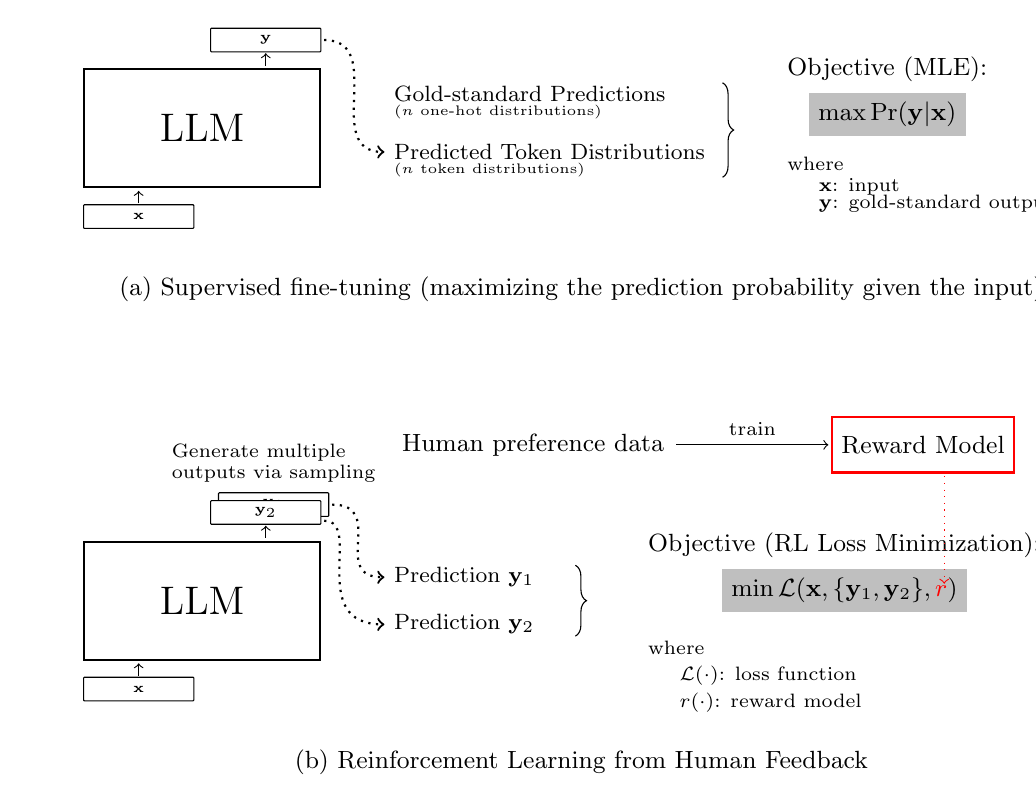
\begin{tikzpicture}
	
\def\ssep{1.9cm}

\tikzstyle{snode} = [minimum width=1.7cm,minimum height=0.8cm,inner sep=2pt,draw,thick,fill=white];
\tikzstyle{lnode} = [minimum width=3.0cm,minimum height=1.5cm,inner sep=2pt,draw,thick,fill=white];
\tikzstyle{cnode} = [minimum width=0.2cm,minimum height=0.2cm,inner sep=2pt,rounded corners=0.2mm];
\tikzstyle{dnode} = [minimum width=2.5cm,minimum height=0.7cm,inner sep=2pt,draw];
\tikzstyle{xnode} = [minimum width=1.4cm,minimum height=0.3cm,rounded corners=0.1mm,inner sep=1pt,draw,thin];

%%% sft
\begin{scope}

\node [lnode,anchor=west] (llm) at (0,0) {\Large{LLM}};
\node [xnode,anchor=north west] (inputx) at ([yshift=-0.2cm]llm.south west) {\tiny{$\mathbf{x}$}};
\node [xnode,anchor=south east] (outputy) at ([yshift=0.2cm]llm.north east) {\tiny{$\mathbf{y}$}};

\draw [->] ([yshift=0.01cm]inputx.north) -- ([yshift=0.17cm]inputx.north);
\draw [<-] ([yshift=-0.01cm]outputy.south) -- ([yshift=-0.17cm]outputy.south);


\node [anchor=west] (predicted) at ([xshift=0.8cm,yshift=-0.3cm]llm.east) {\footnotesize{Predicted Token Distributions}};
\node [anchor=north west] (predictedlabel) at ([yshift=0.2cm]predicted.south west) {\tiny{($n$ token distributions)}};

\node [anchor=south west] (gold) at ([yshift=0.3cm]predicted.north west) {\footnotesize{Gold-standard Predictions}};
\node [anchor=north west] (goldlabel) at ([yshift=0.2cm]gold.south west) {\tiny{($n$ one-hot distributions)}};

\draw [decoration={brace,amplitude=4pt},decorate] ([xshift=0.1cm,yshift=1.1cm]predicted.south east) -- ([xshift=0.1cm,yshift=-0.1cm]predicted.south east);

\node [anchor=west] (objective) at ([xshift=1.3cm,yshift=0.3cm]gold.east) {\small{Objective (MLE)}:};

\node [anchor=north,fill=gray!50] (objectivemath) at (objective.south) {\small{$\max \Pr(\mathbf{y}|\mathbf{x})$}};

\node [anchor=north west] (line1) at ([yshift=-0.7cm]objective.south west) {\scriptsize{where}};

\node [anchor=north west] (line2) at ([yshift=0.15cm,xshift=0.4cm]line1.south west) {\scriptsize{$\mathbf{x}$: input}};
\node [anchor=north west] (line3) at ([yshift=0.25cm]line2.south west) {\scriptsize{$\mathbf{y}$: gold-standard output}};

\draw [->,dotted,thick] ([xshift=1pt]outputy.east) .. controls +(east:0.8cm) and +(west:0.8cm) .. (predicted.west);

\node [anchor=north] (caption) at ([yshift=-1cm,xshift=3.3cm]llm.south east) {\small{(a) Supervised fine-tuning (maximizing the prediction probability given the input)}};

\end{scope}

%%% rlhf
\begin{scope}[yshift=-6cm]

\node [lnode,anchor=west] (llm) at (0,0) {\Large{LLM}};
\node [xnode,anchor=north west] (inputx) at ([yshift=-0.2cm]llm.south west) {\tiny{$\mathbf{x}$}};
\node [xnode,anchor=south east,fill=white] (outputy2) at ([yshift=0.3cm,xshift=0.1cm]llm.north east) {\tiny{$\mathbf{y}_1$}};
\node [xnode,anchor=south east,fill=white] (outputy) at ([yshift=0.2cm]llm.north east) {\tiny{$\mathbf{y}_2$}};
\node [anchor=south,align=left] (samplinglabel) at (outputy2.north) {\scriptsize{Generate multiple}\\[-0.15cm] \scriptsize{outputs via sampling}};

\draw [->] ([yshift=0.01cm]inputx.north) -- ([yshift=0.17cm]inputx.north);
\draw [<-] ([yshift=-0.01cm]outputy.south) -- ([yshift=-0.17cm]outputy.south);


\node [anchor=west] (predicted) at ([xshift=0.8cm,yshift=-0.3cm]llm.east) {\footnotesize{Prediction $\mathbf{y}_2$}};

\node [anchor=south west] (gold) at ([yshift=0.1cm]predicted.north west) {\footnotesize{Prediction $\mathbf{y}_1$}};

\draw [decoration={brace,amplitude=4pt},decorate] ([xshift=0.4cm,yshift=1.0cm]predicted.south east) -- ([xshift=0.4cm,yshift=0.1cm]predicted.south east);

%\node [anchor=west] (comparison) at ([xshift=0.5cm]predicted.north east) {$\mathbf{y}_a  \succ \mathbf{y}_b$};

\node [anchor=west] (objective) at ([xshift=1.2cm,yshift=0.4cm]gold.east) {\small{Objective (RL Loss Minimization)}:};

\node [anchor=north,fill=gray!50] (objectivemath) at (objective.south) {\small{$\min \mathcal{L}(\mathbf{x},\{\mathbf{y}_1,\mathbf{y}_2\},{\color{red} r})$}};
%\node [anchor=east,fill=red!30,inner sep=2pt] (rsymbol) at ([xshift=-0.3cm]objectivemath.east) {\small{$r$}};
%\draw [<-,dotted,red] ([yshift=1pt,xshift=-2pt]rsymbol.north) -- ([yshift=1.5cm-1pt,xshift=-2pt]rsymbol.north);

\node [anchor=south,minimum height=0.7cm,draw=red,thick] (rewardmodel) at ([yshift=1.2cm,xshift=1cm]objectivemath.north) {\small{Reward Model}};
\draw [->,dotted,red] ([xshift=-0.9cm,yshift=-1pt]rewardmodel.south east) -- ([xshift=-0.9cm,yshift=-1.4cm]rewardmodel.south east);

\node [anchor=east] (data) at ([xshift=-2.0cm]rewardmodel.west) {\small{Human preference data}};

\draw [->] ([xshift=1pt]data.east) -- ([xshift=-1pt]rewardmodel.west) node [pos=0.5,above] {\scriptsize{train}};

\node [anchor=north west] (line1) at ([yshift=-0.8cm]objective.south west) {\scriptsize{where}};

\node [anchor=north west] (line2) at ([yshift=0.10cm,xshift=0.4cm]line1.south west) {\scriptsize{$\mathcal{L}(\cdot)$: loss function}};
\node [anchor=north west] (line3) at ([yshift=0.15cm]line2.south west) {\scriptsize{$r(\cdot)$: reward model}};

\draw [->,dotted,thick] ([xshift=1pt,yshift=-3pt]outputy.east) .. controls +(east:0.5cm) and +(west:1.0cm) .. (predicted.west);
\draw [->,dotted,thick] ([xshift=1pt,yshift=-0pt]outputy2.east) .. controls +(east:0.7cm) and +(west:0.7cm) .. (gold.west);

\node [anchor=north] (caption) at ([yshift=-1cm,xshift=3.3cm]llm.south east) {\small{(b) Reinforcement Learning from Human Feedback}};

\end{scope}

\end{tikzpicture}
\end{center}

\caption{Supervised fine-tuning vs. reinforcement learning from human feedback. In supervised fine-tuning, we optimize the LLM by maximizing the probability of the prediction given the input. In reinforcement learning from human feedback, we first train a reward model on human preference data (on each pair of predictions, evaluators are asked to choose which one they prefer). Then, we use this reward model to supervise the LLM during fine-tuning.}
\label{fig:sft-vs-rlhf}
\end{figure}

\subsection{Basics of Reinforcement Learning}
\label{sec:rl-basics}

\noindent We begin by looking at some basic concepts of reinforcement learning. Note that the notation used here slightly differs from that used in the previous sections and chapters because we want to make our description more consistent with that in the reinforcement learning literature. Nevertheless, we will show how this notation corresponds to the language modeling notation. The reader who is already familiar with reinforcement learning techniques may skip or skim this subsection.

A general reinforcement learning framework describes how an agent interacts with a dynamic environment. This interaction is modeled as a sequence of actions taken by the agent in response to the state of the environment. At each time step, the agent observes the current state, chooses an action based on its policy, performs the action, and then receives feedback from the environment in the form of a reward and a new state. This observation-action-reward process is repeated until the agent achieves its goal.

A reinforcement learning system involves several components:

\begin{itemize}
\item \vspace{0.5em} \textbf{Agent}. This is the learner or decision-maker in reinforcement learning. In the context of LLMs, it can be seen as the LLM itself.
\item \vspace{0.3em} \textbf{Environment}. This includes everything external to the agent with which the agent interacts. But the environment in LLMs is less about a physical or virtual space and more about the framework within which the agent (e.g., an LLM) receives feedback and learns.
\item \vspace{0.3em} \textbf{State} ($s$). A state represents the current situation of the environment. Given a sequence of tokens for language modeling, a state at a time step can be viewed as the tokens we observed so far, that is, the context tokens we take to predict the next token. For example, we can define $(\mathbf{x}, \mathbf{y}_{< t})$ as the state when predicting the next token at time step $t$.
\item \vspace{0.3em} \textbf{Action} ($a$). Actions represent possible decisions the agent can make. In the context of LLMs, actions correspond to candidate tokens in the vocabulary.
\item \vspace{0.3em} \textbf{Reward} ($R$). The reward is the feedback from the environment that evaluates the success of an action. For example, $r(s,a,s')$ denotes the reward the agent receives for taking the action $a$ in state $s$ and moving to the next state $s'$. If the state-action sequence is given, we can denote the reward at the time step $t$ as $r_t = r(s_t,a_t,s_{t+1})$. Also note that if the decision-making process is deterministic, we can omit $s_{t+1}$ because it can be determined by $s_t$ and $a_t$. In such cases, we can use $r(s_t,a_t)$ as shorthand for $r(s_t,a_t,s_{t+1})$.
\item \vspace{0.3em} \textbf{Policy} ($\pi$). For an LLM, a policy is defined as the probability distribution over the tokens that the LLM predicts, given the preceding context tokens. Formally, this can be expressed as
    \begin{eqnarray}
    \pi(a|s) = \Pr(y_t|\mathbf{x}, \mathbf{y}_{< t}),
    \end{eqnarray}
    where $a$ corresponds to the token $y_t$, and $s$ corresponds to the context $(\mathbf{x}, \mathbf{y}_{< t})$. Figure \ref{fig:llm-as-policy-in-rl} illustrates how an LLM can be treated as a policy in the reinforcement learning framework.

\begin{figure}[!t]
\centering
% !Mode:: "TeX:UTF-8"
% !TEX encoding = UTF-8 Unicode

\begin{center}
\begin{tikzpicture}
	
\def\ssep{0.5cm}
\def\nsize{0.3cm}

\tikzstyle{lnode} = [minimum width=7cm,minimum height=1.1cm,inner sep=2pt,draw,thick,fill=white];

%%% step t
\begin{scope}

\node [anchor=west] (x0) at (0,0) {\scriptsize{$x_0$}};
\node [anchor=west] (x1) at ([xshift=\ssep]x0) {\scriptsize{$x_1$}};
\node [anchor=west] (x2) at ([xshift=\ssep]x1) {\scriptsize{$...$}};
\node [anchor=west] (x3) at ([xshift=\ssep]x2) {\scriptsize{$x_m$}};
\node [anchor=west] (y1) at ([xshift=\ssep]x3) {\scriptsize{$y_1$}};
\node [anchor=west] (y2) at ([xshift=\ssep]y1) {\scriptsize{$...$}};
\node [anchor=west] (y3) at ([xshift=\ssep]y2) {\scriptsize{$y_{t-1}$}};
%\node [anchor=west] (y4) at ([xshift=\ssep]y3) {\scriptsize{$y_{t}$}};
%\node [anchor=west] (y5) at ([xshift=\ssep]y4) {\scriptsize{$...$}};

\node [lnode,anchor=south] (llm) at ([xshift=0,yshift=0.3cm]y1.north) {\large{Policy (LLM)}};

\draw [->] ([yshift=0.18cm]x0.center) -- ([yshift=0.47cm]x0.center);
\draw [->] ([yshift=0.18cm]x1.center) -- ([yshift=0.47cm]x1.center);
\draw [->] ([yshift=0.18cm]x3.center) -- ([yshift=0.47cm]x3.center);
\draw [->] ([yshift=0.18cm]y1.center) -- ([yshift=0.47cm]y1.center);
\draw [->] ([yshift=0.18cm]y3.center) -- ([yshift=0.47cm]y3.center);
%\draw [->] ([yshift=0.18cm]y4.center) -- ([yshift=0.47cm]y4.center);

%\node [anchor=center] (ox0) at ([yshift=2.0cm]x0.north) {\scriptsize{\color{gray!50} $x_1$}};
%\node [anchor=center] (ox1) at ([yshift=2.0cm]x1.north) {\scriptsize{\color{gray!50} $x_2$}};
%\node [anchor=center] (ox2) at ([yshift=2.0cm]x2.north) {\scriptsize{\color{gray!50} $...$}};
\node [anchor=center] (ox3) at ([yshift=2.0cm]x3.north) {\scriptsize{\color{gray!50} $y_1$}};
\node [anchor=center] (oy1) at ([yshift=2.0cm]y1.north) {\scriptsize{\color{gray!50} $y_2$}};
\node [anchor=center] (oy2) at ([yshift=2.0cm]y2.north) {\scriptsize{\color{gray!50} $...$}};
\node [anchor=center] (oy3) at ([yshift=2.0cm]y3.north) {\scriptsize{$y_t$}};
%\node [anchor=center] (oy4) at ([yshift=2.0cm]y4.north) {\scriptsize{$y_{t+1}$}};
%\node [anchor=center] (oy5) at ([yshift=2.0cm]y5.north) {\scriptsize{$...$}};

%\draw [<-,gray!50] ([yshift=-0.18cm]ox0.center) -- ([yshift=-0.47cm]ox0.center);
%\draw [<-,gray!50] ([yshift=-0.18cm]ox1.center) -- ([yshift=-0.47cm]ox1.center);
\draw [<-,gray!50] ([yshift=-0.18cm]ox3.center) -- ([yshift=-0.47cm]ox3.center);
\draw [<-,gray!50] ([yshift=-0.18cm]oy1.center) -- ([yshift=-0.47cm]oy1.center);
\draw [<-] ([yshift=-0.18cm]oy3.center) -- ([yshift=-0.47cm]oy3.center);
%\draw [<-] ([yshift=-0.18cm]oy4.center) -- ([yshift=-0.47cm]oy4.center);

\draw [decoration={brace,amplitude=4pt},decorate] ([xshift=0,yshift=-0.2cm]y3.east) -- ([xshift=0,yshift=-0.2cm]x0.west) node [pos=0.5,below,yshift=-0.2cm,fill=lightsalmon!80] (statebox) {\scriptsize{State $s_t$ ($\mathbf{x}$ and $\mathbf{y}_{<t}$)}};

\node [anchor=south,fill=lightskyblue!80] (actionbox) at ([yshift=-0.0cm]oy3.north) {\scriptsize{Action $a_t$}};

\node [anchor=south west,minimum width=3.5cm,minimum height=1.3cm,draw,thick,align=center] (rewardmodel) at ([yshift=-1.4cm,xshift=2cm]llm.south east) {\footnotesize{Reward Model}\\[-0.1cm] \small{$R(\ $\ctext[RGB]{255,160,122}{$s_t$},\ \ctext[RGB]{135,206,250}{$a_t$}\ $)$}};

\node [anchor=south west,minimum width=3.5cm,minimum height=1.3cm,draw,thick,align=center] (valuefunction) at ([yshift=1.4cm]rewardmodel.north west) {\footnotesize{Value Functions}\\[-0.1cm] \small{$V($\ \ctext[RGB]{255,160,122}{$s_t$}\ $)$} \small{and} \small{$Q($\ \ctext[RGB]{255,160,122}{$s_t$},\ \ctext[RGB]{135,206,250}{$a_t$}\ $)$}};

\draw [->,thin] ([xshift=2pt]actionbox.east) -- ([xshift=2cm]actionbox.east) -- ([xshift=2cm,yshift=-3cm]actionbox.east) --  ([xshift=3cm,yshift=-3cm]actionbox.east);
\draw [->,thin] ([xshift=2pt]statebox.east) -- ([xshift=4.74cm]statebox.east);

\draw [->,thick] ([yshift=2pt]rewardmodel.north) -- ([yshift=-2pt]valuefunction.south);

\draw [->,thick,dotted] ([yshift=2pt]valuefunction.north) -- ([yshift=1.2cm]valuefunction.north) -- ([yshift=1.2cm,xshift=-5.6cm]valuefunction.north) node [pos=0.5,above] {\small{Feedback}} -- ([yshift=-0.17cm,xshift=-5.6cm]valuefunction.north);

\end{scope}

\end{tikzpicture}
\end{center}

\caption{LLM as policy in reinforcement learning. At each step $t$, the LLM predicts a token $y_t$ given the model input $\mathbf{x}$ and the previously generated tokens $\mathbf{y}_{<t}$. This process can be framed as a reinforcement learning problem, where $y_t$ serves as the action, $(\mathbf{x},\mathbf{y}_{<t})$ as the state, and the predicted distribution $\Pr(y_t|\mathbf{x},\mathbf{y}_{<t})$ as the policy. The reward model evaluates the generated response and assigns reward scores, which are then used to estimate value functions such as $V(s_t)$ and $Q(s_t,a_t)$ for policy optimization. In practice, reward models in RLHF are typically defined over complete responses, although the optimization objective can still be decomposed token-wise.}
\label{fig:llm-as-policy-in-rl}
\end{figure}

\item \vspace{0.3em} \textbf{Value Function} ($V$ and $Q$). A \mindex{state-value function} (or value function, for short) assesses the expected discounted return (i.e., accumulated rewards) for an agent starting from a particular state $s$ and following a specific policy $\pi$. It is defined as:
    \begin{eqnarray}
    V(s) & = & \mathbb{E} \Big[ r(s_0,a_0,s_1) + \gamma r(s_1,a_1,s_2) + \gamma^2 r(s_2,a_2,s_3) + \cdots \ \big | \ s_0 = s, \pi \Big] \nonumber \\
         & = & \mathbb{E} \Big[ r_0 + \gamma r_1 + \gamma^2 r_2 + \cdots \ \big | \ s_0 = s, \pi \Big] \nonumber \\
         & = & \mathbb{E} \Big[ \sum_{t=0}^{\infty} \gamma^{t} r_t \ \big | \ s_0 = s, \pi \Big], \label{eq:general-value-function}
    \end{eqnarray}
    \noindent where $\gamma \in [0,1]$ is the discount factor that adjusts the importance of future rewards, $s_0 = s$ indicates that the agent starts with the state $s$, and the expectation $\mathbb{E}$ is performed over all possible trajectories (i.e., state-action sequences). Similarly, an \mindex{action-value function} (or \mindex{Q-value function}) measures the expected return starting from a state $s$ taking an action $a$ and thereafter following a policy $\pi$, given by
    \begin{eqnarray}
    Q(s,a) & = & \mathbb{E} \Big[ \sum_{t=0}^{\infty} \gamma^{t} r_t \ \big | \ s_0 = s, a_0 = a, \pi \Big],
    \end{eqnarray}
    \noindent where $a_0 = a$ indicates that the action taken at the initial state is $a$.
\end{itemize}
\vspace{0.5em}

The goal of reinforcement learning is to learn a policy that maximizes the \mindex{cumulative reward} (or \mindex{return}) the agent receives over the long run. For simplicity, in the following derivations we omit the discount factor (i.e., $\gamma = 1$), unless otherwise specified.  Given a state-action sequence $\tau = \{(s_1,a_1),...,(s_T,a_T)\}$\footnote{We assume the state-action sequence begins with $s_1$ and $a_1$, rather than $s_0$ and $a_0$, to align with the notation commonly used in this chapter, where the prediction $\mathbf{y}$ typically starts from $y_1$. Of course, it is also common to denote a state-action sequence as $\{(s_0,a_0),...,(s_T,a_T)\}$ or $\{(s_0,a_0),...,(s_{T-1},a_{T-1})\}$ in the literature. But this variation in notation does not affect the discussion of the models presented here.}, the cumulative reward  over this sequence can be written as
\begin{eqnarray}
R(\tau) & = & \sum_{t=1}^{T} r_t. \label{eq:rl-sequence-reward}
\end{eqnarray}

The expectation of this cumulative reward over a space of state-action sequences is given in the form
\begin{eqnarray}
J(\theta) & = & \mathop{\mathbb{E}}_{\tau \sim \mathcal{T}} \Big[ R(\tau) \ \big | \pi_{\theta} \Big] \nonumber \\
          & = & \sum_{\tau \in \mathcal{T}} \mathrm{Pr}_{\theta}(\tau) R(\tau) \nonumber \\
          & = & \sum_{\tau \in \mathcal{T}} \mathrm{Pr}_{\theta}(\tau) \sum_{t=1}^{T} r_t, \label{eq:performance-function-basic}
\end{eqnarray}

\noindent where $\tau \sim \mathcal{T}$ indicates that $\tau$ is drawn from the state-action sequence space $\mathcal{T}$, and the subscript $\theta$ indicates the parameters of the policy. $J(\theta)$ is also called the \mindex{performance function}.

Then the training objective is to maximize $J(\theta)$:

\begin{eqnarray}
\tilde{\theta} & = & \argmax_{\theta} J(\theta). \label{eq:rl-optimize-j-theta}
\end{eqnarray}

Now, we have a simple reinforcement learning approach: 1) we sample a number of state-action sequences; then, 2) we evaluate each sequence using the performance function; then, 3) we update the model to maximize this performance function. If we take Eq. (\ref{eq:performance-function-basic}) and use gradient descent to optimize the policy, this constitutes a policy gradient method \cite{williams:1992simple}.

Note that in many NLP problems, such as machine translation, rewards are typically sparse. For instance, a reward is only received at the end of a complete sentence. This means that $r_t = 0$ for all $t < T$, and $r_t$ is non-zero only when $t = T$. Ideally, one might prefer feedback to be immediate and frequent (dense), and thus the training of the policy can be easier and more efficient. While several methods have been proposed to address sparse rewards, such as reward shaping, we will continue in our discussion to assume a sparse reward setup, where the reward is available only upon completing the prediction.

The model described in Eqs. (\ref{eq:rl-sequence-reward}-\ref{eq:rl-optimize-j-theta}) establishes a basic form of reinforcement learning, and many variants and improvements of this model have been developed. Before showing those more sophisticated models, let us take a moment to interpret the objective function $J(\theta)$ from the perspective of policy gradient. In gradient descent, we need to compute the gradient of $J(\theta)$ with respect to $\theta$:
\begin{eqnarray}
\frac{\partial J(\theta)}{\partial \theta} & = & \frac{\partial  \sum_{\tau \in \mathcal{T}} \mathrm{Pr}_{\theta}(\tau) R(\tau)}{\partial \theta} \nonumber \\
& = & \sum_{\tau \in \mathcal{T}} \frac{\partial  \mathrm{Pr}_{\theta}(\tau) }{\partial \theta}  R(\tau) \nonumber \\
& = & \sum_{\tau \in \mathcal{T}} \mathrm{Pr}_{\theta}(\tau) \frac{\partial  \mathrm{Pr}_{\theta}(\tau)/\partial \theta}{\mathrm{Pr}_{\theta}(\tau) } R(\tau) \nonumber \\
& = & \sum_{\tau \in \mathcal{T}} \mathrm{Pr}_{\theta}(\tau) \frac{\partial  \log \mathrm{Pr}_{\theta}(\tau) }{\partial \theta} R(\tau). \label{eq:rl-gradient-j-theta}
\end{eqnarray}

In practice, the expectation is often approximated using uniformly sampled trajectories from a batch (i.e., $\mathrm{Pr}_{\theta}(\tau) = 1/|\mathcal{T}|$).  In this case we can simplify Eq. (\ref{eq:rl-gradient-j-theta}) and need only consider the terms $\frac{\partial \log \mathrm{Pr}_{\theta}(\tau)}{\partial \theta}$ and $R(\tau)$:
\begin{eqnarray}
\frac{\partial J(\theta)}{\partial \theta} & = & \frac{1}{m} \sum_{\tau \in \mathcal{T}} \frac{\partial  \log \mathrm{Pr}_{\theta}(\tau)}{\partial \theta} R(\tau). \label{eq:rl-j-theta-gradient-simplified}
\end{eqnarray}

\noindent One advantage of this result is that $R(\tau)$ does not need to be differentiable, which means that we can use any type of reward function in reinforcement learning.

By treating the generation of the sequence $\tau$ as a Markov decision process, we can further derive $\frac{\partial \log \mathrm{Pr}_{\theta}(\tau)}{\partial \theta}$, and obtain:
\begin{eqnarray}
\frac{\partial \log \mathrm{Pr}_{\theta}(\tau)}{\partial \theta} & = & \frac{\partial}{\partial \theta} \log \prod_{t=1}^{T} \pi_{\theta}(a_t|s_t) \Pr(s_{t+1}|s_t,a_t) \nonumber \\
& = & \frac{\partial}{\partial \theta} \sum_{t=1}^{T} \underbrace{\log \pi_{\theta}(a_t|s_t)}_{\text{policy}} + \frac{\partial}{\partial \theta} \sum_{t=1}^{T} \underbrace{\log \Pr(s_{t+1}|s_t,a_t)}_{\text{dynamics}}, \label{eq:gradient-policy-and-dynamics}
\end{eqnarray}

\noindent where the gradient is decomposed into two parts: the policy gradient and the dynamics gradient. The policy component, $\log \pi_{\theta}(a_t|s_t)$, determines the log-probability of taking action $a_t$ given state $s_t$, and it is parameterized by $\theta$. The dynamics component, $\log \Pr(s_{t+1}|s_t,a_t)$, represents the log-probability of transitioning to state $s_{t+1}$ from state $s_t$ after taking action $a_t$. In typical reinforcement learning settings, the dynamics are not directly influenced by the policy parameters $\theta$, and thus, their derivatives are often zero. In this case, therefore, Eq. (\ref{eq:gradient-policy-and-dynamics}) can be simplified to:
\begin{eqnarray}
\frac{\partial \log \mathrm{Pr}_{\theta}(\tau)}{\partial \theta} & = & \frac{\partial}{\partial \theta} \sum_{t=1}^{T} \log \pi_{\theta}(a_t|s_t). \label{eq:rl-policy-gradient-product-of-pi}
\end{eqnarray}

\noindent In other words, we only concentrate on optimizing the policy without concerning ourselves with the underlying dynamics.

Substituting Eq. (\ref{eq:rl-policy-gradient-product-of-pi}) into Eq. (\ref{eq:rl-j-theta-gradient-simplified}), and expanding $R(\tau)$, we then obtain
\begin{eqnarray}
\frac{\partial J(\theta)}{\partial \theta} & = & \frac{1}{|\mathcal{T}|} \sum_{\tau \in \mathcal{T}} \frac{\partial}{\partial \theta} \Big( \sum_{t=1}^{T} \log \pi_{\theta}(a_t|s_t) \sum_{t=1}^{T} r_t \Big).
\end{eqnarray}

While this policy gradient approach is straightforward, it suffers from the problem that the variance of the estimated gradients can be very high, making the learning process noisy and inefficient. One reason for this high variance problem is that rewards can vary greatly across different steps or scenarios. Imagine that in a sequence of action decisions, the reward model tends to assign small rewards to good actions (e.g., $R_t = 2$) and large penalties to poor actions (e.g., $R_t = -50$). Such varying reward scales for good and poor actions can result in a very low total reward for the entire sequence, even if it includes good actions.

One simple method for reducing the variance of the gradient is to set a baseline $b$ and subtract it from $\sum_{t=1}^{T} r_t$, resulting in $\sum_{t=1}^{T} r_t - b$.\footnote{In fact, the use of a baseline $b$ does not change the variance of the total rewards $\sum_{t=1}^{T} r_t$. However, it is important to note that while introducing a baseline does not alter the overall variance of the rewards, it helps reduce the variance of the gradient estimates. In general, the operation $\sum_{t=1}^{T} r_t - b$ centers the rewards around zero (e.g., $b$ is defined as the expected value of $\sum_{t=1}^{T} r_t$), which can lead to reduced variance in the product $\sum_{t=1}^{T} \log \pi_{\theta}(a_t|s_t) (\sum_{t=1}^{T} r_t - b)$.} Here, the baseline can be interpreted as a reference point. By centering the rewards around this baseline, we remove systematic biases in the reward signal, making the updates more stable and less sensitive to extreme fluctuations in individual rewards.

This policy gradient model with a baseline can be given by
\begin{eqnarray}
\frac{\partial J(\theta)}{\partial \theta} & = & \frac{1}{|\mathcal{T}|} \sum_{\tau \in \mathcal{T}} \frac{\partial}{\partial \theta} \Big( \sum_{t=1}^{T} \log \pi_{\theta}(a_t|s_t) \Big) \Big(\sum_{t=1}^{T} r_t - b \Big) \nonumber \\
& = & \frac{1}{|\mathcal{T}|} \sum_{\tau \in \mathcal{T}} \frac{\partial}{\partial \theta} \Big[ \sum_{t=1}^{T} \log \pi_{\theta}(a_t|s_t) \Big(\sum_{k=1}^{T} r_k - b \Big) \Big] \nonumber \\
& = & \frac{1}{|\mathcal{T}|} \sum_{\tau \in \mathcal{T}} \frac{\partial}{\partial \theta} \Big[ \sum_{t=1}^{T} \log \pi_{\theta}(a_t|s_t) \Big(\sum_{k=1}^{t-1} r_k + \sum_{k=t}^{T} r_k - b \Big) \Big]. \label{eq:policy-gradient-with-baseline}
\end{eqnarray}

\noindent Here we write $\sum_{k=1}^{T} r_k$ as the sum of two terms $\sum_{k=1}^{t-1} r_k$ and $\sum_{k=t}^{T} r_k$ to distinguish between the rewards accrued before and after the action at time step $t$. Note that rewards received before time step $t$ do not depend on the action taken at time step $t$. Therefore, the term $\sum_{k=1}^{t-1} r_k$ does not contribute to the gradient and can be omitted. This leads to a simplified version of Eq. (\ref{eq:policy-gradient-with-baseline})
\begin{eqnarray}
\frac{\partial J(\theta)}{\partial \theta} & = & \frac{1}{|\mathcal{T}|} \sum_{\tau \in \mathcal{T}} \frac{\partial}{\partial \theta} \Big[ \sum_{t=1}^{T} \log \pi_{\theta}(a_t|s_t) \Big(\sum_{k=t}^{T} r_k - b \Big) \Big].
\end{eqnarray}

\noindent Also note that removing $\sum_{k=1}^{t-1} r_k$ can further reduce the variance of the gradient.

There are many ways to define the baseline $b$. Here we consider the value function of the state $s_t$, that is, the estimated value of being in state $s_t$: $V(s_t) = \mathbb{E}(r_t + r_{t+1} + \cdots + r_{T})$. Hence we have
\begin{eqnarray}
A(s_t,a_t) & = & \sum_{k=t}^{T} r_k - b \nonumber \\
           & = & \sum_{k=t}^{T} r_k - V(s_t),
\end{eqnarray}

\noindent where $\sum_{k=t}^{T} r_k $ represents the actual return received, and $V(s_t)$ represents the expected return. $A(s_t,a_t)$ (or $A_t$ for short) is called the \mindex{advantage} at time step $t$, which quantifies the relative benefit of the action $a_t$ compared to the expected value of following the policy from the state $s_t$ onward.

By using the advantage function $A(s_t,a_t)$, the gradient of $J(\theta)$ can be written in the form
\begin{eqnarray}
\frac{\partial J(\theta)}{\partial \theta} & = & \frac{1}{|\mathcal{T}|} \sum_{\tau \in \mathcal{T}} \frac{\partial}{\partial \theta} \Big( \sum_{t=1}^{T} \log \pi_{\theta}(a_t|s_t) A(s_t,a_t) \Big). \label{eq:a2c-policy-gradient}
\end{eqnarray}

This objective forms the basis of \mindex{advantage actor-critic} (\mindex{A2C}) methods in reinforcement learning \cite{mnih-etal:2016asynchronous}. In this method, the actor aims at learning a policy. It updates the policy parameters using Eq. (\ref{eq:a2c-policy-gradient}) to help focus more on actions that are likely to improve performance. The critic, on the other hand, updates its estimation of the value function, which is used to calculate the advantage function $A(s_t,a_t)$, thus serving as the evaluator of the policy being learned by the actor.

In the A2C method, $A(s_t,a_t)$ is typically expressed as the difference of the action-value function $Q(s_t,a_t)$ and the state-value function $V(s_t)$:
\begin{eqnarray}
A(s_t,a_t) & = & Q(s_t,a_t) - V(s_t). \label{eq:advantage-q-v}
\end{eqnarray}

\noindent At first glance, this model may seem challenging to develop because it requires two separate sub-models to calculate $Q(s_t,a_t)$ and $V(s_t)$, respectively. Fortunately, considering that $Q(s_t,a_t)$ can be defined as the return $r_t + V(s_{t+1})$, we can rewrite Eq. (\ref{eq:advantage-q-v}) as
\begin{eqnarray}
A(s_t,a_t) & = & r_t + V(s_{t+1}) - V(s_t),
\end{eqnarray}

\noindent or alternatively, introduce the discount factor $\gamma$ to obtain a more general form
\begin{eqnarray}
A(s_t,a_t) & = & r_t + \gamma V(s_{t+1}) - V(s_t).
\end{eqnarray}

\noindent $A(s_t,a_t) = r_t + \gamma V(s_{t+1}) - V(s_t)$ is also called the \mindex{temporal difference} (\mindex{TD}) error. What we need is to train a critic network for the value function $V(s_t)$, and then use it to compute the advantage function\footnote{The training loss for the value network (or critic network) in A2C is generally formulated as the mean squared error between the computed return $r_t + \gamma V(s_{t+1})$ and the predicted state value $V(s_t)$. Suppose that the value network is parameterized by $\omega$. The loss function is given by
\begin{eqnarray}
\mathcal{L}_v(\omega) & = & \frac{1}{M} \sum \big(r_t + \gamma V_{\omega}(s_{t+1}) - V_{\omega}(s_t) \big)^2,
\end{eqnarray}

\noindent where $M$ is the number of training samples, for example, for a sequence of $T$ tokens, we can set $M=T$.
}.

Up to this point, we have spent considerable space discussing the basics of reinforcement learning, especially on how to derive the optimization objective for the A2C method. However, reinforcement learning is a vast field, and many technical details cannot be covered here. The interested reader can refer to reinforcement learning books for more details \cite{Sutton-and-Barto:2018RL,szepesvari:2010algorithms}. Nevertheless, we now have the necessary knowledge to further discuss RLHF. In the subsequent subsections, we will return to the discussion on LLM alignment, demonstrating how to use the A2C method for aligning with human preferences.

\subsection{Training Reward Models}
\label{sec:training-reward-models}

\noindent We have shown that reward models play a very important role in the general reinforcement learning framework and form the basis for computing value functions. We now consider the problem of training these reward models.

In RLHF, a reward model is a neural network that maps a pair of input and output token sequences to a scalar reward score. Given an input $\mathbf{x}$ and an output $\mathbf{y}$, the reward can be expressed as
\begin{eqnarray}
r & = & \mathrm{Reward}(\mathbf{x},\mathbf{y}),
\end{eqnarray}

\noindent where $\mathrm{Reward}(\cdot)$ is the reward model. $r$ can be interpreted as a measure of how well the output $\mathbf{y}$ aligns with the desired behavior given the input $\mathbf{x}$. As discussed in the previous subsection, both $\mathbf{x}$ and $\mathbf{y}$ are assumed to be complete token sequences. As a result, the reward model evaluates the quality of a fully generated output conditioned on the input, rather than assigning rewards to intermediate generation steps. For example, during sequence generation, the reward is typically provided only at the final position of the output sequence $\mathbf{y}=y_1...y_n$. To keep the notation uncluttered, we will use $r(\mathbf{x},\mathbf{y})$ to denote the reward model $\mathrm{Reward}(\mathbf{x},\mathbf{y})$ from here on.

There are many ways to implement the reward model. One simple approach is to build the reward model based on a pre-trained LLM. More specifically, we can concatenate $\mathbf{x}$ and $\mathbf{y}$ to form a single token sequence $\mathrm{seq}_{\mathbf{x},\mathbf{y}} = [\mathbf{x}, \mathbf{y}]$. We run a pre-trained LLM on this sequence, as usual, and at each position, we obtain a representation from the last Transformer layer. Then, we take the representation at the last position (denoted by $\mathbf{h}_{\mathrm{last}}$) and map it to a scalar via a linear transformation:
\begin{eqnarray}
r(\mathbf{x},\mathbf{y}) & = & \mathbf{h}_{\mathrm{last}} \mathbf{W}_{r},
\end{eqnarray}

\noindent where $\mathbf{h}_{\mathrm{last}}$ is a $d$-dimensional vector, and $\mathbf{W}_{r}$ is a $d \times 1$ linear mapping matrix. This architecture of the reward model is illustrated in Figure \ref{fig:reward-model-architecture}.

\begin{figure}[!t]
\centering
% !Mode:: "TeX:UTF-8"
% !TEX encoding = UTF-8 Unicode

\begin{center}
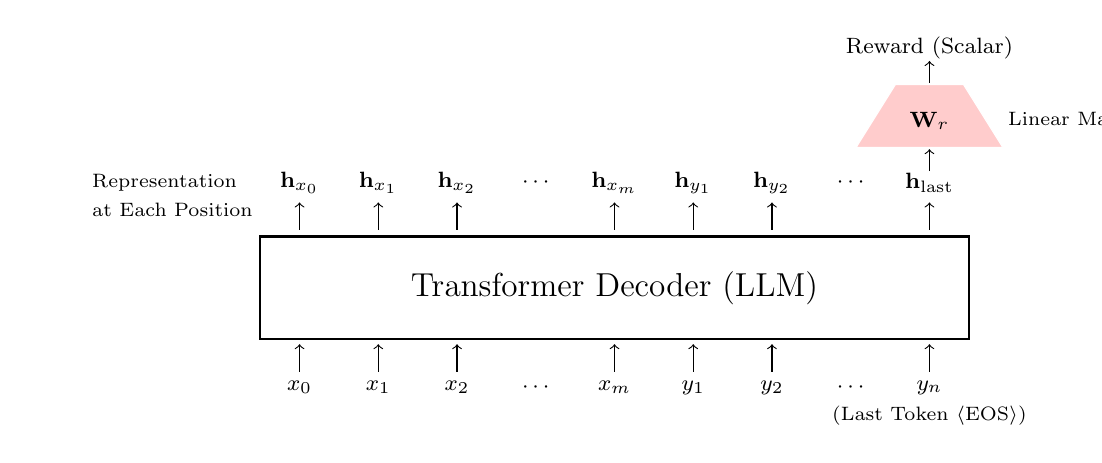
\begin{tikzpicture}
	
\def\ssep{1cm}
\def\nsize{0.3cm}

\tikzstyle{lnode} = [minimum width=7cm,minimum height=1.1cm,inner sep=2pt,draw,thick,fill=white];

\begin{scope}

\node [anchor=west] (x0) at (0,0) {\footnotesize{$x_0$}};
\node [anchor=center] (x1) at ([xshift=\ssep]x0.center) {\footnotesize{$x_1$}};
\node [anchor=center] (x2) at ([xshift=\ssep]x1.center) {\footnotesize{$x_2$}};
\node [anchor=center] (x3) at ([xshift=\ssep]x2.center) {\footnotesize{$\cdots$}};
\node [anchor=center] (x4) at ([xshift=\ssep]x3.center) {\footnotesize{$x_m$}};
\node [anchor=center] (y1) at ([xshift=\ssep]x4.center) {\footnotesize{$y_1$}};
\node [anchor=center] (y2) at ([xshift=\ssep]y1.center) {\footnotesize{$y_2$}};
\node [anchor=center] (y3) at ([xshift=\ssep]y2.center) {\footnotesize{$\cdots$}};
\node [anchor=center] (y4) at ([xshift=\ssep]y3.center) {\footnotesize{$y_n$}};
\node [anchor=north] (y4label) at ([yshift=0.1cm]y4.south) {\scriptsize{(Last Token $\langle \mathrm{EOS} \rangle$)}};

\draw [->] ([yshift=0.2cm]x0.center) -- ([yshift=0.55cm]x0.center);
\draw [->] ([yshift=0.2cm]x1.center) -- ([yshift=0.55cm]x1.center);
\draw [->] ([yshift=0.2cm]x2.center) -- ([yshift=0.55cm]x2.center);
\draw [->] ([yshift=0.2cm]x4.center) -- ([yshift=0.55cm]x4.center);
\draw [->] ([yshift=0.2cm]y1.center) -- ([yshift=0.55cm]y1.center);
\draw [->] ([yshift=0.2cm]y2.center) -- ([yshift=0.55cm]y2.center);
\draw [->] ([yshift=0.2cm]y4.center) -- ([yshift=0.55cm]y4.center);

\node [anchor=center] (ox0) at ([yshift=2.6cm]x0.center) {\footnotesize{$\mathbf{h}_{x_0}$}};
\node [anchor=center] (ox1) at ([yshift=2.6cm]x1.center) {\footnotesize{$\mathbf{h}_{x_1}$}};
\node [anchor=center] (ox2) at ([yshift=2.6cm]x2.center) {\footnotesize{$\mathbf{h}_{x_2}$}};
\node [anchor=center] (ox3) at ([yshift=2.6cm]x3.center) {\footnotesize{$\cdots$}};
\node [anchor=center] (ox4) at ([yshift=2.6cm]x4.center) {\footnotesize{$\mathbf{h}_{x_m}$}};
\node [anchor=center] (oy1) at ([yshift=2.6cm]y1.center) {\footnotesize{$\mathbf{h}_{y_1}$}};
\node [anchor=center] (oy2) at ([yshift=2.6cm]y2.center) {\footnotesize{$\mathbf{h}_{y_2}$}};
\node [anchor=center] (oy3) at ([yshift=2.6cm]y3.center) {\footnotesize{$\cdots$}};
\node [anchor=center] (oy4) at ([yshift=2.6cm]y4.center) {\footnotesize{$\mathbf{h}_{\mathrm{last}}$}};

\node [anchor=south,draw,thick,minimum width=9cm,minimum height=1.3cm] (llm) at ([yshift=0.4cm]x4.north) {\large{Transformer Decoder (LLM)}};
\node [anchor=east] (representation) at ([xshift=-0.3cm]ox0.west) {\scriptsize{Representation}};
\node [anchor=north west] (representation2) at ([yshift=0.1cm]representation.south west) {\scriptsize{at Each Position}};

\draw [<-] ([yshift=-0.25cm]ox0.center) -- ([yshift=-0.6cm]ox0.center);
\draw [<-] ([yshift=-0.25cm]ox1.center) -- ([yshift=-0.6cm]ox1.center);
\draw [<-] ([yshift=-0.25cm]ox2.center) -- ([yshift=-0.6cm]ox2.center);
\draw [<-] ([yshift=-0.25cm]ox4.center) -- ([yshift=-0.6cm]ox4.center);
\draw [<-] ([yshift=-0.25cm]oy1.center) -- ([yshift=-0.6cm]oy1.center);
\draw [<-] ([yshift=-0.25cm]oy2.center) -- ([yshift=-0.6cm]oy2.center);
\draw [<-] ([yshift=-0.25cm]oy4.center) -- ([yshift=-0.6cm]oy4.center);

\filldraw [fill=red!20,draw=white] ([xshift=-0.5cm,yshift=0.2cm]oy4.north west) -- ([xshift=0.5cm,yshift=0.2cm]oy4.north east) -- ([yshift=1cm,xshift=0]oy4.north east) -- ([yshift=1cm,xshift=0]oy4.north west) -- ([xshift=-0.5cm,yshift=0.2cm]oy4.north west);

\node [anchor=south] (reward) at ([yshift=1.2cm]oy4.north) {\footnotesize{Reward (Scalar)}};
\node [anchor=south] (Wr) at ([yshift=0.3cm]oy4.north) {\footnotesize{$\mathbf{W}_r$}};
\node [anchor=west] (linear) at ([xshift=0.5cm]Wr.east) {\scriptsize{Linear Map}};

\draw [->] ([yshift=-0.1cm]oy4.north) -- ([yshift=0.18cm]oy4.north);
\draw [<-] ([yshift=0.1cm]reward.south) -- ([yshift=-0.18cm]reward.south);

\end{scope}

\end{tikzpicture}
\end{center}

\caption{Architecture of a Transformer-based reward model. The main component of this model is still an LLM. We use the Transformer decoder as the sequence representation model. We take the representation at the last position of the decoder as the representation of the entire sequence $[\mathbf{x},\mathbf{y}]$. We then map this representation to a scalar through a linear transformation, which serves as the reward score for $[\mathbf{x},\mathbf{y}]$.}
\label{fig:reward-model-architecture}
\end{figure}

To train the reward model, the first step is to collect human feedback on a set of generated outputs. Given an input $\mathbf{x}$, we use the LLM to produce multiple candidate outputs $\{\mathbf{y}_1,...,\mathbf{y}_N\}$. Human feedback can be obtained in several ways:

\begin{itemize}
\item \vspace{0.5cm} \textbf{Pairwise Comparison} (\textbf{Pairwise Ranking}). Given two different outputs, human experts select which one is better.
\item \vspace{0.3cm} \textbf{Rating}. Human experts provide a score or rating to each output. This score is often a continuous or discrete numerical value, such as a score on a scale (e.g., 1-5 stars, or 1-10 points). In some cases, the rating might be binary, indicating a ``yes/no'' or ``positive/negative'' preference.
\item \vspace{0.3em} \textbf{Listwise Ranking}. Human experts are asked to rank or order the given set of possible outputs.
\end{itemize}
\vspace{0.5em}

Here we consider pairwise comparison feedback as it is one of the simplest and most common forms of human feedback used in RLHF.  In this setting, for each comparison, two outputs $(\mathbf{y}_a,\mathbf{y}_b)$ are randomly drawn from the candidate pool $\{\mathbf{y}_1,...,\mathbf{y}_N\}$. Human experts are then presented with these pairs and asked to decide which output they prefer based on criteria such as clarity, relevance, and accuracy. The human feedback can be encoded as a binary label. For example, $\mathbf{y}_a \succ \mathbf{y}_b$ indicates a preference for $\mathbf{y}_a$, and $\mathbf{y}_b \succ \mathbf{y}_a$ indicates a preference for $\mathbf{y}_b$.

One simple and widely used model for describing such pairwise comparisons is the \mindex{Bradley-Terry model} \cite{bradley-and-terry:rank}. It is a probabilistic model that estimates the probability that one item is preferred over another. Adapting this model to the notation used here, we can write the probability that $\mathbf{y}_a$ is preferred over $\mathbf{y}_b$ in the form
\begin{eqnarray}
\Pr(\mathbf{y}_a \succ \mathbf{y}_b | \mathbf{x}) & = & \frac{e^{r(\mathbf{x},\mathbf{y}_a)}}{e^{r(\mathbf{x},\mathbf{y}_a)} + e^{r(\mathbf{x},\mathbf{y}_b)}} \nonumber \\
                                                  & = & \frac{e^{r(\mathbf{x},\mathbf{y}_a)-r(\mathbf{x},\mathbf{y}_b)}}{e^{r(\mathbf{x},\mathbf{y}_a)-r(\mathbf{x},\mathbf{y}_b)}+1} \nonumber \\
                                                  & = & \mathrm{Sigmoid}(r(\mathbf{x},\mathbf{y}_a)-r(\mathbf{x},\mathbf{y}_b)).
\end{eqnarray}

When training the reward model, our objective is to maximize this preference probability. A loss function based on the Bradley-Terry model is given by
\begin{eqnarray}
\mathcal{L}_r(\phi) & = & -\mathbb{E}_{(\mathbf{x},\mathbf{y}_a,\mathbf{y}_b) \sim \mathcal{D}_r} \big[ \log \mathrm{Pr}_{\phi}(\mathbf{y}_a \succ \mathbf{y}_b | \mathbf{x}) \big], \label{eq:pairwise-reward-loss-expectation}
\end{eqnarray}

\noindent where $(\mathbf{x},\mathbf{y}_a,\mathbf{y}_b)$ is drawn from a human-annotated dataset $\mathcal{D}_r$ consisting of preference pairs of outputs and their corresponding inputs. $\phi$ represents the parameters of the reward model, which includes both the parameters of the Transformer decoder and the linear mapping matrix $\mathbf{W}_r$. In practice, assuming $(\mathbf{x},\mathbf{y}_a,\mathbf{y}_b)$ is uniformly sampled from $\mathcal{D}_r$, the expectation can be approximated by the empirical average
\begin{eqnarray}
\mathcal{L}_r(\phi) & = & -\frac{1}{|\mathcal{D}_r|} \sum_{(\mathbf{x},\mathbf{y}_a,\mathbf{y}_b) \in \mathcal{D}_r} \log \mathrm{Pr}_{\phi}(\mathbf{y}_a \succ \mathbf{y}_b | \mathbf{x}). \label{eq:pairwise-reward-loss-sum}
\end{eqnarray}

The goal of training the reward model is to find the optimal parameters $\hat{\phi}$ that minimize this loss function, given by
\begin{eqnarray}
\hat{\phi} & = & \argmin_{\phi} \mathcal{L}_r(\phi).
\end{eqnarray}

\noindent Since the reward model itself is also an LLM, we can simply use the Transformer training procedure to optimize the reward model. The difference from training a standard LLM is that we only need to replace the cross-entropy loss with the pairwise comparison loss as described in Eq. (\ref{eq:pairwise-reward-loss-sum}). After training the reward model, we can apply the trained reward model $r_{\hat{\phi}}(\cdot)$ to supervise the target LLM for alignment.

It is worth noting that although we train the reward model to perform pairwise ranking, we apply it to score each input-output pair independently during the alignment process. The pairwise ranking objective ensures that the reward model is sensitive to subtle differences between outputs, but we rely on the continuous scores produced by the reward model to guide the optimization of the LLM. An advantage of this approach is that we can choose from or combine various ranking loss functions, and still apply the resulting reward models in the same way as we have done in this subsection. This flexibility makes the reward modeling framework broadly applicable across different forms of human preference supervision.

\subsection{Training LLMs}
\label{sec:rlhf-training-llms}

\noindent Having obtained the reward model, we then train the policy (i.e., the LLM) via the A2C method. Recall from Section \ref{sec:rl-basics} that a state-action sequence or trajectory $\tau$ can be evaluated by the utility function
\begin{eqnarray}
U(\tau;\theta) & = &  \sum_{t=1}^{T} \log \pi_{\theta}(a_t|s_t) A(s_t,a_t), \label{eq:utility-basic-form}
\end{eqnarray}

\noindent where $A(s_t,a_t)$ is the advantage of taking the action $a_t$ given the state $s_t$. An estimate of $A(s_t,a_t)$ is defined as the TD error $ r_t + \gamma V(s_{t+1}) - V(s_t)$, where the value function $V(s_t)$ is trained with the reward model.

Given this utility function, the A2C-based loss function can be written in the form
\begin{eqnarray}
\mathcal{L}(\theta) & = & -\mathbb{E}_{\tau \sim \mathcal{T}} \big[U(\tau;\theta) \big] \nonumber \\
          & = & -\mathbb{E}_{\tau \sim \mathcal{T}} \big[ \sum_{t=1}^{T} \log \pi_{\theta}(a_t|s_t) A(s_t,a_t) \big],
\end{eqnarray}

\noindent where $\mathcal{T}$ is a space of state-action sequences. As usual, the goal of training the policy is to minimize this loss function
\begin{eqnarray}
\tilde{\theta} & = & \argmin_{\theta} \mathcal{L}(\theta).
\end{eqnarray}

If we map the problem back to the language modeling problem and adopt the notation from LLMs, the loss function can be written as:
\begin{eqnarray}
\mathcal{L}(\theta) & = & -\mathbb{E}_{(\mathbf{x},\mathbf{y}) \sim \mathcal{D}} \big[ U(\mathbf{x},\mathbf{y};\theta) \big],
\end{eqnarray}

\noindent where
\begin{eqnarray}
U(\mathbf{x},\mathbf{y};\theta) & = & \sum_{t=1}^{T} \log \pi_{\theta}(y_t|\mathbf{x},\mathbf{y}_{<t}) A(\mathbf{x},\mathbf{y}_{<t},y_t).
\end{eqnarray}

\noindent Here $\mathcal{D}$ is a set of input-output pairs, and $\pi_{\theta}(y_t|\mathbf{x},\mathbf{y}_{<t}) = \mathrm{Pr}_{\theta}(y_t|\mathbf{x},\mathbf{y}_{<t})$ is the LLM parameterized by $\theta$.

In general, we do not have a human annotated input-output dataset $\mathcal{D}$ in RLHF, but a dataset containing inputs only. The outputs, in this case, are typically the predictions made by the LLM. The loss function is then defined as
\begin{eqnarray}
\mathcal{L}(\theta) & = & -\mathbb{E}_{\mathbf{x} \sim \mathcal{D}} \mathbb{E}_{\mathbf{y} \sim \pi_{\theta}(\cdot|\mathbf{x})} \big[ U(\mathbf{x},\mathbf{y};\theta) \big],
\end{eqnarray}

\noindent where $\mathcal{D}$ denotes the input-only dataset, and $\mathbf{y} \sim \pi_{\theta}(\cdot|\mathbf{x})$ denotes that the output $\mathbf{y}$ is sampled by the policy $\pi_{\theta}(\cdot|\mathbf{x})$.

The above formulation provides a basic form of the A2C method for LLMs. Improved versions of this model are more commonly used in RLHF. In the following discussion, we will still use the reinforcement learning notation to simplify the presentation and will get back to the language modeling notation later.

One common improvement of policy gradient methods is to construct a surrogate objective using \mindex{importance sampling}. The resulting objective can be written as
\begin{eqnarray}
U(\tau;\theta) & = &  \sum_{t=1}^{T} \frac{\pi_{\theta}(a_t|s_t)}{\pi_{\theta_{\mathrm{ref}}}(a_t|s_t)} A(s_t,a_t).
\end{eqnarray}

\noindent Here we replace the log-probability $\log \pi_{\theta}(a_t|s_t)$ with the ratio $\frac{\pi_{\theta}(a_t|s_t)}{\pi_{\theta_{\mathrm{ref}}}(a_t|s_t)}$. $\theta_{\mathrm{ref}}$ denotes the parameters of the previous policy (such as an initial model from which we start the training). So $\frac{\pi_{\theta}(a_t|s_t)}{\pi_{\theta_{\mathrm{ref}}}(a_t|s_t)}$, also called the \mindex{ratio function}, can be interpreted as the probability ratio between the current policy $\pi_{\theta}$ and the reference policy $\pi_{\theta_{\mathrm{ref}}}$ (call it the reference policy). By using the ratio function we reweight the observed rewards based on the likelihood of the actions under the current policy versus the reference policy. When $\frac{\pi_{\theta}(a_t|s_t)}{\pi_{\theta_{\mathrm{ref}}}(a_t|s_t)} > 1$, the action $a_t$ is more favored by the current policy compared to the reference policy. By contrast, when $\frac{\pi_{\theta}(a_t|s_t)}{\pi_{\theta_{\mathrm{ref}}}(a_t|s_t)} < 1$, the action $a_t$ is less favored by the current policy\footnote{
Consider a more general case where we wish to evaluate the policy using its expected reward (also see Eq. (\ref{eq:performance-function-basic}))
\begin{eqnarray}
J(\theta) & = & \mathbb{E}_{\tau \sim \pi_{\theta}} \Big[ R(\tau) \Big].
\end{eqnarray}

\noindent Here $\tau \sim \pi_{\theta}$ means that the sequence $\tau$ is generated by the policy $\pi_{\theta}$. Alternatively, we can write $J(\theta)$ in another form
\begin{eqnarray}
J(\theta) & = & \mathbb{E}_{\tau \sim \pi_{\theta_{\mathrm{ref}}}} \Big[ \frac{\mathrm{Pr}_{\theta}(\tau)}{\mathrm{Pr}_{\theta_{\mathrm{ref}}}(\tau)} R(\tau) \Big]. \label{eq:importance-sampling-sequence-reward}
\end{eqnarray}

It is straightforward to see that the right-hand sides of these equations are essentially the same since $\mathbb{E}_{\tau \sim \pi_{\theta_{\mathrm{ref}}}} \Big[ \frac{\mathrm{Pr}_{\theta}(\tau)}{\mathrm{Pr}_{\theta_{\mathrm{ref}}}(\tau)} R(\tau) \Big] = \sum_{\tau} \mathrm{Pr}_{\theta_{\mathrm{ref}}}(\tau) \frac{\mathrm{Pr}_{\theta}(\tau)}{\mathrm{Pr}_{\theta_{\mathrm{ref}}}(\tau)} R(\tau) = \sum_{\tau} \mathrm{Pr}_{\theta}(\tau) R(\tau) = \mathbb{E}_{\tau \sim \pi_{\theta}} \Big[ R(\tau) \Big]$.

Note that this equivalence holds only when the expectation is performed over the entire sequence space. In practice, however, we often only sample a relatively small number of sequences using a policy in policy learning. As a result, the sampling method itself matters. Eq. (\ref{eq:importance-sampling-sequence-reward}) offers an interesting manner to separate the sampling and reward computation processes: we first use a baseline policy (with $\theta_{\mathrm{ref}}$) to sample a number of sequences, and then use the target policy (with $\theta$) to compute the expected reward. In this way, we separate the policy used for collecting the data, and the policy used for computing the gradient. This approach avoids the need to directly sample from the policy we are evaluating, which can be beneficial in cases where generating sequences from the target policy is expensive or difficult. In reinforcement learning, $\mathbb{E}_{\tau \sim \pi_{\theta_{\mathrm{ref}}}} \Big[ \frac{\mathrm{Pr}_{\theta}(\tau)}{\mathrm{Pr}_{\theta_{\mathrm{ref}}}(\tau)} R(\tau) \Big]$ is often called a \mindex{surrogate objective}.

Eq. (\ref{eq:importance-sampling-sequence-reward}) can also be interpreted from a policy gradient perspective. For $\mathbb{E}_{\tau \sim \pi_{\theta_{\mathrm{ref}}}} \Big[ \frac{\mathrm{Pr}_{\theta}(\tau)}{\mathrm{Pr}_{\theta_{\mathrm{ref}}}(\tau)} R(\tau) \Big]$, the gradient at $\theta=\theta_{\mathrm{ref}}$ is given by
\begin{eqnarray}
\frac{\partial}{\partial \theta} \mathbb{E}_{\tau \sim \pi_{\theta_{\mathrm{ref}}}} \Big[ \frac{\mathrm{Pr}_{\theta}(\tau)}{\mathrm{Pr}_{\theta_{\mathrm{ref}}}(\tau)} R(\tau) \Big] \Big |_{\theta = \theta_{\mathrm{ref}}} & = & \mathbb{E}_{\tau \sim \pi_{\theta_{\mathrm{ref}}}} \Big[ \frac{\partial \mathrm{Pr}_{\theta}(\tau) |_{\theta = \theta_{\mathrm{ref}}}}{\partial \theta} R(\tau) \Big].
\end{eqnarray}

The right-hand side is a standard form used in policy gradient methods, meaning that we compute the direction of the parameter update at the point $\theta=\theta_{\mathrm{ref}}$ on the optimization surface.
}.

A problem with the model presented in Eq. (\ref{eq:importance-sampling-sequence-reward}) (as well as in Eq. (\ref{eq:utility-basic-form})) is that the variance in the gradient estimates is often high, making the learning process unstable. To mitigate this issue, techniques such as clipping are often employed to bound the importance weights and prevent large updates. A clipped version of the utility function (also called the clipped surrogate objective function) is given by
\begin{eqnarray}
U_{\mathrm{clip}}(\tau;\theta) & = & \sum_{t=1}^{T} \mathrm{Clip}\left( \frac{\pi_{\theta}(a_t|s_t)}{\pi_{\theta_{\mathrm{ref}}}(a_t|s_t)}, A(s_t,a_t) \right),
\end{eqnarray}

\noindent where
\begin{eqnarray}
& & \mathrm{Clip}\left( \frac{\pi_{\theta}(a_t|s_t)}{\pi_{\theta_{\mathrm{ref}}}(a_t|s_t)}, A(s_t,a_t)\right) \nonumber \\
& = &  \min\left( \frac{\pi_{\theta}(a_t|s_t)}{\pi_{\theta_{\mathrm{ref}}}(a_t|s_t)} A(s_t,a_t),\mathrm{bound} \left(\frac{\pi_{\theta}(a_t|s_t)}{\pi_{\theta_{\mathrm{ref}}}(a_t|s_t)}, 1 - \epsilon, 1 + \epsilon \right) A(s_t,a_t) \right).
\end{eqnarray}

\noindent Here the function $\mathrm{bound}(\frac{\pi_{\theta}(a_t|s_t)}{\pi_{\theta_{\mathrm{ref}}}(a_t|s_t)}, 1 - \epsilon, 1 + \epsilon)$ constrains the ratio function to the range $[1-\epsilon, 1+\epsilon]$.

A further improvement to the above model is to consider \mindex{trust regions} in optimization \cite{schulman-etal:2015trust}. In reinforcement learning, a large update to the policy can lead to instability, where the agent may start performing worse after an update. A reasonable idea is to optimize the model in the trust region, which refers to a region around the current parameter estimate where the model is well-behaved. One approach to incorporating trust regions is to impose a constraint on the size of the policy update, ensuring that the current policy does not deviate significantly from the reference policy. In RLHF, PPO is often combined with an additional KL-style penalty that constrains the policy to remain close to the reference policy. This can be achieved by adding a penalty related to the discrepancy between the current and reference policies. A simple form of such a penalty is given by the difference in the log-probability of the sequence $\tau$ under the current policy versus the reference policy:
\begin{eqnarray}
\mathrm{Penalty} & = & \log \pi_{\theta}(\tau) - \log \pi_{\theta_{\mathrm{ref}}}(\tau).
\end{eqnarray}

\noindent In practice, this penalty can be approximated by considering only the policy probabilities and ignoring the dynamics. This gives
\begin{eqnarray}
\mathrm{Penalty} & = & \sum_{t=1}^{T} \log \pi_{\theta}(a_t|s_t) - \sum_{t=1}^{T} \log \pi_{\theta_{\mathrm{ref}}}(a_t|s_t).
\end{eqnarray}

\noindent By including this penalty in the optimization objective, we encourage the current policy to remain close to the reference policy, limiting very large updates that could destabilize learning.

We can incorporate this penalty into the clipped surrogate objective function, and obtain
\begin{eqnarray}
U_{\mathrm{ppo\text{-}clip}}(\tau;\theta) & = & U_{\mathrm{clip}}(\tau;\theta) - \beta \mathrm{Penalty},
\end{eqnarray}

\noindent where $\beta$ is the weight of the penalty. This training method is called \mindex{proximal policy optimization} (\mindex{PPO}), which is one of the most popular reinforcement learning methods used in LLMs and many other fields \cite{schulman-etal:2017proximal}.

Now we can write the objective of training LLMs in the form of PPO

\begin{eqnarray}
U_{\mathrm{ppo\text{-}clip}}(\mathbf{x},\mathbf{y};\theta) & = & U_{\mathrm{clip}}(\mathbf{x},\mathbf{y};\theta) - \beta \mathrm{Penalty} \label{eq:ppo-objective-llm},
\end{eqnarray}

\noindent where
\begin{eqnarray}
U_{\mathrm{clip}}(\mathbf{x},\mathbf{y};\theta) & = & \sum_{t=1}^{T} \mathrm{Clip}\left( \frac{\pi_{\theta}(y_t|\mathbf{x},\mathbf{y}_{<t})}{\pi_{\theta_{\mathrm{ref}}}(y_t|\mathbf{x},\mathbf{y}_{<t})}, A(\mathbf{x},\mathbf{y}_{<t},y_t)  \right), \\
\mathrm{Penalty} & = & \log \mathrm{Pr}_{\theta}(\mathbf{y}|\mathbf{x}) - \log \mathrm{Pr}_{\theta_{\mathrm{ref}}}(\mathbf{y}|\mathbf{x}) \nonumber \\
                 & = & \sum_{t=1}^{T} \log \mathrm{Pr}_{\theta}(y_t|\mathbf{x},\mathbf{y}_{<t}) - \sum_{t=1}^{T} \log \mathrm{Pr}_{\theta_{\mathrm{ref}}}(y_t|\mathbf{x},\mathbf{y}_{<t}).
\end{eqnarray}

Although the notation here appears a bit tedious, the idea of PPO is simple: we develop an objective by combining the clipped likelihood ratio of the target and reference policies with an advantage function, and then impose a penalty that ensures policy updates are not too large. The PPO-based RLHF is illustrated in Figure \ref{fig:ppo-rlhf}.

\begin{figure}[!t]
\centering
% !Mode:: "TeX:UTF-8"
% !TEX encoding = UTF-8 Unicode

\begin{center}
\begin{tikzpicture}
	
\def\blockwidth{10.5cm}
\def\nodewidth{2.7cm}
\def\nodeheight{1.5cm}
\def\ssep{0.9cm}

\tikzstyle{lnode} = [minimum width=\nodewidth,minimum height=\nodeheight,inner sep=2pt,draw,very thick,fill=white,rounded corners=1pt];

% reward model training
\begin{scope}

% four models
\node [lnode,anchor=west,align=center] (rewardmodel) at (0,0) {Reward Model\\[-0.1cm] \small{$r_{\phi}(\mathbf{x},\mathbf{y})$}};
\node [anchor=north west,draw,inner sep=3pt,fill=white] (rewardmodellabel) at ([xshift=-0.1cm,yshift=0.1cm]rewardmodel.north west) {\tiny{To Learn}};

\node [lnode,anchor=north west,align=center] (policy) at ([yshift=-2.0cm]rewardmodel.south west) {LLM Policy\\[-0.1cm] \small{$\mathrm{Pr}_{\theta}(y_t|\mathbf{x},\mathbf{y}_{<t})$}};
\node [anchor=north west,draw,inner sep=3pt,fill=white] (policylabel) at ([xshift=-0.1cm,yshift=0.1cm]policy.north west) {\tiny{To Learn}};

\node [lnode,anchor=west,align=center] (valuenet) at ([xshift=2.5cm]policy.east) {Value Function\\[-0.1cm] \small{$V_{\omega}(\mathbf{x},\mathbf{y}_{<t})$}};
\node [anchor=north west,draw,inner sep=3pt,fill=white] (valuenetlabel) at ([xshift=-0.1cm,yshift=0.1cm]valuenet.north west) {\tiny{To Learn}};

\node [lnode,anchor=east,align=center] (refmodel) at ([xshift=-0.6cm]policy.west) {Ref Model\\[-0.1cm] \small{$\mathrm{Pr}_{\theta_{\mathrm{old}}}(y_t|\mathbf{x},\mathbf{y}_{<t})$}};
\node [anchor=north west,draw,inner sep=3pt,fill=white] (refmodellabel) at ([xshift=-0.1cm,yshift=0.1cm]refmodel.north west) {\tiny{Fixed}};

\draw [->,very thick] ([xshift=1pt]refmodel.east) -- ([xshift=-1pt]policy.west);
\draw [->,very thick] ([xshift=-0.1cm,yshift=-1pt]rewardmodel.south) -- ([xshift=-0.1cm,yshift=1pt]policy.north);
\draw [->,very thick] ([xshift=-1pt]valuenet.west) -- ([xshift=1pt]policy.east);
\draw [->,very thick] ([xshift=0.3cm,yshift=-1pt]rewardmodel.south) .. controls +(south:2.0cm) and +(north:1.5cm) .. ([xshift=-0.0cm,yshift=1pt]valuenet.north);

\node [anchor=north west,align=left] (rmline) at ([xshift=0.4cm]rewardmodel.north east) {\small{Minimizing the loss based on}\\[-0.05cm] \small{the Bradley-Terry model}};
\node [anchor=north west] (rmline2) at ([yshift=-0.1cm,xshift=0.0cm]rmline.south west) {\scriptsize{$\min\limits_{\phi} -\frac{1}{|\mathcal{D}_r|} \sum\limits_{(\mathbf{x},\mathbf{y}_a,\mathbf{y}_b) \in \mathcal{D}_r} \log \sigma(r_{\phi}(\mathbf{x},\mathbf{y}_a) - r_{\phi}(\mathbf{x},\mathbf{y}_b))$}};

\begin{pgfonlayer}{background}
\node [anchor=north west,minimum width=\blockwidth,minimum height=2.6cm,draw,fill=gray!20,rounded corners=3pt] (rmtrainingbox) at ([xshift=-0.3cm,yshift=0.3cm]rewardmodel.north west) {};
\node [anchor=north west,minimum width=\blockwidth,minimum height=11.8cm,draw,fill=gray!20,rounded corners=3pt] (policytrainingbox) at ([xshift=-0.3cm,yshift=0.3cm]policy.north west) {};
\node [anchor=east,align=right] (rmboxlabel) at ([xshift=-0.2cm]rmtrainingbox.west) {\small{Reward Model}\\[-0.1cm] \small{Training}};
\node [anchor=east] (policyboxlabel) at ([xshift=-0.2cm]policytrainingbox.west) {\small{Policy Training}};
\end{pgfonlayer}

\node [anchor=south,draw,minimum width=\blockwidth,minimum height=0.7cm] (rmtrainingdata) at ([yshift=0.3cm]rmtrainingbox.north) {\small{Human preference data $\mathcal{D}_r = \{(\mathbf{x},\mathbf{y}_a, \mathbf{y}_b)\}$}};
\node [anchor=north,draw,minimum width=\blockwidth,minimum height=0.7cm] (policytrainingdata) at ([yshift=-0.3cm]policytrainingbox.south) {\small{Input-only data $\mathcal{D} = \{\mathbf{x}\}$}};

\draw [->] ([yshift=-1pt]rmtrainingdata.south) -- ([yshift=1pt]rmtrainingbox.north);
\draw [->] ([yshift=1pt]policytrainingdata.north) -- ([yshift=-1pt]policytrainingbox.south);

% token prediction
\node [anchor=center] (x0) at ([yshift=-4cm,xshift=0.5cm]policy.south) {\scriptsize{$x_0$}};
\node [anchor=center] (x1) at ([xshift=\ssep]x0) {\scriptsize{$x_1$}};
\node [anchor=center] (x2) at ([xshift=\ssep]x1) {\scriptsize{$\cdots$}};
\node [anchor=center] (x3) at ([xshift=\ssep]x2) {\scriptsize{$x_m$}};
\node [anchor=center] (y1) at ([xshift=\ssep]x3) {\scriptsize{$y_1$}};
\node [anchor=center] (y2) at ([xshift=\ssep]y1) {\scriptsize{$\cdots$}};
\node [anchor=center] (y3) at ([xshift=\ssep]y2) {\scriptsize{$y_{t-1}$}};

\draw [decoration={brace,amplitude=4pt},decorate,thin] ([xshift=0,yshift=-0.2cm]y3.east) -- ([xshift=0,yshift=-0.2cm]x0.west) node [pos=0.5,below,yshift=-0.1cm] {\tiny{State $(\mathbf{x},\mathbf{y}_{<t})$}};

\draw [->] ([yshift=0.2cm]x0.center) --  ([yshift=0.4cm]x0.center);
\draw [->] ([yshift=0.2cm]x1.center) --  ([yshift=0.4cm]x1.center);
\draw [->] ([yshift=0.2cm]x3.center) --  ([yshift=0.4cm]x3.center);
\draw [->] ([yshift=0.2cm]y1.center) --  ([yshift=0.4cm]y1.center);
\draw [->] ([yshift=0.2cm]y3.center) --  ([yshift=0.4cm]y3.center);

\node [anchor=center] (ox0) at ([yshift=1.85cm]x0) {\color{gray!50} \scriptsize{$x_1$}};
\node [anchor=center] (ox1) at ([xshift=\ssep]ox0) {\color{gray!50} \scriptsize{$x_2$}};
\node [anchor=center] (ox2) at ([xshift=\ssep]ox1) {\color{gray!50} \scriptsize{$\cdots$}};
\node [anchor=center] (ox3) at ([xshift=\ssep]ox2) {\color{gray!50} \scriptsize{$y_1$}};
\node [anchor=center] (oy1) at ([xshift=\ssep]ox3) {\color{gray!50} \scriptsize{$y_2$}};
\node [anchor=center] (oy2) at ([xshift=\ssep]oy1) {\color{gray!50} \scriptsize{$\cdots$}};
\node [anchor=center] (oy3) at ([xshift=\ssep]oy2) {\scriptsize{$y_t$}};

\node [anchor=west,align=left] (action) at ([xshift=0.0cm,yshift=-0.15cm]oy3.east) {\tiny{Action $y_t$}\\[-0.25cm] \tiny{(sampled with $\mathrm{Pr}_{\theta_{\mathrm{old}}}$)}};
\node [anchor=south,align=left] (evaluation) at ([yshift=0.3cm]oy2.north) {\scriptsize{Evaluate the state-action pair using the advantage}\\[-0.2cm] \scriptsize{function or the TD error (based on the reward}\\[-0.2cm] \scriptsize{model and the value function)}};

\draw [->,thin,dotted] ([xshift=-0cm,yshift=0.1cm]evaluation.south) .. controls +(south:0.3cm) and +(north:0.5cm) .. ([yshift=-0.05cm]oy3.north);

\draw [<-,gray!50] ([yshift=-0.2cm]ox0.center) --  ([yshift=-0.4cm]ox0.center);
\draw [<-,gray!50] ([yshift=-0.2cm]ox1.center) --  ([yshift=-0.4cm]ox1.center);
\draw [<-,gray!50] ([yshift=-0.2cm]ox3.center) --  ([yshift=-0.4cm]ox3.center);
\draw [<-,gray!50] ([yshift=-0.2cm]oy1.center) --  ([yshift=-0.4cm]oy1.center);
\draw [<-] ([yshift=-0.2cm]oy3.center) --  ([yshift=-0.4cm]oy3.center);

\node [anchor=south,draw,minimum width=6.5cm,minimum height=0.8cm] (llm) at ([yshift=0.3cm]x3.north) {LLM Policy};

% training details
\node [anchor=north west,align=left] (policytrainingtext) at ([yshift=-4.8cm]policy.south west) {\footnotesize{\textbf{LLM Policy}} \\ \scriptsize{Minimizing the clipped PPO loss}\\[-0.15cm] \scriptsize{with the penalty}};
\node [anchor=north west,align=left] (policytrainingtext2) at ([yshift=-0.3cm]policytrainingtext.south west) {\scriptsize{$\min\limits_{\theta} - \sum_{\mathbf{x} \in \mathcal{D}, \mathbf{y} \sim \Pr_{\theta_{\mathrm{old}}}(\cdot|\mathbf{x})} \sum_{t=1}^{T}$}\\[0.1cm] \scriptsize{$\Big[ \mathrm{Clip} \big(\frac{\mathrm{Pr}_{\theta}(y_t|\mathbf{x},\mathbf{y}_{<t})}{\mathrm{Pr}_{\theta_{\mathrm{old}}}(y_t|\mathbf{x},\mathbf{y}_{<t})}, A_t \big) - $}  \\[0.1cm] \hspace{0.2cm} \scriptsize{$ \beta \cdot \big( \log \mathrm{Pr}_{\theta}(y_t|\mathbf{x},\mathbf{y}_{<t}) - $}\\[-0.0cm] \scriptsize{\hspace{0.75cm} $\log \mathrm{Pr}_{\theta_{\mathrm{old}}}(y_t|\mathbf{x},\mathbf{y}_{<t}) \big) \Big]$}};

\node [anchor=north west,align=left] (valuenettrainingtext) at ([yshift=-4.8cm]valuenet.south west) {\footnotesize{\textbf{Value Function}} \\ \scriptsize{Minimizing the MSE between the}\\[-0.15cm] \scriptsize{computed return and the predicted}\\[-0.15cm] \scriptsize{state value}};
\node [anchor=north west,align=left] (valuenettrainingtext2) at (valuenettrainingtext.south west) {\scriptsize{$\min\limits_{\omega} \frac{1}{M} \sum_{\mathbf{x} \in \mathcal{D}} \sum_{t=1}^{T}$}\\[0.1cm] \scriptsize{$\big[r_t + \gamma V_{\omega}(\mathbf{x},\mathbf{y}_{< t+1}) - V_{\omega}(\mathbf{x},\mathbf{y}_{<t}) \big]^2$}};

\node [anchor=north west,align=left] (notes) at ([yshift=0.1cm,xshift=-0.2cm]policytrainingtext2.south west) {\tiny{${\color{white}*}*$ $r_t = r(\mathbf{x},\mathbf{y}_{< t + 1})$ denotes the reward received as step $t$.}\\[-0.15cm] \tiny{$**$ $A_t$ denotes the advantage at step $t$, and can be defined as $r_t + \gamma V_{\omega}(\mathbf{x},\mathbf{y}_{<t+1}) - V_{\omega}(\mathbf{x},\mathbf{y}_{<t})$}};

\end{scope}

\end{tikzpicture}
\end{center}

\caption{Illustration of RLHF. The first step is to collect human preference data and train the reward model using this data. Once the reward model is optimized, along with the reference model, we proceed to train both the policy and the value function. At each prediction step, we compute the sum of the PPO-based loss and update the parameters of the policy. This requires access to the reward model, the reference model, and the value function at hand. At the same time, we update the parameters of the value function by minimizing the MSE loss.}
\label{fig:ppo-rlhf}
\end{figure}

To summarize, implementing RLHF requires building four models, all based on the Transformer decoder architecture.

\begin{itemize}
\item \vspace{0.5em} \textbf{Reward Model} ($r_{\phi}(\cdot)$ where $\phi$ denotes the parameters). The reward model learns from human preference data to predict the reward for each pair of input and output token sequences. It is a Transformer decoder followed by a linear layer that maps a sequence (the concatenation of the input and output) to a real-valued reward score.
\item \vspace{0.3em} \textbf{Value Model} or \textbf{Value Function} ($V_{\omega}(\cdot)$ where $\omega$ denotes the parameters). The value function receives reward scores from the reward model and is trained to predict the expected sum of rewards that can be obtained starting from a state. It is generally based on the same architecture as the reward model.
\item \vspace{0.3em} \textbf{Reference Model} ($\pi_{\theta_{\mathrm{ref}}}(\cdot) = \mathrm{Pr}_{\theta_{\mathrm{ref}}}(\cdot)$ where $\theta_{\mathrm{ref}}$ denotes the parameters). The reference model is the baseline LLM that serves as a starting point for policy training. In RLHF, it represents the previous version of the model or a model trained without human feedback. It is used to sample output sequences and contribute to the loss computation for policy training.
\item \vspace{0.3em} \textbf{Target Model} or \textbf{Policy} ($\pi_{\theta}(\cdot) = \mathrm{Pr}_{\theta}(\cdot)$ where $\theta$ denotes the parameters). This policy governs how the LLM decides the most appropriate next token given its context. It is trained under the supervision of both the reward model and the value model.
\end{itemize}
\vspace{0.5em}

In practice, these models need to be trained in a certain order. First, we need to initialize them using existing models. For example, the reward model and the value model can be initialized with a pre-trained LLM, while the reference model and the target model can be initialized with a model that has been instruction fine-tuned. Note that, at this point, the reference model is ready for use and will not be further updated. Second, we need to collect human preference data and train the reward model on this data. Third, both the value model and the policy are trained simultaneously using the reward model. At each position in an output token sequence, we update the value model by minimizing the MSE of value prediction, and the policy is updated by minimizing the PPO loss.

%----------------------------------------------------------------------------------------
% NEW SECTION
%----------------------------------------------------------------------------------------

\section{Improved Human Preference Alignment}

\noindent In the previous section, we reviewed the basic concepts of reinforcement learning and the general framework of RLHF. In this section, we will discuss some refinements of RLHF and alternative methods to achieve human preference alignment.

\subsection{Better Reward Modeling}
\label{sec:better-reward-modeling}

\noindent In Section \ref{sec:training-reward-models}, we highlighted the task of learning from human preferences as well as the use of pairwise ranking loss for training reward models. Here we consider more methods for reward modeling. Our discussion will be relatively general, and since the reward model is widely used in many reinforcement learning problems, it will be easy for us to apply the methods discussed here to RLHF and related applications.

\subsubsection{Supervision Signals}

\noindent The training of reward models can broadly be seen as a ranking problem, where the model learns to assign scores to outputs such that the resulting ranking reflects the preferences indicated by humans. There are several approaches to training reward models from a ranking perspective.

One approach is to extend pairwise ranking to listwise ranking. For each sample in a dataset, we can use the LLM to generate multiple outputs, and ask human experts to order these outputs. For example, given a set of four outputs $\{\mathbf{y}_1,\mathbf{y}_2,\mathbf{y}_3,\mathbf{y}_4\}$, one possible ordering of these outputs can be $\mathbf{y}_2 \succ \mathbf{y}_3 \succ \mathbf{y}_1 \succ \mathbf{y}_4$. A straightforward way to model such rankings is to sum the pairwise comparison losses. For example, we can define the listwise loss by accumulating the loss over all pairs of outputs:
\begin{eqnarray}
\mathcal{L}_{\mathrm{list}} & = & -\mathbb{E}_{\substack{(\mathbf{x},Y) \sim \mathcal{D}_r}} \Big[ \frac{2}{N(N-1)} \sum_{\substack{\mathbf{y}_a \in Y, \mathbf{y}_b \in Y\\ \mathbf{y}_a \succ \mathbf{y}_b}} \log \mathrm{Pr}(\mathbf{y}_a \succ \mathbf{y}_b | \mathbf{x}) \Big],
\end{eqnarray}

\noindent where $Y$ is a list of outputs, and $N$ is the number of outputs in the list. $\mathrm{Pr}(\mathbf{y}_a \succ \mathbf{y}_b | \mathbf{x})$ can be defined using the Bradley-Terry model, that is, $\Pr(\mathbf{y}_a \succ \mathbf{y}_b | \mathbf{x}) = \mathrm{Sigmoid}(r(\mathbf{x},\mathbf{y}_a)-r(\mathbf{x},\mathbf{y}_b))$. Here we omit the $\phi$ superscript on the $\Pr(\cdot)$ to keep the notation uncluttered.

An extension to the Bradley-Terry model for listwise ranking could involve a ranking mechanism that takes into account the entire list of outputs rather than just pairwise comparisons. One such model is the \mindex{Plackett-Luce model}, which generalizes the Bradley-Terry model to handle multiple items in a ranking \cite{plackett:1975analysis}. In the Plackett-Luce model, for each item in a list, we define a ``worth'' for this item that reflects its relative strength of being chosen over other items. For the reward modeling problem here, the worth of $\mathbf{y}$ in the list $Y$ can be defined as
\begin{eqnarray}
\alpha(\mathbf{y}) & = & \exp(r(\mathbf{x},\mathbf{y})).
\end{eqnarray}

\noindent Then the probability that $\mathbf{y}$ is selected as the top-ranked item from $Y$ is given by
\begin{eqnarray}
\Pr(\mathbf{y}\text{ is selected}|\mathbf{x},Y) & = & \frac{\alpha(\mathbf{y})}{\sum_{\mathbf{y}' \in Y} \alpha(\mathbf{y}')} \nonumber \\
                                                & = & \frac{\exp(r(\mathbf{x},\mathbf{y}))}{\sum_{\mathbf{y}' \in Y} \exp(r(\mathbf{x},\mathbf{y}'))}.
\end{eqnarray}

Suppose $\mathring{Y}$ is an ordered list $\mathbf{y}_{j_1} \succ \mathbf{y}_{j_2} \succ \cdots \succ \mathbf{y}_{j_N}$. The overall log-probability of this ordered list can be defined as the sum of the conditional log-probabilities at each stage of selection, given by
\begin{eqnarray}
\log \Pr(\mathring{Y} | \mathbf{x}) & = & \log \Pr(\mathbf{y}_{j_1} \succ \mathbf{y}_{j_2} \succ \cdots \succ \mathbf{y}_{j_N} | \mathbf{x}) \nonumber \\
                                    & = & \log \Pr(\mathbf{y}_{j_1} | \mathbf{x}, \{\mathbf{y}_{j_1},\mathbf{y}_{j_2},...,\mathbf{y}_{j_N}\}) + \nonumber \\
                                    &   & \log \Pr(\mathbf{y}_{j_2} | \mathbf{x}, \{\mathbf{y}_{j_2},...,\mathbf{y}_{j_N}\}) + \nonumber \\
                                    &   & \cdots + \nonumber \\
                                    &   & \log \Pr(\mathbf{y}_{j_N} | \mathbf{x}, \{\mathbf{y}_{j_N}\}) \nonumber \\
                                    & = & \sum_{k = 1}^{N} \log \Pr(\mathbf{y}_{j_k} | \mathbf{x}, \mathring{Y}_{\ge k}),
\end{eqnarray}

\noindent where $\mathring{Y}_{\ge k}$ represents the subset of the list of outputs that remain unselected at the $k$-th stage, i.e., $\mathring{Y}_{\ge k} = \{\mathbf{y}_{j_k},...,\mathbf{y}_{j_N}\}$. Given the log-probability $\log \Pr(\mathring{Y} | \mathbf{x})$, we can define the loss function based on the Plackett-Luce model by
\begin{eqnarray}
\mathcal{L}_{\mathrm{pl}} & = & -\mathbb{E}_{(\mathbf{x},\mathring{Y}) \sim \mathcal{D}_r} \big[ \log \Pr(\mathring{Y} | \mathbf{x}) \big].
\end{eqnarray}

There are also many other pairwise and listwise methods for modeling rankings, such as RankNet \cite{burges-etal:2005learning} and ListNet \cite{cao-etal:2007learning}. All these methods can be categorized into a large family of learning-to-rank approaches, and most of them are applicable to the problem of modeling human preferences. However, discussing these methods is beyond the scope of this chapter. Interested readers may refer to books on this topic for more details \cite{liu:2009learning,li2011:learning}.

In addition to pairwise and listwise ranking, pointwise methods provide an alternative way to train reward models and capture human preferences. Unlike methods that focus on the relative rankings between different outputs, pointwise methods treat each output independently. For example, human experts might assign a score to an individual output, such as a rating on a five-point scale. The objective is to adjust the reward model so that its outputs align with these scores. A simple way to achieve pointwise training is through regression techniques where the reward of each output is treated as a target variable. Let $\varphi(\mathbf{x},\mathbf{y})$ be the score assigned to $\mathbf{y}$ given $\mathbf{x}$ by humans. Pointwise reward models can be trained by minimizing a loss function, often based on mean squared error or other regression losses, between the predicted reward $r(\mathbf{x},\mathbf{y})$ and the actual human feedback $\varphi(\mathbf{x},\mathbf{y})$. For example, the loss function could be
\begin{eqnarray}
\mathcal{L}_{\mathrm{point}} & = & \mathbb{E}_{(\mathbf{x},\mathbf{y}) \sim \mathcal{D}_r} \big[ (\varphi(\mathbf{x},\mathbf{y}) - r(\mathbf{x},\mathbf{y}) )^2\big].
\end{eqnarray}

While pointwise methods are conceptually simpler and can directly guide the reward model to predict scores, they might not always be the best choice in RLHF. A problem is that these methods may struggle with high variance in human feedback, especially when different experts provide inconsistent scores for similar outputs. Because they focus on fitting to absolute scores rather than relative differences, inconsistencies in scoring can lead to poor model performance. Moreover, fitting to specific scored outputs might hurt generalization, particularly given that training data is often very limited in RLHF. In contrast, methods that consider relative preferences can promote the learning of more generalized preference patterns. Nevertheless, there are scenarios where pointwise methods might still be suitable. For example, in tasks where training data is abundant and the costs of obtaining accurate, consistent annotations are low, pointwise methods can prove effective.

In fact, to make the supervision signal for training the reward model more robust, we can also introduce additional regularization terms into training. For example, if we consider the first term $U_{\mathrm{ppo\text{-}clip}}(\mathbf{x},\mathbf{y};\theta)$ in Eq. (\ref{eq:ppo-objective-llm}) as a type of generalized reward, then the second term (i.e., the penalty term) can be viewed as a form of regularization for the reward model, except that here the goal is to train the policy rather than the reward model. Another example is that \citet{eisenstein-etal:2023helping} develop a regularization term based on the squared sum of rewards, and add it to the pairwise comparison loss in RLHF:
\begin{eqnarray}
\mathcal{L}_{\mathrm{reg}} & = & \mathcal{L}_{\mathrm{pair}} -\lambda \mathbb{E}_{(\mathbf{x},\mathbf{y}_a,\mathbf{y}_b) \sim \mathcal{D}_r} \big[ (r(\mathbf{x},\mathbf{y}_a) + r(\mathbf{x},\mathbf{y}_b) )^2 \big] \nonumber \\
& = & -\mathbb{E}_{(\mathbf{x},\mathbf{y}_a,\mathbf{y}_b) \sim \mathcal{D}_r} \big[ \log \mathrm{Pr}_{\phi}(\mathbf{y}_a \succ \mathbf{y}_b | \mathbf{x}) \big] \nonumber \\
&   & -\lambda  \mathbb{E}_{(\mathbf{x},\mathbf{y}_a,\mathbf{y}_b) \sim \mathcal{D}_r} \big[ (r(\mathbf{x},\mathbf{y}_a) + r(\mathbf{x},\mathbf{y}_b) )^2 \big],
\end{eqnarray}

\noindent where $\lambda$ is the weight of the regularization term. Optimizing with this regularization term can help mitigate the underdetermination of reward models\footnote{A model is called underdetermined if there are multiple alternative sets of parameters that can achieve the same objective.}.

\subsubsection{Sparse Rewards vs. Dense Rewards}

\noindent As discussed in Section \ref{sec:human-preference-alignment}, the rewards provided by human feedback are typically sparse: they are observed only at the end of sequences, rather than continuously throughout the generation process. Dealing with sparse rewards has long been a concern in reinforcement learning, and has been one of the challenges in many practical applications. For example, in robotics, reward functions often need to be shaped to ease optimization rather than relying only on end-of-sequence rewards. Various methods have been developed to address this issue. One common approach is reward shaping, where the original function is modified to include intermediate rewards, thereby providing more immediate feedback. Also, one can adopt curriculum learning to sequence tasks such that their complexity gradually increases. This can help models master simpler tasks first and gradually prepare them for more complex challenges. There are many such methods that can mitigate the impact of sparse rewards, such as intrinsic motivation and hindsight experience replay. Most of these methods are general and discussed extensively in the broader reinforcement learning literature, such as the seminal textbook by \citet{Sutton-and-Barto:2018RL}.

Although we do not discuss methods for mitigating sparse rewards in detail here, an interesting question arises: why are sparse rewards so successful in RLHF? Recall from Section \ref{sec:rl-basics} that the supervision signal received at each time step $t$ is not the reward for the current action, but rather some form of the accumulated rewards from $t$ until the last time step. Such supervision signals are dense over the sequence, because the reward obtained at the end of the sequence can be transferred back to that time step, regardless of which time step it is. In other words, the sparse rewards are transformed into the dense supervision signals. Furthermore, from the perspective of reward shaping, \citet{ng1999-etal:policy} show that the reward at $t$ is computed as
\begin{eqnarray}
r'(s_t,a_t,s_{t+1}) & = & r(s_t,a_t,s_{t+1}) + f(s_t,a_t,s_{t+1}), \label{eq:transformed-reward-function}
\end{eqnarray}

\noindent where $r'(\cdot)$ is the transformed reward function, $r(\cdot)$ is the original reward function, and $f(\cdot)$ is the shaping reward function. To ensure the optimality of the policy under the transformed reward function, the shaping reward function can be given in the form
\begin{eqnarray}
f(s_t,a_t,s_{t+1}) & = & \gamma \Phi(s_{t+1}) - \Phi(s_t), \label{eq:shaping-reward-function}
\end{eqnarray}

\noindent where $\Phi(s)$ is called the potential value of the state $s$. If we define $\Phi(s)$ as the value function as in Eq. (\ref{eq:general-value-function}) and substitute Eq. (\ref{eq:shaping-reward-function}) into Eq. (\ref{eq:transformed-reward-function}), we obtain
\begin{eqnarray}
r'(s_t,a_t,s_{t+1}) & = & r(s_t,a_t,s_{t+1}) + \gamma V(s_{t+1}) - V(s_t).
\end{eqnarray}

\noindent It is interesting to see that this expression is equivalent to the one-step temporal-difference error used in PPO. This relates advantage-based methods to reward shaping: the advantage is essentially a shaped reward.

On the other hand, one of the reasons for adopting end-of-sequence rewards lies in the nature of the RLHF tasks. Unlike traditional reinforcement learning environments where the agent interacts with a dynamic environment, RLHF tasks often involve complex decision-making based on linguistic or other high-level cognitive processes. These processes do not lend themselves easily to frequent and meaningful intermediate rewards because the quality and appropriateness of the actions can only be fully evaluated after observing their impact in the larger context of the entire sequence or task. In this case, the reward signals based on human feedback, though very sparse, are typically very informative and accurate. Consequently, this sparsity, together with the high informativeness and accuracy of the human feedback, can make the learning both robust and efficient.

\subsubsection{Fine-grained Rewards}
\label{sec:fine-grained-rewards}

\noindent For many applications, our objective will be more complex than merely evaluating an entire text. For example, in sentiment analysis, we often do not just determine the sentiment of a text, but need to analyze the sentiment in more detail by associating it with specific aspects of a topic discussed in the text. Consider the sentence ``The camera of the phone is excellent, but the battery life is disappointing''. In this example, we would need to separately analyze the sentiments expressed about the camera and the battery. Such analysis, known as aspect-based sentiment analysis, helps provide a finer-grained understanding of the customer review compared to general sentiment analysis.

For the problem of reward modeling, we often need to model different parts of a sequence at a similarly fine-grained level. A straightforward way to achieve this is to divide a sequence into distinct segments and compute a reward for each segment independently \cite{wu-etal:2023finegrained}. Suppose an output token sequence $\mathbf{y}$ can be divided into $n_s$ segments $\{\bar{\mathbf{y}}_1,...,\bar{\mathbf{y}}_{n_s}\}$ based on some criterion. We can then use the reward model to evaluate each of these segments. By taking the input $\mathbf{x}$, the full output $\mathbf{y}$, and the specific segment $\bar{\mathbf{y}}_k$ into account, the reward score for the $k$-th segment is given by
\begin{eqnarray}
r^k & = & r(\mathbf{x}, \mathbf{y}, \bar{\mathbf{y}}_k).
\end{eqnarray}

\noindent The total reward score for the entire output sequence is then simply the sum of these segment-level rewards
\begin{eqnarray}
r(\mathbf{x},\mathbf{y}) & = & \sum_{k=1}^{n_s} r(\mathbf{x}, \mathbf{y}, \bar{\mathbf{y}}_k).
\end{eqnarray}

\noindent This reward  $r(\mathbf{x},\mathbf{y})$ can then be used to train the policy via standard RL algorithms like PPO.

A problem with this approach is that training reward models at the segment level is not as straightforward as learning from human preferences on entire texts, as it is difficult to obtain segment-level human preference data. For rating-like problems (e.g., we rate a segment according to its level of misinformation), one simple approach is to assign a rating score to each segment and train the reward model using pointwise methods. For example, we can use a strong LLM to rate the sequences $\bar{\mathbf{y}}_1...\bar{\mathbf{y}}_{k-1}$ and $\bar{\mathbf{y}}_1...\bar{\mathbf{y}}_k$, and obtain the scores $s(\bar{\mathbf{y}}_1...\bar{\mathbf{y}}_{k-1})$ and $s(\bar{\mathbf{y}}_1...\bar{\mathbf{y}}_k)$. We can then define the score of the segment $\bar{\mathbf{y}}_{k}$ as the difference between $s(\bar{\mathbf{y}}_1...\bar{\mathbf{y}}_k)$ and $s(\bar{\mathbf{y}}_1...\bar{\mathbf{y}}_{k-1})$
\begin{eqnarray}
s(\bar{\mathbf{y}}_k) & = &s(\bar{\mathbf{y}}_1...\bar{\mathbf{y}}_k) - s(\bar{\mathbf{y}}_1...\bar{\mathbf{y}}_{k-1}).
\end{eqnarray}

Using these segment-level scores, we can train the reward model with a regression loss function
\begin{eqnarray}
\mathcal{L}_{\mathrm{rating}} & = & \mathbb{E}_{(\mathbf{x},\mathbf{y},\bar{\mathbf{y}}_k) \sim \mathcal{D}_r} \big[ (s(\bar{\mathbf{y}}_k) - r(\mathbf{x}, \mathbf{y}, \bar{\mathbf{y}}_k))^2 \big].
\end{eqnarray}

Sometimes, alignment can be treated as a classification problem, for example, we assess whether a segment has ethical issues. In this case, the segment can be labeled as ethical or unethical, either by humans or using additional classifiers. Given these discrete labels, we can train the reward model using classification loss functions. Suppose the ground truth label is $\hat{r} \in \{1,-1\}$, where $-1$ indicates an unethical segment and $1$ indicates an ethical one, and let $r(\mathbf{x}, \mathbf{y}, \bar{\mathbf{y}}_k)$ represent the scalar output produced by the reward model\footnote{To allow the reward model to output classification probabilities or logits, we can adapt the linear layer described in Section \ref{sec:training-reward-models} accordingly.}. The reward model can then be trained using the hinge loss:
\begin{eqnarray}
\mathcal{L}_{\mathrm{hinge}} & = & \mathbb{E}_{(\mathbf{x},\mathbf{y},\bar{\mathbf{y}}_k) \sim \mathcal{D}_r} \big[  \max(0, 1 - r(\mathbf{x}, \mathbf{y}, \bar{\mathbf{y}}_k) \cdot \hat{r}) \big],
\end{eqnarray}

\noindent where $\hat{r} \in \{1,-1\}$ denotes the ground truth label.

The remaining issue here is how to split $\mathbf{y}$ into segments. One approach is to define a fixed-length segmentation, where $\mathbf{y}$ is divided into equal-length chunks. However, this may not always be ideal, as the content of the sequence may not align well with fixed boundaries. An alternative approach is to segment $\mathbf{y}$ based on specific linguistic or semantic cues, such as sentence boundaries, topic shifts, or other meaningful structures in the text. Such a segmentation can be achieved by using linguistic segmentation systems or prompting LLMs to identify natural breaks in the sequence. Another approach is to use dynamic segmentation methods based on the complexity of the sequence. For example, segments could be defined where there is a significant change in the reward score, which might correspond to shifts in the task being modeled.

\subsubsection{Combination of Reward Models}

\noindent A reward model can be viewed as a proxy for the environment. Since the true environment is often too complex or unknown, developing a perfect proxy for the environment is generally not possible. As a result, over-aligning LLMs with this imperfect proxy might lead to decreased performance, known as the \mindex{overoptimization problem} \cite{stiennon-etal:2020learning,gao-etal:2023scaling}\footnote{This problem is also called \mindex{reward hacking} or \mindex{reward gaming} \cite{krakovna-etal:2020specification,skalse-etal:2022defining,pan-etal:2022theeffects}, which refers to the phenomenon where the agent attempts to trick the reward model but fails to align its actions with the true intended objectives of the task. Imagine a student who is assigned homework and is rewarded with points or praise for completing it. The student might then find ways to finish the homework with minimal effort to maximize the reward, such as copying and pasting solutions from the internet or previous assignments, rather than solving the problems themselves.}. We can also explain this through Goodhart's law, which states: \textit{when a measure becomes a target, it ceases to be a good measure} \cite{goodhart:1984problems}.

Addressing the overoptimization problem is not easy, and no fully satisfactory solution currently exists. The ideal approach might be to develop an oracle reward model that can perfectly capture the true objectives of the task and prevent the agent from ``tricking''. However, creating such a model is extremely difficult due to the complexity of the real-world environment, as well as the challenge of defining all the relevant factors that contribute to the desired outcome. Instead, a more practical approach is to combine multiple reward models, thereby reducing the mismatch between the training objective and the true objective that arises from using a single reward model \cite{coste-etal:2024reward}.

Combining a set of reward models is conceptually straightforward and can often be formulated as an ensemble learning problem. A simple yet common approach is to combine the outputs of these models to obtain a more reliable reward estimation:
\begin{eqnarray}
r_{\mathrm{combine}} & = & \sum_{k=1}^{K} w_k \cdot r_k(\mathbf{x},\mathbf{y}),
\end{eqnarray}

\noindent where $r_k(\cdot)$ is the $k$-th reward model in the ensemble, $w_k$ is the weight of $r_k(\cdot)$, and $K$ is the number of reward models. This combined reward can then be used to supervise the training of a policy. In fact, there are many ways to combine different models, for example, one can make predictions using Bayesian model averaging
or develop a fusion network to learn to combine the predictions from different models. Alternatively, one can frame this task as a multi-objective optimization problem, and use multiple reward models to train the policy simultaneously. These methods have been extensively discussed in the literature on optimization and machine learning \cite{miettinen:1999nonlinear,Bishop:2006}.

In addition to model combination methods, another important issue is how to collect or construct multiple different reward models. One of the simplest approaches is to employ ensemble learning techniques, such as developing diverse reward models from different subsets of a given dataset or from various data sources. For RLHF, it is also possible to construct reward models based on considerations of different aspects of alignment. For example, we can develop a reward model to evaluate the factual accuracy of the output and another reward model to evaluate the completeness of the output. These two models are complementary to each other, and can be combined to improve the overall evaluation of the output. Another approach is to employ different off-the-shelf LLMs as reward models. This approach is simple and practical, as many strong pretrained LLMs are readily available and we just need to use them with little or no modification. This raises an interesting question: can an LLM that aligns with other LLMs outperform those LLMs? Probably not at first glance. Intuitively, one might assume that a target LLM merely imitating other LLMs based on limited supervision would struggle to fully capture the nuanced behaviors of its supervisors. However, given the strong generalization ability of LLMs, this approach can, in fact, be quite beneficial. For example, using open-source or commercial LLMs as reward models has demonstrated strong performance in aligning LLMs, even achieving state-of-the-art results on several popular tasks \cite{lambert-etal:2024rewardbench}.

\subsection{Direct Preference Optimization}

\noindent Although learning reward models is a standard step in reinforcement learning, it makes the entire training process much more complex than standard supervised training. Training a reliable reward model is itself not an easy task, and a poorly trained reward model can greatly affect the outcome of policy learning. We now consider an alternative alignment method, called \mindex{direct preference optimization} (\mindex{DPO}), which simplifies the training framework by eliminating the need to explicitly model rewards \cite{rafailov-etal:2024direct}. This method directly optimizes the policy based on user preferences, rather than training a separate reward model. As a result, we can achieve human preference alignment in a supervised learning-like fashion. Figure \ref{fig:rlhf-vs-dpo} shows a comparison of the standard RLHF method and the DPO method.

\begin{figure}[!t]
\centering
% !Mode:: "TeX:UTF-8"
% !TEX encoding = UTF-8 Unicode

\begin{center}
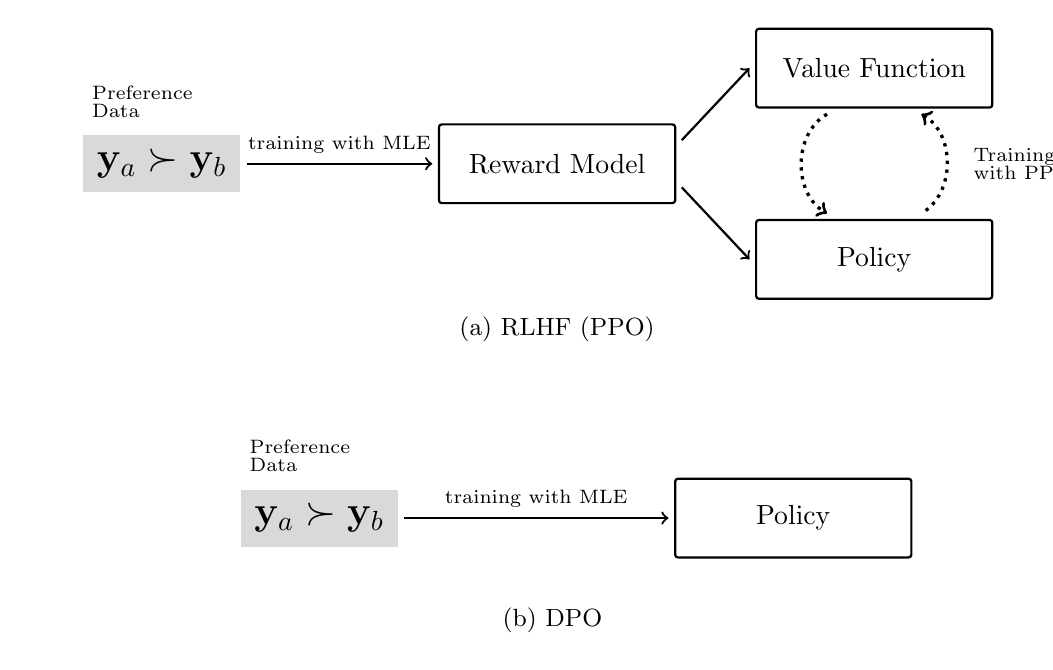
\begin{tikzpicture}
	
\def\ssep{0.9cm}

\tikzstyle{lnode} = [minimum width=3cm,minimum height=1.0cm,inner sep=2pt,draw,thick,fill=white,rounded corners=1pt];

%%% RLHF
\begin{scope}

\node [anchor=west,fill=gray!30,inner sep=5pt] (preferencedata) at (0,0) {\Large{$\mathbf{y}_a \succ \mathbf{y}_b$}};
\node [anchor=south west,align=left] (preferencelabel) at ([yshift=0.1cm]preferencedata.north west) {\scriptsize{Preference}\\[-0.2cm] \scriptsize{Data}};

\node [lnode,anchor=west] (rewardmodel) at ([xshift=2.5cm]preferencedata.east) {Reward Model};

\node [lnode,anchor=south west] (valuefunction) at ([xshift=1.0cm,yshift=0.7cm]rewardmodel.east) {Value Function};

\node [lnode,anchor=north west] (policy) at ([xshift=1.0cm,yshift=-0.7cm]rewardmodel.east) {Policy};

\draw [->,thick] ([xshift=2pt]preferencedata.east)--([xshift=-2pt]rewardmodel.west) node [pos=0.5,above,align=left] {\scriptsize{training with MLE}};

\draw [->,thick] ([xshift=2pt,yshift=0.3cm]rewardmodel.east) -- ([xshift=-2pt,yshift=0.0cm]valuefunction.west);
\draw [->,thick] ([xshift=2pt,yshift=-0.3cm]rewardmodel.east) -- ([xshift=-2pt,yshift=0.0cm]policy.west);

\draw [->,dotted,very thick] ([xshift=-0.6cm,yshift=-2pt]valuefunction.south) .. controls +(-150:0.5cm) and +(150:0.5cm) .. ([xshift=-0.6cm,yshift=2pt]policy.north);
\draw [<-,dotted,very thick] ([xshift=0.6cm,yshift=-2pt]valuefunction.south) .. controls +(-30:0.5cm) and +(30:0.5cm) .. ([xshift=0.6cm,yshift=2pt]policy.north) node [pos=0.5,right,xshift=0.2cm,align=left] {\scriptsize{Training}\\[-0.2cm] \scriptsize{with PPO}};

\node [anchor=north] (caption) at ([yshift=-1.3cm]rewardmodel.south) {\small{(a) RLHF (PPO)}};

\end{scope}

%%% DPO
\begin{scope}[yshift=-4.5cm]

\node [anchor=west,fill=gray!30,inner sep=5pt] (preferencedata) at (2cm,0) {\Large{$\mathbf{y}_a \succ \mathbf{y}_b$}};
\node [anchor=south west,align=left] (preferencelabel) at ([yshift=0.1cm]preferencedata.north west) {\scriptsize{Preference}\\[-0.2cm] \scriptsize{Data}};

\node [lnode,anchor=west] (policy) at ([xshift=3.5cm]preferencedata.east) {Policy};

\draw [->,thick] ([xshift=2pt]preferencedata.east)--([xshift=-2pt]policy.west) node [pos=0.5,above,align=left] {\scriptsize{training with MLE}};


\node [anchor=north west] (caption) at ([xshift=-2.3cm,yshift=-0.5cm]policy.south west) {\small{(b) DPO}};

\end{scope}

\end{tikzpicture}
\end{center}

\caption{Standard RLHF (PPO) vs. DPO. In RLHF, the human preference data is used to train a reward model, which is then employed in training the policy as well as the value function. In DPO, the use of human preference data is more direct, and the policy is trained on this data without the need for reward model training.}
\label{fig:rlhf-vs-dpo}
\end{figure}

Before deriving the DPO objective, let us first review the objective of policy training used in RLHF. As discussed in Section \ref{sec:rlhf-training-llms}, the policy is typically trained by optimizing a loss function with a penalty term. The DPO method assumes a simple loss function where the quality of the output $\mathbf{y}$ given the input $\mathbf{x}$ is evaluated by the reward model $r(\mathbf{x},\mathbf{y})$. The training objective is thus given by
\begin{eqnarray}
\tilde{\theta} & = & \argmin_{\theta} \mathbb{E}_{\mathbf{x} \sim \mathcal{D}} \mathbb{E}_{\mathbf{y} \sim \pi_{\theta}(\cdot|\mathbf{x})} \big[ \underbrace{-r(\mathbf{x},\mathbf{y})}_{\text{loss}} + \beta \underbrace{(\log \pi_{\theta}(\mathbf{y}|\mathbf{x}) - \log \pi_{\theta_{\mathrm{ref}}}(\mathbf{y}|\mathbf{x}) )}_{\text{penalty}} \big]. \label{eq:dpo-basic-objective}
\end{eqnarray}

\noindent Note that in this optimization problem, only the term $\pi_{\theta}(\mathbf{y}|\mathbf{x})$ depends on the target policy $\pi_{\theta}(\cdot)$. Both the reward model $r(\mathbf{x}, \mathbf{y})$ and the reference model $\pi_{\theta_{\mathrm{ref}}}(\mathbf{y}|\mathbf{x})$ are assumed to be fixed given $\mathbf{x}$ and $\mathbf{y}$. This is a strong assumption compared with PPO, but as will be shown later, it simplifies the problem and is important for deriving the DPO objective.

Since $\theta$ is the variable we want to optimize, we rearrange the right-hand side of Eq. (\ref{eq:dpo-basic-objective}) to make the dependence on $\theta$ explicit:
\begin{eqnarray}
&    & \tilde{\theta} \nonumber \\
& = & \argmin_{\theta} \mathbb{E}_{\mathbf{x} \sim \mathcal{D}} \mathbb{E}_{\mathbf{y} \sim \pi_{\theta}(\cdot|\mathbf{x})} \big[ \beta \log \pi_{\theta}(\mathbf{y}|\mathbf{x}) - \beta \log \pi_{\theta_{\mathrm{ref}}}(\mathbf{y}|\mathbf{x}) - r(\mathbf{x},\mathbf{y}) \big] \nonumber \\
& = & \argmin_{\theta} \mathbb{E}_{\mathbf{x} \sim \mathcal{D}} \mathbb{E}_{\mathbf{y} \sim \pi_{\theta}(\cdot|\mathbf{x})} \big[ \log \pi_{\theta}(\mathbf{y}|\mathbf{x}) - \big(\log \pi_{\theta_{\mathrm{ref}}}(\mathbf{y}|\mathbf{x}) + \frac{1}{\beta} r(\mathbf{x},\mathbf{y}) \big) \big] \nonumber \\
& = & \argmin_{\theta} \mathbb{E}_{\mathbf{x} \sim \mathcal{D}} \mathbb{E}_{\mathbf{y} \sim \pi_{\theta}(\cdot|\mathbf{x})} \Big[ \underbrace{\log \pi_{\theta}(\mathbf{y}|\mathbf{x})}_{\text{dependent on $\theta$}} - \underbrace{\log \Big(\pi_{\theta_{\mathrm{ref}}}(\mathbf{y}|\mathbf{x}) \exp \big(\frac{1}{\beta} r(\mathbf{x},\mathbf{y}) \big) \Big)}_{\text{not dependent on $\theta$}} \Big].
\label{eq:dpo-raw-objective-with-no-normalization}
\end{eqnarray}

This equation defines the objective function as the difference between the log-probability of the policy and another function of $\mathbf{y}$. This form of the objective function is not ideal, as we usually prefer to see the difference between two distributions, so that we can interpret this difference as some kind of divergence between the distributions. A simple idea is to convert the second term (i.e., $ \log \pi_{\theta_{\mathrm{ref}}}(\mathbf{y}|\mathbf{x}) \exp(\frac{1}{\beta} r(\mathbf{x},\mathbf{y}))$) into a log-probability distribution over the domain of $\mathbf{y}$. If we treat $ \pi_{\theta_{\mathrm{ref}}}(\mathbf{y}|\mathbf{x}) \exp(\frac{1}{\beta} r(\mathbf{x},\mathbf{y}))$ as an unnormalized probability of $y$, we can convert it into a normalized probability by dividing it by a normalization factor:
\begin{eqnarray}
Z(\mathbf{x}) & = & \sum_{\mathbf{y}} \pi_{\theta_{\mathrm{ref}}}(\mathbf{y}|\mathbf{x}) \exp \big(\frac{1}{\beta} r(\mathbf{x},\mathbf{y}) \big).
\end{eqnarray}

Hence we can define a probability distribution by
\begin{eqnarray}
\pi^*(\mathbf{y}|\mathbf{x}) & = & \frac{\pi_{\theta_{\mathrm{ref}}}(\mathbf{y}|\mathbf{x}) \exp \big(\frac{1}{\beta} r(\mathbf{x},\mathbf{y}) \big)}{Z(\mathbf{x})}.
\end{eqnarray}

We then rewrite Eq. (\ref{eq:dpo-raw-objective-with-no-normalization}) as
\begin{eqnarray}
\tilde{\theta} & = & \argmin_{\theta} \mathbb{E}_{\mathbf{x} \sim \mathcal{D}} \mathbb{E}_{\mathbf{y} \sim \pi_{\theta}(\cdot|\mathbf{x})} \Big[ \log \pi_{\theta}(\mathbf{y}|\mathbf{x}) - \log \frac{\pi_{\theta_{\mathrm{ref}}}(\mathbf{y}|\mathbf{x}) \exp \big(\frac{1}{\beta} r(\mathbf{x},\mathbf{y}) \big)}{Z(\mathbf{x})} \nonumber \\
& & \hspace{10.5em} - \log Z(\mathbf{x}) \Big] \nonumber \\
& = & \argmin_{\theta} \mathbb{E}_{\mathbf{x} \sim \mathcal{D}} \mathbb{E}_{\mathbf{y} \sim \pi_{\theta}(\cdot|\mathbf{x})} \Big[ \log \pi_{\theta}(\mathbf{y}|\mathbf{x}) - \log \pi^{*}(\mathbf{y}|\mathbf{x}) - \log Z(\mathbf{x}) \Big] \nonumber \\
& = & \argmin_{\theta} \mathbb{E}_{\mathbf{x} \sim \mathcal{D}} \bigg[ \mathbb{E}_{\mathbf{y} \sim \pi_{\theta}(\cdot|\mathbf{x})} \Big[ \log \pi_{\theta}(\mathbf{y}|\mathbf{x}) - \log \pi^{*}(\mathbf{y}|\mathbf{x}) \Big] \nonumber \\
&  & \hspace{6.5em} - \mathbb{E}_{\mathbf{y} \sim \pi_{\theta}(\cdot|\mathbf{x})} \big[ \log Z(\mathbf{x}) \big] \bigg] \nonumber \\
& = & \argmin_{\theta} \mathbb{E}_{\mathbf{x} \sim \mathcal{D}} \Big[ \underbrace{D_{\mathrm{KL}} \big(\pi_{\theta}(\cdot|\mathbf{x})\ \|\ \pi^{*}(\cdot|\mathbf{x}) \big)}_{\text{KL divergence}} - \underbrace{\log Z(\mathbf{x})}_{\text{constant wrt. $\theta$}} \Big].
\end{eqnarray}

Since $\log Z(\mathbf{x})$ is independent of $\theta$, it does not affect the result of the $\argmin_{\theta}$ operation, and can be removed from the objective. Now we obtain a new training objective which finds the optimal policy $\pi_{\theta}$ by minimizing the KL divergence between $\pi_{\theta}(\cdot|\mathbf{x})$ and $\pi^{*}(\cdot|\mathbf{x})$
\begin{eqnarray}
\tilde{\theta} & = & \argmin_{\theta} \mathbb{E}_{\mathbf{x} \sim \mathcal{D}} \Big[ D_{\mathrm{KL}} \big(\pi_{\theta}(\cdot|\mathbf{x})\ \|\ \pi^{*}(\cdot|\mathbf{x}) \big) \Big].
\end{eqnarray}

Clearly, the solution to this optimization problem is given by
\begin{eqnarray}
\pi_{\theta}(\mathbf{y}|\mathbf{x}) & = & \pi^{*}(\mathbf{y}|\mathbf{x}) \nonumber \\
& = & \frac{\pi_{\theta_{\mathrm{ref}}}(\mathbf{y}|\mathbf{x}) \exp \big(\frac{1}{\beta} r(\mathbf{x},\mathbf{y}))}{Z(\mathbf{x})}.
\end{eqnarray}

Given this equation, we can express the reward $r(\mathbf{x},\mathbf{y})$ using the target model $\pi_{\theta}(\mathbf{y}|\mathbf{x})$, the reference model $\pi_{\theta_{\mathrm{ref}}}(\mathbf{y}|\mathbf{x})$, and the normalization factor $Z(\mathbf{x})$:
\begin{eqnarray}
r(\mathbf{x},\mathbf{y}) & = & \beta \left(\log \frac{\pi_{\theta}(\mathbf{y}|\mathbf{x})}{\pi_{\theta_{\mathrm{ref}}}(\mathbf{y}|\mathbf{x})} + \log Z(\mathbf{x}) \right). \label{eq:dpo-reward-model-expression}
\end{eqnarray}

This is interesting because we initially seek to learn the policy $\pi_{\theta}(\cdot)$ using the reward model $r(\mathbf{x},\mathbf{y})$, but eventually obtain a representation of the reward model based on the policy. Given the reward model defined in Eq. (\ref{eq:dpo-reward-model-expression}), we can apply it to the Bradley-Terry model to calculate the preference probability (also see Section \ref{sec:training-reward-models}):
\begin{eqnarray}
\mathrm{Pr}_{\theta}(\mathbf{y}_a \succ \mathbf{y}_b | \mathbf{x}) & = & \mathrm{Sigmoid}(r(\mathbf{x},\mathbf{y}_a)-r(\mathbf{x},\mathbf{y}_b)) \nonumber \\
& = & \mathrm{Sigmoid}\bigg(\beta \Big(\log \frac{\pi_{\theta}(\mathbf{y}_a|\mathbf{x})}{\pi_{\theta_{\mathrm{ref}}}(\mathbf{y}_a|\mathbf{x})} + \log Z(\mathbf{x}) \Big) - \nonumber \\
&    & \hspace{4.3em} \beta \Big(\log \frac{\pi_{\theta}(\mathbf{y}_b|\mathbf{x})}{\pi_{\theta_{\mathrm{ref}}}(\mathbf{y}_b|\mathbf{x})} + \log Z(\mathbf{x}) \Big) \bigg) \nonumber \\
& = & \mathrm{Sigmoid}\bigg( \beta \log \frac{\pi_{\theta}(\mathbf{y}_a|\mathbf{x})}{\pi_{\theta_{\mathrm{ref}}}(\mathbf{y}_a|\mathbf{x})}  - \beta \log \frac{\pi_{\theta}(\mathbf{y}_b|\mathbf{x})}{\pi_{\theta_{\mathrm{ref}}}(\mathbf{y}_b|\mathbf{x})} \bigg).
\end{eqnarray}

This formula is elegant because it converts the difference in rewards into the difference in ratio functions, and we do not need to calculate the value of $Z(\mathbf{x})$. As a result, we no longer need a reward model, but only need the target policy and reference model to calculate the probability of preferences. Finally, we can train the target policy by minimizing the following DPO loss function
\begin{eqnarray}
\mathcal{L}_{\mathrm{dpo}}(\theta) & = & -\mathbb{E}_{(\mathbf{x},\mathbf{y}_a,\mathbf{y}_b) \sim \mathcal{D}_r} \big[ \log \mathrm{Pr}_{\theta}(\mathbf{y}_a \succ \mathbf{y}_b | \mathbf{x}) \big].
\end{eqnarray}

\noindent The form of this loss function is very similar to that used in training reward models in RLHF (see Eq. (\ref{eq:pairwise-reward-loss-expectation})). But it should be noted that the loss function here depends on the parameters of the policy (i.e., $\theta$) rather than the parameters of the reward model (i.e., $\phi$).

The main advantage of DPO lies in its simplicity and efficiency. The DPO objective is very straightforward --- it directly optimizes for preference-based feedback, rather than relying on separately developed reward models. Moreover, DPO is generally more sample-efficient, as it learns from a fixed dataset without the need for the computationally expensive sampling process used in PPO. This makes DPO a popular method for human preference alignment, especially when developing and applying reward models via reinforcement learning is challenging.

DPO can broadly be viewed as an \mindex{offline reinforcement learning} method, where the training data is pre-collected and fixed, and there is no exploration. In contrast, online reinforcement learning methods like PPO, which require exploring new states through interaction with the environment (using the reward model as a proxy), also have their unique advantages. One of the benefits of online reinforcement learning is that it allows the agent to continuously adapt to changes in the environment by learning from real-time feedback. This means that, unlike offline methods, online methods are not constrained by the static nature of pre-collected data and can discover new problem-solving strategies. In addition, exploration can help the agent cover a wider range of state-action pairs, thus improving generalization. This could be an important advantage for LLMs, as generalization is considered a critical aspect in applying such large models.

\subsection{Automatic Preference Data Generation}

\noindent Although learning from human preferences is an effective and popular method for aligning LLMs, annotating preference data is costly. Learning from human feedback not only suffers from limited scalability, but may also introduce bias because human feedback is inherently subjective. As a result, one can turn to AI feedback methods to address these scalability and consistency issues without the limitations associated with human annotators.

As with data generation for instruction fine-tuning, generating preference data using LLMs is straightforward. Given a set of inputs, we first use an LLM to generate pairs of outputs. Then, we prompt the LLM to determine the preferred output for each pair, given the corresponding input. Below is an example of prompting the LLM to generate a preference label for a pair of consumer service responses.

\vspace{0.5em}
\begin{tcolorbox}[frame empty]

\begingroup
\setlength{\leftskip}{2em}
\setlength{\rightskip}{2em}

Consider a customer service scenario where a customer poses a request. You will review two responses to this request. Please indicate which response is preferred. Note that a good response should be courteous, clear, and concise. It should address the customer's concern directly, provide helpful information or a solution, and maintain a positive tone.

\vspace{0.3cm}

Request:

\vspace{0.1cm}

\textit{Hello, I noticed that my order hasn't arrived yet, though it was scheduled to arrive several days ago. Could you please update me on its status? Thank you!}

\vspace{0.2cm}

Response A:

\vspace{0.1cm}

\textit{I'm very sorry for the delay and understand how disappointing this can be. We're doing our best to sort this out quickly for you.}

\vspace{0.3cm}

Response B:

\vspace{0.1cm}

\textit{Hey, stuff happens! Your package will get there when it gets there, no need to stress.}

\vspace{0.3cm}

\underline{Response A is preferred.}

\endgroup

\end{tcolorbox}
\vspace{0.5em}

Once we collect such preference labels, we can use them, along with the input and two responses, to train the reward model. We can, of course, consider providing a few demonstrations or using sophisticated prompting techniques, such as CoT, to improve labeling performance. For example, we can include in the prompt an example showing how and why one of the two responses is preferred based on a CoT rationale.

In addition to preference labels, we can also obtain the probability associated with each label \cite{lee-etal:2023rlaif}. A simple method is to extract the probabilities for the label tokens, such as ``A'' and ``B'', from the probabilities output by the LLM. We can then use the Softmax function or other normalization techniques to re-normalize these probabilities into a distribution over the labels. These probabilities of preferred labels can serve as pointwise supervision signals for training the reward model, as discussed in Section \ref{sec:better-reward-modeling}.

While scaling up AI data generation is easy, ensuring its accuracy and diversity remains crucial. Here, the data quality and diversity issues involve not only the labeling of preferences but also the inputs and outputs of the model. Therefore, we often need to use a variety of techniques to obtain large-scale, high-quality data. For example, one can generate diverse model outputs and annotations by using different LLMs, prompts, in-context demonstrations, and so on \cite{cui-etal:2024ultra}. \citet{dubois-etal:2024alpacafarm} report that the variability in pairwise preference data is important for training LLMs from either human or AI feedback.

While learning from AI feedback is highly scalable and generally more consistent than human feedback, this method is more suited to well-defined tasks where objective performance metrics are available. By contrast, learning from human feedback is more advantageous when aligning AI systems with human values, preferences, and complex real-world tasks that require understanding of subtle or subjective context. These methods can be combined to train LLMs that benefit from both human insights and the scalability of AI feedback.

\subsection{Step-by-step Alignment}

\noindent So far, our discussion of alignment has primarily focused on the use of reward models for evaluating entire input-output sequence pairs. These methods can be easily adapted to scenarios where the correctness of the output can be verified based on the final answer. For example, in the task of calculating a mathematical expression, a reward model can provide positive feedback if the answer is correct, and negative feedback if the answer is wrong. However, in many problems that require complex reasoning, simply examining the correctness of the final result is insufficient for learning. Imagine a student who is only given the final answer to a challenging math problem. Knowing whether the final answer is right or wrong does not help the student figure out where they went wrong and how to calculate the correct answer. A better approach would be to guide the student with a step-by-step breakdown of the problem-solving process and help the student understand the underlying concepts and logic behind these steps.

In Chapter \ChapterLLMPrompting, we studied CoT methods to prompt LLMs to explicitly write out intermediate steps or the reasoning process needed to reach a conclusion or solve a problem. We saw that breaking down a problem into smaller parts could make it easier to understand the solution path and increase the accuracy of the output. These methods can be naturally extended to the alignment of LLMs, that is, we supervise the model during the intermediate steps of reasoning. Consider a reasoning task where an LLM produces a sequence of reasoning steps $\mathbf{y} = \{\bar{\mathbf{y}}_1,...,\bar{\mathbf{y}}_{n_s}\}$ for the given input. The result of the reasoning is assumed to be contained in the last step $\bar{\mathbf{y}}_{n_s}$, and can be easily verified. For this reasoning problem, \citet{uesato-etal:2022solving} categorize LLM fine-tuning approaches into two classes:

\begin{itemize}
\item \vspace{0.5em} \mindex{Outcome-based Approaches}. Supervision occurs only when the end result is verified. This is a standard method for learning from human feedback we have discussed in this chapter. For example, the LLM is optimized to maximize some form of the reward $r(\mathbf{x},\mathbf{y})$.
\item \vspace{0.3em} \mindex{Process-based Approaches}. Supervision is applied to all intermediate steps in addition to the last step. To do this, we need to develop a reward model to give a supervision signal at each step, and design loss functions that can make use of such supervision signals.
\end{itemize}
\vspace{0.5em}

Figure \ref{fig:outcome-vs-process-based-approaches} shows two LLM outputs for an example math problem. Although the LLM gives the correct final answer in both cases, it makes mistakes during the problem-solving process in the second output. Outcome-based approaches overlook these mistakes and give positive feedback for the entire solution. By contrast, process-based approaches can take these mistakes into account and provide additional guidance on the detailed reasoning steps.

\begin{figure}[!t]
\centering
% !Mode:: "TeX:UTF-8"
% !TEX encoding = UTF-8 Unicode

\begin{center}
\begin{tikzpicture}
	
\def\ssep{0.9cm}

\tikzstyle{lnode} = [minimum width=3cm,minimum height=1.0cm,inner sep=2pt,draw,thick,fill=white,rounded corners=1pt];

%%% a math problem and corresponding reasoning paths
\begin{scope}


\node [anchor=west,align=left,minimum width=13.5cm,draw,thick,inner sep=6pt] (question) at (0,0) {\small{\textbf{Question} (from The International Junior Math Olympiad):}\\ \small{Jessica has a lot of apps on her phone. The number of apps she has is divisible by 5. If she}\\ \small{downloaded 10 more apps, she would still have less than 50 apps. What is the maximum \hspace{1cm}}\\ \small{original number of apps Jessica could have?}};

%%% response 1
\begin{scope}
\node [anchor=north west,align=left] (response1) at ([xshift=0.4cm,yshift=-0.3cm]question.south west) {\small{\textbf{Response 1}:}};

\node [anchor=north west,align=left] (y1) at ([xshift=0.1cm,yshift=-0.2cm]response1.south west) {\small{$x$ must be a multiple of $5$, i.e., }\\ \small{$x \equiv 0\ (\mathrm{mod}\ 5)$.}};
\node [anchor=west] (y1r) at ([xshift=5.5cm]y1.west) {{\color{gray!20} x}};
\node [anchor=north east] (y1label) at ([xshift=0.10cm,yshift=-0.00cm]y1.north west) {\footnotesize{$\bar{\mathbf{y}}_1$:}};

\node [anchor=north west,align=left] (y2) at ([yshift=-0.2cm]y1.south west) {\small{After downloading $10$ apps, the total}\\ \small{total number of apps should still be less}\\ \small{than $50$: $x + 10 < 50$. Solving this}\\ \small{inequality: $x < 40$.}};
\node [anchor=west] (y2r) at ([xshift=5.5cm]y2.west) {{\color{gray!20} x}};
\node [anchor=north east] (y2label) at ([xshift=0.15cm,yshift=-0.00cm]y2.north west) {\footnotesize{$\bar{\mathbf{y}}_2$:}};

\node [anchor=north west,align=left] (y3) at ([yshift=-0.2cm]y2.south west) {\small{Since $x$ must be a multiple of $5$ and }\\ \small{less than $40$, the largest value of $x$ is $35$.}};
\node [anchor=west] (y3r) at ([xshift=5.5cm]y3.west) {{\color{gray!20} x}};
\node [anchor=north east] (y3label) at ([xshift=0.10cm,yshift=-0.00cm]y3.north west) {\footnotesize{$\bar{\mathbf{y}}_3$:}};

\node [anchor=north west,align=left] (y4) at ([yshift=-0.2cm]y3.south west) {\small{Verify the result. If $x=35$, then after}\\ \small{downloading 10 apps, Jessica would}\\ \small{have: $35+10=45$ which satisfy}\\ \small{$45<50$.}};
\node [anchor=west] (y4r) at ([xshift=5.5cm]y4.west) {{\color{gray!20} x}};
\node [anchor=north east] (y4label) at ([xshift=0.10cm,yshift=-0.00cm]y4.north west) {\footnotesize{$\bar{\mathbf{y}}_4$:}};

\node [anchor=north west,align=left] (y5) at ([yshift=-0.2cm]y4.south west) {\small{The maximum original number of}\\ \small{apps is \underline{$35$}.}};
\node [anchor=west] (y5r) at ([xshift=5.5cm]y5.west) {{\color{gray!20} x}};
\node [anchor=north east] (y5label) at ([xshift=0.10cm,yshift=-0.00cm]y5.north west) {\footnotesize{$\bar{\mathbf{y}}_5$:}};

\begin{pgfonlayer}{background}
\node [inner sep=0pt,fill=gray!20]  [fit = (y1) (y1r)] (y1box) {};
\node [inner sep=0pt,fill=gray!20]  [fit = (y2) (y2r)] (y2box) {};
\node [inner sep=0pt,fill=gray!20]  [fit = (y3) (y3r)] (y3box) {};
\node [inner sep=0pt,fill=gray!20]  [fit = (y4) (y4r)] (y4box) {};
\node [inner sep=0pt,fill=gray!20]  [fit = (y5) (y5r)] (y5box) {};
\end{pgfonlayer}

\draw [->] ([xshift=-1.18cm,yshift=-0.3cm]y5.south) -- ([xshift=-1.18cm,yshift=0.1cm]y5.south);
\node [anchor=north] (answerlabel) at ([xshift=-1.18cm,yshift=-0.3cm]y5.south) {\footnotesize{correct}};

\end{scope}

%%% response 2
\begin{scope}
\node [anchor=west,align=left] (response2) at ([xshift=5cm]response1.east) {\small{\textbf{Response 2}:}};

\node [anchor=north west,align=left] (y1) at ([xshift=0.1cm,yshift=-0.2cm]response2.south west) {\small{The number of apps is divisible by $5$,}\\ \small{so $x$ must be a multiple of $5$.}};
\node [anchor=west] (y1r) at ([xshift=5.5cm]y1.west) {{\color{gray!20} x}};
\node [anchor=north east] (y1label) at ([xshift=0.10cm,yshift=-0.00cm]y1.north west) {\footnotesize{$\bar{\mathbf{y}}_1$:}};

\node [anchor=north west,align=left] (y2) at ([yshift=-0.2cm]y1.south west) {\small{If she downloads 10 more apps, her}\\ \small{new total will be $x+10$, and  this must}\\ \small{be less than 50. Therefore, $x + 10 < 50$.}\\ \small{Simplifying this gives $x < 40$.}};
\node [anchor=west] (y2r) at ([xshift=5.5cm]y2.west) {{\color{gray!20} x}};
\node [anchor=north east] (y2label) at ([xshift=0.15cm,yshift=-0.00cm]y2.north west) {\footnotesize{$\bar{\mathbf{y}}_2$:}};

\node [anchor=north west,align=left] (y3) at ([yshift=-0.2cm]y2.south west) {\small{$x$ must be less than or equal to}\\ \small{the largest multiple of $5$, which is $40$.}};
\node [anchor=west] (y3r) at ([xshift=5.5cm]y3.west) {{\color{red!20} x}};
\node [anchor=north east] (y3label) at ([xshift=0.10cm,yshift=-0.00cm]y3.north west) {\footnotesize{$\bar{\mathbf{y}}_3$:}};

\node [anchor=north west,align=left] (y4) at ([yshift=-0.2cm]y3.south west) {\small{But $x + 10$ should not be more}\\ \small{than or equal to 50. So we need to}\\ \small{subtract $5$ from $40$.}};
\node [anchor=west] (y4r) at ([xshift=5.5cm]y4.west) {{\color{red!20} x}};
\node [anchor=north east] (y4label) at ([xshift=0.10cm,yshift=-0.00cm]y4.north west) {\footnotesize{$\bar{\mathbf{y}}_4$:}};

\node [anchor=north west,align=left] (y5) at ([yshift=-0.2cm]y4.south west) {\small{Therefore, the final result is \underline{$35$}.}};
\node [anchor=west] (y5r) at ([xshift=5.5cm]y5.west) {{\color{gray!20} x}};
\node [anchor=north east] (y5label) at ([xshift=0.10cm,yshift=-0.00cm]y5.north west) {\footnotesize{$\bar{\mathbf{y}}_5$:}};

\begin{pgfonlayer}{background}
\node [inner sep=0pt,fill=gray!20]  [fit = (y1) (y1r)] (y1box) {};
\node [inner sep=0pt,fill=gray!20]  [fit = (y2) (y2r)] (y2box) {};
\node [inner sep=0pt,fill=red!20]  [fit = (y3) (y3r)] (y3box) {};
\node [inner sep=0pt,fill=red!20]  [fit = (y4) (y4r)] (y4box) {};
\node [inner sep=0pt,fill=gray!20]  [fit = (y5) (y5r)] (y5box) {};
\end{pgfonlayer}

\draw [->] ([xshift=1.95cm,yshift=-0.3cm]y5.south) -- ([xshift=1.95cm,yshift=0.1cm]y5.south);
\node [anchor=north] (answerlabel) at ([xshift=1.95cm,yshift=-0.3cm]y5.south) {\footnotesize{correct}};

\node [anchor=north east,fill=white,draw,rounded corners=1pt,inner sep=3pt] (y3wrong) at ([xshift=0.05cm,yshift=0.05cm]y3box.north east) {\tiny{problematic}};
\node [anchor=north east,fill=white,draw,rounded corners=1pt,inner sep=3pt] (y4wrong) at ([xshift=0.05cm,yshift=0.05cm]y4box.north east) {\tiny{problematic}};


\end{scope}

\end{scope}

\end{tikzpicture}
\end{center}

\caption{Two LLM responses to a math problem. In response 1, both the final result and all the reasoning steps are correct. In response 2, the final result is correct, but there are mistakes in the reasoning process (highlighted in red). For outcome-based approaches, both responses are considered correct. For process-based approaches, the mistakes in response 2 can be considered in reward modeling.}
\label{fig:outcome-vs-process-based-approaches}
\end{figure}

A key challenge for process-based approaches is that we need to get step-level feedback during a (potentially) long reasoning path. We can collect or generate reasoning paths corresponding to problems from existing datasets. Human experts then annotate each step with correctness labels. These annotations can be used to directly train LLMs or as rewards in reward modeling. However, in practice, richer annotations are often employed \cite{lightman-etal:2024lets}. In addition to the \textit{correct} and \textit{incorrect} labels, a step can also be labeled as \textit{neutral} to indicate that while the step may be technically correct, it might still be problematic within the overall reasoning process. Furthermore, to improve the efficiency of data annotation, techniques such as active learning can be employed. Identifying obvious errors usually does not significantly contribute to learning from reasoning mistakes. Instead, annotating steps that the model confidently considers correct but are actually problematic is often more effective.

Given a set of step-level annotated reasoning paths and corresponding inputs, we can train a reward model to provide feedback for supervising policy learning. The reward model can be treated as a classification model, and so its architecture can be a Transformer decoder with a Softmax layer stacked on top. At step $k$, the reward model takes both the problem description (denoted by $\mathbf{x}$) and the reasoning steps generated so far (denoted by $\bar{\mathbf{y}}_{\le k}$) as input and outputs a probability distribution over the label set $\{\text{\textit{correct}}, \text{\textit{incorrect}}\}$ or $\{\text{\textit{correct}}, \text{\textit{incorrect}}, \text{\textit{neutral}}\}$. Then the learned reward model is used to evaluate reasoning paths by assessing the correctness of each step. A simple method to model correctness is to count the number of steps that are classified as \textit{correct}, given by
\begin{eqnarray}
r(\mathbf{x},\mathbf{y}) & = & \sum_{k=1}^{n_s} \delta(\text{\textit{correct}},C(\mathbf{x},\bar{\mathbf{y}}_{\le k})),
\end{eqnarray}

\noindent where $C(\mathbf{x},\bar{\mathbf{y}}_{\le k})$ denotes the label with the maximum probability. We can also use log-probabilities of classification to define the reward of the entire path
\begin{eqnarray}
r(\mathbf{x},\mathbf{y}) & = &  \sum_{k=1}^{n_s} \log \Pr(\textit{correct}|\mathbf{x},\bar{\mathbf{y}}_{\le k}),
\end{eqnarray}

\noindent where $\Pr(\textit{correct}|\mathbf{x},\bar{\mathbf{y}}_{\le k})$ denotes the probability of the \textit{correct} label generated by the reward model. The reward score $r(\mathbf{x},\mathbf{y})$ can then be used to train the policy in RLHF as usual.

While we restrict our discussion to math problems, the approaches described here are general and can be applied to a wide variety of tasks that involve multi-step reasoning and decision-making. Moreover, we can consider various aspects when assessing the quality of a step, rather than just its correctness. For example, in dialogue systems, responses must not only be accurate but also contextually appropriate across multiple turns of conversation. If a model provides a correct response but fails to maintain coherence in the context of the ongoing dialogue, step-level feedback could help the model identify and correct such discrepancies. Also note that the process-based approaches are related to the fine-grained reward modeling approaches discussed in Section \ref{sec:fine-grained-rewards}. All these approaches essentially aim to provide more detailed supervision to LLMs by breaking their outputs into smaller, more manageable steps. However, process-based feedback focuses more on evaluating the correctness of a step based on its preceding steps, while the approaches in Section \ref{sec:fine-grained-rewards} emphasize evaluating each step independently.

The idea of aligning LLMs step by step has great application potential, especially considering the recent shift towards more complex reasoning tasks in the use of LLMs. For example, both the GPT o1 and o3 models are designed with more advanced reasoning techniques (such as long internal CoT) to solve challenging problems like scientific and mathematical reasoning \cite{openai:2024learning}. These tasks often rely on long and complex reasoning paths, and therefore, it seems essential to introduce detailed supervision signals in the reasoning process. Moreover, from a practical perspective, effective supervision on long reasoning paths not only improves reasoning performance, but also helps the model eliminate unnecessary reasoning steps, thereby reducing reasoning complexity and improving efficiency.

\subsection{Inference-time Alignment}

\noindent So far in this section, we have explored a variety of methods to align models with human preferences and annotations. However, one of the significant limitations of many such methods is that LLMs must be fine-tuned. For RLHF and its variants, training LLMs with reward models can be computationally expensive and unstable, leading to increased complexity and costs when applying these approaches. In this case, we can consider performing alignment at inference time, thus avoiding the additional complexity and effort involved.

One simple way to achieve inference-time alignment is to use the reward model to select the best one from $N$ alternative outputs generated by the LLM, a method known as \mindex{Best-of-$N$ sampling} (\mindex{BoN sampling}). We can consider BoN sampling as a form of reranking. In fact, reranking methods have been widely used in NLP tasks, such as machine translation, for a long time. They are typically applied in situations where training complex models is costly. In such cases, directly reranking the outputs allows for the incorporation of these complex models at a very low cost\footnote{Reranking methods can also help us explore what are known as model errors and search errors, although these issues are not often discussed in the context of LLMs. For example, suppose we have an old model and a new, more powerful model. We can use the new model to select the best output from the $N$-best list of the old model as the oracle output. The performance difference between the oracle output and the top-1 output of the original $N$-best list reflects the performance gain brought by the new model. If the performance gain is significant, we can say that the old model has more model errors. If the gain is small, it may indicate that the issue lies in search errors, as the best candidates were not found.}.

In the BoN sampling process, the LLM takes the input sequence $\mathbf{x}$ and generates $N$ different output sequences $\{\hat{\mathbf{y}}_1,...,\hat{\mathbf{y}}_N\}$:
\begin{eqnarray}
\{\hat{\mathbf{y}}_1,...,\hat{\mathbf{y}}_N\} & = & \mathop{\mathrm{argTopN}}_{\mathbf{y}} \left[ \Pr(\mathbf{y}|\mathbf{x}) \right],
\end{eqnarray}

\noindent where the $\mathrm{argTopN}$ operation returns the top-$N$ outputs that maximize the function $\Pr(\mathbf{y}|\mathbf{x})$. These outputs can be generated in a variety of ways, depending on the search algorithm used by the model (e.g., sampling or beam search). Once the $N$-best output candidates are generated, the reward model is used to evaluate and select the best one:
\begin{eqnarray}
\hat{\mathbf{y}}_{\mathrm{best}} & = & \argmax_{\hat{\mathbf{y}} \in \{\hat{\mathbf{y}}_1,\ldots,\hat{\mathbf{y}}_N\}} r(\mathbf{x},\hat{\mathbf{y}}).
\end{eqnarray}

It is worth noting that the result of BoN sampling is also influenced by the diversity of the $N$-best list. This is a common issue with most reranking methods. Ideally, the $N$-best output candidates should have relatively high quality but be sufficiently different from each other. In many text generation systems, the $N$-best outputs are very similar, often differing by just one or two words. The diversity issue is even more challenging in LLMs, as the $N$-best outputs generated by an LLM can differ in wording, yet their semantic meanings are often quite similar. In practice, one can adjust the model hyperparameters and/or use different LLMs to generate more diverse output candidates for reranking. Nevertheless, as with many practical systems, we need to make a trade-off between selecting high-quality candidates and ensuring sufficient variation in the generated outputs.

BoN sampling can be used for training LLMs as well. A closely related method is \mindex{rejection sampling}. In this method, we first select the ``best'' outputs from the $N$-best lists using the reward model, and then take these selected outputs to fine-tune the LLM. In this way, we can introduce human preferences into the training of LLMs using a much simpler approach compared to RLHF. Many LLMs have adopted rejection sampling for fine-tuning \cite{nakano-etal:2021webgpt,touvron-etal:2023llama2}.

%----------------------------------------------------------------------------------------
% NEW SECTION
%----------------------------------------------------------------------------------------

\section{Summary}

In this chapter, we have explored a range of techniques for aligning LLMs. In particular, we have discussed fine-tuning methods that enable LLMs to follow instructions and align them with human preferences. One of the benefits of fine-tuning LLMs is computational efficiency. Unlike pre-training based on large-scale neural network optimization, fine-tuning is a post-training step and so is less computationally expensive. Moreover, it is better suited to address problems that are not easily solved in pre-training, such as human value alignment. The widespread attention to AI alignment has also led to a surge of research papers on this topic, which makes it difficult to comprehensively cover all recent techniques. However, we have tried to provide a relatively detailed introduction to the fundamental approaches to alignment, such as instruction fine-tuning and RLHF.

While we have focused on LLM alignment techniques in this chapter, the term \textit{AI alignment} is a wide-ranging concept. It generally refers to the process of ensuring that the behavior of an AI system aligns with human values, goals, and expectations. The idea of AI alignment can be traced back to the early days of AI. A widely cited description of AI alignment comes from an article by the mathematician and computer scientist Norbert Wiener \cite{wiener:1960some}. The quote is as follows

\vspace{0.5em}
\begin{center}
\parbox{0.8\linewidth}{
\textit{If we use, to achieve our purposes, a mechanical agency with whose operation we cannot efficiently interfere ... we had better be quite sure that the purpose put into the machine is the purpose which we really desire.}
}
\end{center}
\vspace{0.5em}

At that time, alignment was not yet a central concern in AI research. But today, it greatly influences the design of various AI systems. For example, in robotics, alignment is critical to ensuring that autonomous robots safely interact with humans and their environments. In autonomous driving, cars must not only follow traffic laws but also make complex, real-time decisions that prioritize human safety, avoid accidents, and navigate ethical dilemmas.

In current AI research, alignment is often approached by developing a surrogate objective that is analogous to the true goal and steering the AI system towards this objective. However, designing the objective of AI alignment is very difficult. One reason is that human values are diverse and often context-dependent, making it difficult to distill them into a single, universally applicable objective function. Also, the complexity of real-world environments, where values and goals often conflict or evolve over time, further complicates alignment efforts. Even if we could define an appropriate objective, AI systems may find unintended ways to achieve it, leading to ``misaligned'' outcomes that still technically satisfy the objective but in a harmful or counterproductive way.

These challenges continue to motivate AI research towards more aligned systems, either through developing new mechanisms for perceiving the world or more efficient and generalizable methods to adapt these systems to given tasks. More importantly, as AI systems become more powerful and intelligent, especially given that recent advances in LLMs have shown remarkable capabilities in dealing with many challenging problems, the need for AI alignment has become more urgent. Researchers have started to be concerned with AI safety and warn the community that they need to develop and release AI systems with great caution to prevent these systems from being misaligned \cite{russell:2019human,bengio-etal:2024managing}.

